\documentclass[journal]{IEEEtran}
% 共享文档信息 (可以从主文档和补充文档中调用)

% 只保留一次，放在文件最前面
\usepackage{amsmath,amssymb,amsfonts}
\usepackage{algorithm,algorithmic}
\usepackage{array}
\usepackage{graphicx}
\usepackage{xcolor}
\usepackage{url}
% \usepackage{hyperref}
\usepackage[pdfencoding=auto, psdextra]{hyperref}
\usepackage[all]{hypcap}
\usepackage{cleveref}
\usepackage{lipsum}
\usepackage{booktabs, multirow, setspace}
\usepackage{tikz}
\usetikzlibrary{arrows.meta, positioning, fit, shapes.misc}
\usepackage{enumitem}
\usepackage{subcaption}
\usepackage{nicefrac, xspace, mathrsfs, bm}
\usepackage{cite}
\usepackage{nameref}
\usepackage{stfloats}
\usepackage{textcomp}
\usepackage[utf8]{inputenc}
\usepackage[T1]{fontenc}
\hyphenation{op-tical net-works semi-conduc-tor IEEE-Xplore}
\usepackage{microtype}
% \usepackage{caption}
\captionsetup[table]{
  labelfont=sc,        % 标签使用small caps
  textfont=sc,         % 文本使用small caps
  labelsep=newline,    % 标签和标题之间换行
  justification=centering  % 居中对齐
}
\usepackage{newtxtext,newtxmath}  % Times字体包
%-----------------------------数学符号新命令------------------------------
\newcommand{\eucalB}{\EuScript{B}}
\newcommand{\eucalP}{\EuScript{P}}
\newcommand{\Var}{\mathrm{Var}}
\newcommand{\Cov}{\mathrm{Cov}}
\newcommand{\Ex}{\mathsf{E}}
\newcommand{\Prob}{\mathsf{P}}
\newcommand{\one}{\mathbbm{1}}
\newcommand{\One}{\bm{1}}
\newcommand{\zero}{\bm{0}}
\newcommand{\RR}{\mathbb{R}}
\newcommand{\ZZ}{\mathbb{Z}}
\newcommand{\EE}{\mathbb{E}}
\newcommand{\PP}{\mathbb{P}}
\newcommand{\Rp}{\RR_+}
\newcommand{\TT}{\mathbb{T}}
\newcommand{\NN}{\mathbb{N}}
\newcommand{\VV}{\mathbb{V}}
\newcommand{\diff}{\mathrm{d}}
\newcommand{\prox}{\mathrm{prox}}
\newcommand{\rprox}{\mathrm{rprox}}
\newcommand{\ran}{\mathrm{ran}}
\newcommand{\Id}{\mathrm{Id}}
\newcommand{\e}{\mathrm{e}}
\newcommand{\bA}{\bm{A}}
\newcommand{\bB}{\bm{B}}
\newcommand{\bH}{\bm{H}}
\newcommand{\bF}{\bm{F}}
\newcommand{\bS}{\bm{S}}
\newcommand{\bX}{\bm{X}}
\newcommand{\bx}{\bm{x}}
\newcommand{\bb}{\bm{b}}
\newcommand{\bc}{\bm{c}}
\newcommand{\br}{\bm{r}}
\newcommand{\bbeta}{\bm{\beta}}
\newcommand{\bt}{\bm{t}}
% \newcommand{\eproof}{\hfill $\square$}
\newcommand{\bh}{\bm{h}}
\newcommand{\bu}{\bm{u}}
\newcommand{\bz}{\bm{z}}
\newcommand{\ba}{\bm{a}}
\newcommand{\by}{\bm{y}}
\newcommand{\be}{\bm{e}}
\newcommand{\bU}{\bm{U}}
\newcommand{\bZ}{\bm{Z}}
\newcommand{\bY}{\bm{Y}}
\newcommand{\blmbd}{\bm{\lambda}}
\newcommand{\bLmbd}{\bm{\Lambda}}
\newcommand{\bg}{\bm{g}}
\newcommand{\bd}{\bm{d}}
\DeclareMathOperator*{\argmin}{\mathrm{argmin}}
\DeclareMathOperator*{\Argmin}{\mathrm{Argmin}}
\DeclareMathOperator*{\minimize}{\mathrm{minimize}\,}
\DeclareMathOperator*{\maximize}{\mathrm{maximize}}
\DeclareMathOperator*{\argmax}{\mathrm{argmax}}
\DeclareMathOperator*{\Diag}{\mathrm{Diag}}
\newcommand{\calX}{\mathcal{X}}
\newcommand{\calY}{\mathcal{Y}}
\newcommand{\calB}{\mathcal{B}}
\newcommand{\calL}{\mathcal{L}}
\newcommand{\calG}{\mathcal{G}}
\newcommand{\calS}{\mathcal{S}}
\newcommand{\calC}{\mathcal{C}}
\newcommand{\calJ}{\mathcal{J}}
\newcommand{\calD}{\mathcal{D}}
\newcommand{\calQ}{\mathcal{Q}}
\newcommand{\calO}{\mathcal{O}}
\newcommand{\ent}{\mathrm{ent}}
% \newcommand{\diag}{\mathrm{diag}}
\newcommand{\dom}{\mathrm{dom}}
\newcommand{\interior}{\mathrm{int}}
\newcommand{\zer}{\mathrm{zer}}
\newcommand{\epi}{\mathrm{epi}}
\newcommand{\amax}{a_{\max}}
\newcommand{\amin}{a_{\min}}
\newcommand{\bmax}{b_{\max}}
\newcommand{\bmin}{b_{\min}}
\newcommand{\bp}{\bm{p}}
\newcommand{\bmu}{\bm{\mu}}
\newcommand{\bD}{\bm{D}}
\newcommand{\mW}{\mathrm{W}}
\newcommand{\bv}{\bm{v}}
\newcommand{\bw}{\bm{w}}
\newcommand{\ta}{\tilde{a}}
\newcommand{\tb}{\tilde{b}}
\newcommand{\tp}{\widetilde{\bp}}
\newcommand{\sumn}{\sum_{i=1}^n}
\newcommand{\sumQ}{\sum_{q=1}^Q}
\newcommand{\sumq}{\sum_{k=1}^q}
\newcommand{\summ}{\sum_{i=1}^m}
\newcommand{\sumd}{\sum_{i=1}^d}
\newcommand{\sumT}{\sum\limits_{ k =1}^{T}}
\newcommand{\sumTa}{\frac{1}{T} \sum\limits_{ k =1}^{T}}
\newcommand{\bC}{\bm{C}}
\newcommand{\bI}{\bm{I}}
\newcommand{\bM}{\bm{M}}
\newcommand{\bR}{\bm{R}}
\newcommand{\bV}{\bm{V}}
\newcommand{\bW}{\bm{W}}
\newcommand{\bxi}{\bm{\xi}}
\newcommand{\tmu}{\widetilde{\bmu}}
\newcommand{\tU}{\widetilde{\bU}}
\newcommand{\tV}{\widetilde{\bV}}
\newcommand{\tM}{\widetilde{\bM}}
\newcommand{\bDelta}{\bm{\Delta}}
\newcommand{\bs}{\bm{s}}
\newcommand{\ox}{\overline{x}}
\newcommand{\ob}{\overline{b}}
\newcommand{\op}{\overline{p}}
\newcommand{\obp}{\overline{\bp}}
\newcommand{\obmu}{\overline{\bmu}}
\newcommand{\obC}{\overline{\bC}}
\newcommand{\obD}{\overline{\bD}}
\newcommand{\bsigma}{\bm{\sigma}}
\newcommand{\bomega}{\bm{\omega}}
\newcommand{\tomega}{\widetilde{\omega}}
\newcommand{\tr}{\mathrm{tr}}
\newcommand{\an}{\mathrm{an}}
\newcommand{\bj}{\bm{j}}
\newcommand{\bG}{\bm{G}}
\newcommand{\bcalG}{\bm{\calG}}
\newcommand{\bcalK}{\bm{\calK}}
\newcommand{\bcalX}{\bm{\calX}}
\newcommand{\fX}{\mathfrak{X}}
\newcommand{\bfX}{\bm{\fX}}
\newcommand{\bell}{\bm{\ell}}
\newcommand{\bL}{\bm{L}}
\newcommand{\hy}{\widehat{y}}
\newcommand{\ul}[1]{\underline{#1}}
\newtheorem{assumption}{Assumption}
\newtheorem{definition}{Definition}
\newtheorem{lemma}{Lemma}
\newtheorem{theorem}{Theorem}
\renewcommand{\vec}{\mathrm{vec}}
\newtheorem{proof}{Proof}
\newenvironment{noproof}{\par\noindent\textbf{Proof.}\space}{\hfill\par}
\newtheorem{corollary}[theorem]{Corollary} 
\newtheorem{remark}{Remark}[section]  % 按节编号的注释环境
\newtheorem{proposition}{Proposition}
% \newtheorem{remark}[theorem]{Remark}  % 与theorem共享编号

\newcommand{\bcL}{\overline{\calL}}
\newcommand{\KL}{K\L\xspace}
\newcommand{\res}{\mathrm{res}}
\newcommand{\eproof}{\hfill $\square$}

\newcommand{\commyy}[1]{{\color{red}(yy: #1)}} % Yuan Yao's comments

\numberwithin{equation}{section}
\newcommand{\blue}[1]{\begin{color}{blue}#1\end{color}} 
\newcommand{\red}[1]{\begin{color}{red}#1\end{color}}

%% Packages and macros go here
\usepackage{lipsum}
\usepackage{amsfonts}
\usepackage{graphicx}
\usepackage{epstopdf}
\usepackage{algorithmic}
\ifpdf
  \DeclareGraphicsExtensions{.eps,.pdf,.png,.jpg}
\else
  \DeclareGraphicsExtensions{.eps}
\fi

% Prevent itemized lists from running into the left margin inside theorems and proofs
\usepackage{enumitem}
\setlist[enumerate]{leftmargin=.5in}
\setlist[itemize]{leftmargin=.5in}

% Add a serial/Oxford comma by default.
\newcommand{\creflastconjunction}{, and~}

\allowdisplaybreaks[2] 
% 允许更多浮动体
\setcounter{topnumber}{3}        % 页面顶部最多3个浮动体
\setcounter{bottomnumber}{2}     % 页面底部最多2个
\setcounter{totalnumber}{4}      % 每页最多4个浮动体
\setcounter{dbltopnumber}{4}     % 双栏页面顶部最多3个

\begin{document}

\title{DualHash: A Stochastic Primal-Dual Algorithm with Theoretical Guarantee for Deep Hashing}

% 作者信息
\author{Luxuan Li,
% ~\IEEEmembership{Student Member,~IEEE,}
      Xiao Wang, and  Chunfeng Cui$^{\ast}$
      %,~\IEEEmembership{Member,~IEEE,} 
% <-this % stops a space
\thanks{L. Li and C. Cui are with the School of Mathematical Sciences, Beihang University, Beijing 100191, China (e-mail: luxuanli@buaa.edu.cn; chunfengcui@buaa.edu.cn).}

\thanks{X. Wang is with the School of Computer Science and Engineering, Sun Yat-Sen University, Guangzhou 510006, China (e-mail: wxucas@outlook.com).}%
\thanks{$^{\ast}$Corresponding author.}}

% 页眉信息
\markboth{}
% ~Vol.~XX, No.~X, Month~YEAR}%
{Li \textit{et al.}: DualHash: A Stochastic Primal-Dual Algorithm for Deep Hashing}


\maketitle
\begin{abstract}
Deep hashing converts high-dimensional feature vectors into compact binary codes, enabling efficient large-scale retrieval. A fundamental challenge in deep hashing stems from the discrete nature of quantization in generating the codes. W-type regularizations, such as $||z|-1|$, have been proven effective as they encourage variables toward binary values. However, existing methods often directly optimize these regularizations without convergence guarantees. While proximal gradient methods offer a promising solution, the coupling between W-type regularizers and neural network outputs results in composite forms that generally lack closed-form proximal solutions. In this paper, we present a stochastic primal-dual hashing algorithm, referred to as DualHash, that provides rigorous complexity bounds. Using Fenchel duality, we partially transform the nonconvex W-type regularization optimization into the dual space, which results in a proximal operator that admits closed-form solutions. We derive two algorithm instances: a momentum-accelerated version with $\mathcal{O}(\varepsilon^{-4})$ complexity and an improved $\mathcal{O}(\varepsilon^{-3})$ version using variance reduction. Experiments on three image retrieval databases demonstrate the superior performance of DualHash.
\end{abstract}

\begin{IEEEkeywords}
Hashing, deep learning, image retrieval, quantization error, nonconvex optimization, stochastic optimization
\end{IEEEkeywords}

\section{Introduction}

\label{Section: Introduction}
A key technique in large-scale image retrieval systems is hashing. Image hashing aims to represent the information of an image using a binary code (e.g.,\( \pm 1\)) for efficient storage and accurate retrieval \cite{L2H2009}. Recently, deep learning to hash has shown significant improvements due to its robust feature extraction capability \cite{luoSurveyDeepHashing2023,xiaSupervisedHashingImage2014}, which utilizes neural networks to map high-dimensional feature vectors (e.g., 1024 dimensions) into compact binary codes (e.g., 64 bits). However, a fundamental challenge in deep hashing arises from the discrete nature of quantization. The \(sgn\) function used to generate binary codes has zero gradients almost everywhere. This gradient vanishing issue means that standard first-order methods are ineffective in training deep hashing networks \cite{Cao2017HashNetDL}. Continuous relaxation methods have been explored to address this issue, but inevitably introduce \textbf{quantization error:} the discrepancy between the optimized continuous values and the final discrete values \cite{weissSpectralHashing2008}. 
\begin{figure}[ht]
\centering
\includegraphics[width=0.6\columnwidth]{papers_img/V_W_regularization.pdf}
\caption{The V-type (left) versus W-type (right) regularizations.}
\label{Fig: the W and V regularizations}
\vspace{-5
ex}
\end{figure}
To mitigate this issue, researchers have developed specialized regularization techniques \cite{caoDeepCauchyHashing2018,li2017deep,liuDeepSupervisedHashing}. Among them, W-type regularizations, such as \(| |z| - 1| \), have proven effective.
These regularizers impose sharp penalties to encourage variables towards binary values (e.g., $-1$ or $1$). Mathematically, this approach naturally formulates deep hashing as a nonconvex composite optimization problem\footnote{A formal definition of this problem is provided in \Cref{Section: Problem Reformulation}.}:
\begin{align}
\label{Eq: the general nonlinear composite problem in intro}
\min_{\bx \in \calX} \quad \frac{1}{n} \sumn f_i (\bx) + \sumn h(\bD_i(\bx)),
\end{align} where \(f_i\) and \(\bD_i\) are continuously differentiable and \(h\) is a proper and lower semi-continuous (l.s.c.) regularizer.
Regularization techniques are widely used in machine learning and deep learning to encourage desirable model structures \cite{Dropout2014,wen2016learning,NCR2018Survey}. Classic examples include the 
\(\ell_1\) norm to introduce sparsity \cite{tibshirani1996regression} and the \(\ell_2\) norm weight decay to prevent overfitting \cite{tikhonov1943stability}. In practice, researchers typically apply stochastic (sub)gradient methods (SGD) directly \cite{Kingma2014AdamAM,tieleman2012lecture} to optimize the objective, and deep hashing follows this paradigm as well \cite{Cao2017HashNetDL,hoeOneLossAll2021,wang2023deep}. This seemingly effective choice, however, frequently leads to suboptimal performance. The regularizer is often nonsmooth around some regions; using subgradients may result in slow convergence and oscillation.

A powerful tool to circumvent the nonsmoothness of a regularizer is via its proximal operator. Proximal-based methods thus offer a promising solution for composite optimization \cite{Parikh2013ProximalA}. For a regularized deep network with  \(\bD_i(\bx) = \bx\) in \eqref{Eq: the general nonlinear composite problem in intro}, stochastic proximal gradient methods (SPGD) have been extensively studied \cite{davis2020stochastic,wang2019spiderboost,xu2023momentum,Xu2019NonasymptoticAO,xuStochasticOptimizationDC2019}. Recently, \cite{Yang2020ProxSGD} has established global convergence of SPGD for the \(\ell_1\) regularized model and \cite{yun2021adaptive} has presented a unified adaptive SPGD framework with \(\calO(\varepsilon^{-4})\) complexity for l.s.c. regularizations. However, these excellent methods crucially rely on regularizers with tractable proximal solutions, such as the well-known soft-thresholding operator of \(\ell_1\) norm (\Cref{Fig: the W and V regularizations}(a)). 
In contrast, while the W-type regularization (\Cref{Fig: the W and V regularizations}(b)) admits a closed-form proximal operator \cite{bai2019proxquant}, their composition with neural network outputs (i.e., \(h(\bD_i(\bx))\), which is typically highly nonconvex, creates a computationally intractable subproblem. This renders  SPGD  impractical for the problem \eqref{Eq: the general nonlinear composite problem in intro}.
% \cite{chen2016computing}
% In contrast, the W-type regularization (\Cref{Fig: the W and V regularizations} right) is generally.  Its sharp nonconvexity, especially around zero, makes it hard to find closed-form solutions for its proximal subproblem, which results in computationally expensive evaluation. This makes conventional SPGD methods impractical for the problem \eqref{Eq: the general nonlinear composite problem in intro} where \(h\) is a W-type regularization.

In fact, the nonlinear composite form \(h(\bD_i(\bx))\) presents a unique requirement in deep hashing, as the application of regularization in this field fundamentally differs from that in standard networks.  We demonstrate this distinction by comparing with a basic classification task in \Cref{Fig:comparison_classification_vs_hash}. While classification directly employs network outputs for prediction, deep hashing requires generating binary hash codes for downstream retrieval tasks. This unique requirement leads to W-type regularization, which typically constrains the final network output rather than focusing on parameter properties. Therefore, it is necessary to explicitly consider the nonlinear composite form.

Recent works \cite{duchiStochasticMethodsComposite2018,hu2023non,wang2024complexity,ADMMNolinear2024} have addressed compositional structures similar to \eqref{Eq: the general nonlinear composite problem in intro}, which ensure either weak convexity of \(h(\bD_i)\) or convexity on \(h\).  Other studies \cite{bian2021stochastic,huang2019faster} focus on stochastic optimization with linear compositional structures. On the contrary, our model faces a more challenging scenario where \(h\) is nonconvex with a nonlinear composition that implies \(h(\bD_i)\) is not weakly convex. \cite{bolteNonconvexLagrangian2018} considers the problem \eqref{Eq: the general nonlinear composite problem in intro} in deterministic setting. They converted it to a constrained optimization problem and established an asymptotic convergence via the Lagrangian-based method. However, their analysis does not provide non-asymptotic complexity guarantees for the stochastic case in deep hashing.
\begin{figure*}[t]
    \centering
    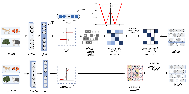
\includegraphics[width=0.95\textwidth]{papers_img/comparision_D2H_final.pdf}
    \caption{Comparison between deep learning for hashing and classification}
    \label{Fig:comparison_classification_vs_hash}
        \vspace{-4ex}
\end{figure*}
%\subsection{Motivation of nonlinear composite problem in deep hashing}
\subsection{Contributions}
In this paper, we propose an efficient deep hashing algorithm to address these challenges posed by nonlinear composition with W-type regularization. Our approach presents a reformulation of the W-type regularized problem using a decouple scheme and designs a new primal-dual algorithm using Fenchel duality. We aim to bridge the theoretical-practical gap by providing rigorous non-asymptotic convergence analysis and enhanced practical performance in deep hashing. Our main contributions are as follows:
\begin{itemize}[leftmargin=2em]
\item We reformulate deep hashing models with the W-type regularization into a two-block finite-sum optimization problem. This reformulation decouples the challenging $h(\bD(\bx))$, simplifying the sequential analysis.
\item Building on this problem, we propose \textbf{DualHash}, a stochastic primal-dual deep hashing algorithm. Using Fenchel duality, we partially transform the nonconvex W-type regularization optimization into a convex dual formulation that admits closed-form updates, ensuring robustness and stable convergence. To incorporate numerical acceleration, we develop two important instances: a momentum-based implementation (\textbf{DualHash-StoM}) and a variance-reduced implementation using StoRM (\textbf{DualHash-StoRM}).
\item We provide rigorous non-asymptotic complexity analysis for deep hashing optimization. Specifically, we establish an $\mathcal{O}(\varepsilon^{-4})$ complexity bound for DualHash-StoM and an improved optimal $\mathcal{O}(\varepsilon^{-3})$ complexity bound for DualHash-StoRM. Table~\ref{Table: summary of deep hashing algorithms} summarizes how our work compares to previous deep hashing methods. 
\item Extensive experiments on three standard datasets demonstrate the practical effectiveness of DualHash. In particular, our proposed method achieves consistently lower quantization errors across different bit lengths compared to baselines, validating the advantages of our primal-dual framework.
\end{itemize}

\begin{table}[t]
    \centering
    \caption{Comparison of optimization and convergence guarantee of deep hashing methods.}
    \label{Table: summary of deep hashing algorithms}
    \resizebox{\textwidth}{!}{
\begin{tabular}{cccccc}
\toprule
\textbf{Type} & \textbf{Method} & \textbf{Model} 
  & \textbf{Quantization Loss} & \textbf{Optimization} & \textbf{Complexity} \\
\midrule
    \multirow{3}{*}{\centering Discrete} 
    & DDSH \cite{liDeepSupervisedHashing} & $\min L_s(\bb) + Q(\bu, \bb)$ & \centering $\|\cdot\|^2$ & BQP & \multirow{12}{*}{\centering ---} \\
    \cmidrule(lr){2-5}
    & DSDH \cite{li2017deep}& \multirow{2}{*}{\centering $\min L_s(\bu) + Q(\bu, \bb)$} & \multirow{2}{*}{\centering $\|\cdot\|^2$} & $sgn$ update &  \\ 
    & DPSH \cite{liFeatureLearningBased2016} & &  & DCC &  \\ 
    \cmidrule(lr){1-5}
    \multirow{9}{*}{\centering Continuous}
    & DCH \cite{caoDeepCauchyHashing2018} &\multirow{4}{*}{\centering $\min L_s(\bu) + h(\bu)$} & $\log \left( 1 + \frac{\text{dist}_{\text{h}}(|\bu|, \mathbf{1})}{\gamma} \right)$ & \multirow{4}{*}{\centering SGDM} &  \\
    & DNNH \cite{laiSimultaneousFeatureLearning2015} & & $\mathcal{I}_{[-1,1]^d}(\bu)$ & &  \\
    & DSH \cite{liuDeepSupervisedHashing} & & $\| | \bu| - \mathbf{1}\|_1$ &  &  \\ 
    & DTSH \cite{wang2016DTSH} & & $\| | \bu| - \mathbf{1}\|_2^2$ &  &  \\ 
    & DHN \cite{zhuDeepHashingNetwork2016} & & $\sum_i\log(\cosh(|u_i|-1))$&  &  \\ 
    \cmidrule(lr){2-5}
    & MDSHC \cite{wang2023deep} & \scriptsize $\min L_c(\bu) + L_s (\bu)+ h(\bu)$ & $\| | \bu| - \mathbf{1}\|_1$ & RMSProp &  \\ 
    \cmidrule(lr){2-5}
    & HashNet \cite{Cao2017HashNetDL} & \multirow{2}{*}{\centering $\min L_s(\bu)$} & \multirow{2}{*}{\centering -} & SGDM &  \\     
    & OrthoHash \cite{hoeOneLossAll2021} & & & Adam &  \\
    % \cmidrule(lr){2-5}
    % & SBPG \cite{wang2024bregman} & \scriptsize $\min L_s(\bu) + h(\bu)$ & Weakly convex $h$ & SBregman PG & $\mathcal{O}(\varepsilon^{-4})$ \\
    \cmidrule(lr){2-6}
   & \textbf{DualHash-StoM} & \multirow{2}{*}{\small $ \min L_s(\bu) + Q(\bu,\bb) + h(\bb)$} & \multirow{2}{*}{$\| | \bb| - \mathbf{1}\|_1$} & \multirow{2}{*}{Sto Primal-Dual} & $\mathcal{O}(\varepsilon^{-4})$ \\
    & \textbf{DualHash-StoRM} & & & & $\mathcal{O}(\varepsilon^{-3})$ \\
    \bottomrule
    \end{tabular}
    }
    % \vspace{-5pt}
    \parbox{\textwidth}{\scriptsize
    \textbf{Notes}: 
    % The \textbf{Type} column indicates whether the method uses discrete or continuous optimization for quantization.
    The \textbf{Model} column shows the core optimization objective, where \(\bb\) denotes binary codes and \(\bu\) denotes continuous outputs. The \textbf{Quantization Loss} column specifies the loss (\(Q(\cdot, \cdot)\) or \(h(\cdot)\)) for quantization error, with `-' indicating no explicit loss. 
    % The \textbf{Optimization} column describes the training strategy, with discrete methods focusing on binary code updates. 
    DCC stands for Discrete Cyclic Coordinate, while BQP denotes Binary Quadratic Programming. The \textbf{Complexity} column reports the convergence rate, with `-' indicating no such analysis.
    }
     \vspace{-4ex}
\end{table}
\subsection{Related Work}
\label{Section: related work}
{We situate our contributions by reviewing related work on optimization in deep hashing, stochastic nonconvex constrained optimization, and primal-dual methods for structured composite problems.}

\paragraph{Optimization in Deep Hashing}
Improving retrieval accuracy and reducing the discrepancy between continuous representations and binary hash codes have long been central issues in deep hashing. One line of work adopts continuous relaxation and introduces explicit quantization regularization on network outputs; in particular, W-type regularizers such as $\||\mathbf{u}|-\mathbf{1}\|_1$ have been widely used to encourage binary-like activations \cite{liuDeepSupervisedHashing,wang2023deep,zhuDeepHashingNetwork2016}. Another line refines the discretization objective through greedy coding schemes, central similarity targets, or proxy-based supervision \cite{su2018greedy,yuanCentralSimilarityQuantization2020,MPDH2024,semanticHashCenters2025}. Alternative strategies directly address binary constraints by introducing auxiliary hash codes \cite{liDeepSupervisedHashing,li2017deep,liFeatureLearningBased2016}. Notably, even recent architectures retain W-type regularization; for instance, \cite{he2025mambahash} employs $\||\mathbf{u}|-\mathbf{1}\|_2^2$ as a smooth surrogate for $\||\mathbf{u}|-\mathbf{1}\|_1$ to facilitate gradient-based optimization, indicating that the practical relevance of W-type regularization has not diminished. The remaining challenge is to develop theoretically grounded optimization methods that can directly handle nonsmooth W-type regularization under nonlinear deep network mappings, which is precisely the focus of this work.
% Recent studies have further strengthened backbone architectures to improve feature quality, extending deep hashing from conventional CNNs to hybrid CNN--Transformer frameworks \cite{he2024hybridhash}, Transformer-based hashing models \cite{chen2021transhash,wu2025fth,liu2025capmh}, and state-space architectures \cite{he2025mambahash}. 
\paragraph{Stochastic Nonconvex Constrained Optimization}
{From a constrained optimization perspective, Problem~\eqref{Eq: the general nonlinear composite problem in intro} can be reformulated as a nonlinearly constrained optimization problem of the form}
\[
  \min_{x}\; f(x) + h(x) \quad \text{s.t.}\quad c(x) = 0.
\]
\blue{Several recent works have established oracle complexity results for first-order stochastic augmented-Lagrangian and penalty methods for problems of this type.} \cite{jin2022stochastic} proposed a single-loop stochastic primal-dual method based on a linearized augmented-Lagrangian function, achieving oracle complexities of $\mathcal{O}(\varepsilon^{-6})$ from an arbitrary initial point and $\mathcal{O}(\varepsilon^{-5})$ from a feasible one for locating an $\varepsilon$-KKT point. By incorporating the recursive momentum estimator of \cite{cutkoskyMomentumBasedVarianceReduction2019}, \cite{shi2025momentum} developed a momentum-based linearized augmented-Lagrangian method, improving these bounds to $\mathcal{O}(\varepsilon^{-4})$, or the nearly optimal $\mathcal{O}(\varepsilon^{-3})$ when initialized at a nearly feasible point. To certify a stronger notion of stationarity that deterministically enforces constraint violation of at most $\varepsilon$, \cite{lu2024variancereducedfirstordermethodsdeterministically} introduced a linearized quadratic-penalty method with truncated momentum. Under a regularity condition on the constraint gradients, recursive momentum yields the nearly optimal complexity $\widetilde{\mathcal{O}}(\varepsilon^{-3})$. 
% while Polyak momentum with diminishing step sizes achieves $\widetilde{\mathcal{O}}(\varepsilon^{-4})$.
\paragraph{Primal-Dual Methods for Structured Composite Problems}
In imaging science, the Primal-Dual Hybrid Gradient (PDHG) method \cite{chambolleFirstOrderPrimalDualAlgorithm2011} establishes an ergodic $\mathcal{O}(1/k)$ convergence rate for the primal-dual gap in convex settings and has found broad application in imaging inverse problems. \cite{esserZhangChan2010} proposed a unified framework for a broad class of first-order primal-dual algorithms for convex imaging problems, also achieving $\mathcal{O}(1/k)$ ergodic convergence. The stochastic extension, SPDHG \cite{chambolleSPDHG2018}, establishes almost-sure convergence and ergodic $\mathcal{O}(1/k)$ guarantees for structured finite-sum composite objectives under arbitrary sampling. \cite{chouzenouxAdjointMismatch} further showed that primal-dual methods retain convergence in the presence of adjoint mismatch, a perturbation closely related to stochastic gradient approximations; \cite{chouzenouxStochasticMM2017} developed a stochastic majorize-minimize subspace algorithm for online penalized estimation with rigorous convergence guarantees in imaging reconstruction settings. Extending to nonconvex settings, \cite{clasonAccelerationGlobalConvergence2019} established global convergence of a first-order primal-dual method under the Kurdyka--{\L}ojasiewicz condition. For nonconvex composite finite-sum objectives, \cite{guo2023preconditioned} proposed preconditioned primal-dual gradient methods with convergence analysis, while \cite{tran2022hybrid} developed a hybrid stochastic framework achieving $\mathcal{O}(\varepsilon^{-4})$ complexity. When the problem admits a block-separable structure, ADMM provides a natural decomposition framework; nonconvex ADMM convergence has been systematically established \cite{li2015global,hong2016convergence,wangGlobalConvergenceADMM2018,boct2020proximal}, and \cite{huang2019faster} established an $\mathcal{O}(\varepsilon^{-4})$ sample complexity bound for the nonconvex stochastic case. {However, the above results either rely on convex or linearly coupled structures, or address only single-block stochastic updates; the multi-block, nonconvex, nonlinearly coupled stochastic setting arising in deep hashing remains largely unaddressed.}

\section{Preliminary}
The extended real-valued function $f: \mathbb{R}^{q}\rightarrow (-\infty, +\infty]$ is called \textit{proper} if its domain $\text{dom}(f) := \{\bx \in \calX\mid f(\bx) < +\infty\}$ is nonempty and $\inf\limits_{\bx \in \mathbb{R}^q}f > -\infty$; it is \textit{closed} if its epigraph $\text{epi}(f) := \left\{ (\bx, t) \in \mathbb{R}^{q+1}\mid f(\bx) \leq t \right\}$ is closed.  For a proper, closed, and convex function $f$, the \textit{proximal mapping} of $f$, denoted by $\operatorname{prox}_{\tau f}(\by)$, is defined as
\begin{align}
    % \label{Def: the definition of proximal operator}
    \operatorname{prox}_{\tau f}(\by) := \argmin\limits_{\bx \in \operatorname{dom}(f)}\left\{ f(\bx) + \frac{1}{2\tau}\|\bx - \by\|^{2}\right\}, \notag
\end{align} 
where $\tau$ is a positive scalar parameter. The proximal mapping admits the following
properties.
\begin{proposition}[\cite{Rockafellar1998VariationalA}]
    Let $f : \mathbb{R}^{q}\rightarrow \mathbb{R}\cup \{+\infty\}$ be proper and
    closed. Then, the following holds.
    \begin{enumerate}[label=(\roman{*})]
        \item The set $\operatorname{prox}_{\tau f}(\bx)$ is nonempty and compact
            for any $\bx \in \mathbb{R}^{q}$ and $\tau > 0$.

        \item If $f$ is convex, then $\operatorname{prox}_{\tau f}(\bx)$
            contains exactly one value for any $\bx \in \mathbb{R}^{q}$ and
            $\tau > 0$.
    \end{enumerate}
\end{proposition}

Let us introduce the StoRM (Stochastic Recursive Momentum) variance reduction estimator \cite{cutkoskyMomentumBasedVarianceReduction2019}. In stochastic optimization problems where $F(\bx) = \mathbb{E}_{\xi}[F(\bx;\xi)]$ with $\xi \in \Xi$, 
% standard momentum methods use
% \begin{align*}
%     \bd^{k}= \rho_{k}\nabla F(\bx^{k}, \xi^{k}) + (1 - \rho_{k}) \bd^{k-1}, \text{ where }\rho_{k}\in [0, 1],
% \end{align*}
% yielding a biased estimate of $\nabla F(\bx^{k})$.
StoRM adds a
correction term, $(1 - \rho_{k}) (\nabla F(\bx^{k}, \xi^{k}) - \nabla F(\bx^{k-1}, \xi^{k}))$, resulting in:
\begin{align*}
     & \bd^{k}=\left\{\begin{array}{ll}\nabla F\left(\bx^{k}, \xi^{k}\right), & \text{if } k=1, \\ \nabla F\left(\bx^{k}, \xi^{k}\right) + \left(1-\rho_k\right)\left( \bd^{k-1} - \nabla F\left(\bx^{k-1}, \xi^{k}\right) \right), & \text{if } k>1,\end{array}\right. \\
     & \bx^{k+1}=\bx^{k}-\eta_{k}\bd^{k}.
\end{align*}
This exploits the smoothness of $F(\cdot, \xi)$, leading to efficient
variance reduction. When $\rho_{k}= 1$, $\bd^{k}$ reduces to vanilla mini-batch SGD. We set $\rho_{k}\in (0,1)$ for $k \geq 1$ in this paper

A function $f: \calX \rightarrow \RR$ is said to be $L_f$-smooth if  $\| \nabla f(\bx) - \nabla f(\bx') \| \leq L_f \| \bx - \bx'\|$ for all $\bx,\, \bx' \in \RR^n$. A mapping $\mathcal{M} : \mathcal{D} \to \RR^l $ is said to be $C$-Lipschitz continuous if $\|\mathcal{M}(\bx) - \mathcal{M}(\bx')\| \leq C\|\bx - \bx'\|$ for all $\bx, \bx' \in \mathcal{D}$. 

% A well-known gradient descent lemma for a smooth function is that
% \begin{align}
% % \label{Eq: the descent lemma}
%     f(\bx) \leq f(\bx') + \langle \nabla f(\bx'), \bx - \bx' \rangle + \frac{L_f}{2} \| \bx - \bx'\|^2. \notag
% \end{align}

% \section{Problem reformulation}
% \label{Section: Problem Reformulation}
% \subsection{W-type Regularized Deep Hashing Model}
% Deep hashing methods aim to learn network parameters \(\bx \in \calX \subseteq \RR^{d_{\bx}}\) to generate discrete codes that preserve semantic similarity effectively in the Hamming space. 
% A natural approach is to minimize a similarity-preserving loss function \( \frac{1}{n}\sum_{i=1}^n L_s(\text{sgn}(\bC_i(\bx)))\) where $n$ is the number of training samples, $\bC_i(\bx)$ represents the \(i\)-th network output and \(f_i\) is the similarity-preserving loss function (e.g., pairwise cross-entropy loss \cite{zhuDeepHashingNetwork2016}). However, the function \( sgn(\cdot) \) renders standard backpropagation infeasible due to its zero gradient for all nonzero inputs. This discreteness poses a central challenge in deep hashing.

% A W-type regularization (e.g., $\lambda | |z| - 1 |$) has effectively mitigated this issue. This type of regularization encourages outputs to approach binary values \(\{-1, 1\}\) during training. Specifically, the model is trained to produce continuous outputs \(\bu_i = \bD_i(\bx)\) with W-type regularization, and binary codes are obtained post-training via \(\bb_i = \text{sgn}(\bu_i)\).  Consequently, we formulate the core optimization problem for W-type regularized deep hashing methods as follows,
% \begin{align}
% \label{Eq: the primal deep hashing problem}
% \min_{\bx \in \calX} \quad \frac{1}{n} \sumn f_i (\bx) + \sumn h(\bD_i(\bx)), 
% \end{align}where \(\frac{1}{n}\sumn f_i\) is the similarity-preserving loss, \(D_i\) is the \(i\)-th network output and \(h\) is a W-type regularization.
% % \footnote{In the problem \eqref{Eq: the primal deep hashing problem}, we use vectorized \(\bz\), thus the regularization is also \(\| |\bz| - \bm{1}\|_1 = \sumn | |z_i| - 1 |\)}.
% \subsection{A Two-Block Structured Reformulation}
% We then employ variable splitting % \cite{wangLiftedBregmanTraining2022, zengBlockCoordinateDescent2018, lauProximalBlockCoordinate2018}, ]\
% to reformulate problem \eqref{Eq: the primal deep hashing problem} equivalently as the constrained problem:
% \begin{align} 
% \label{Eq: constrained_dlh} 
% \min_{\bx \in \mathcal{X}, \bB \in \mathcal{B}}&\quad \frac{1}{n} \sumn f_i (\bx) + \sum_{i=1}^n h(\bb_i) \notag \\ 
% \text{s.t.} &\quad \bb_i = \bD_i(\bx), \; \forall i=1,\dots,n. 
% \end{align} Combined with the quadratic penalty method \cite{nocedal1999numerical}, this transformation yields the following two-block finite-sum optimization problem:
% \begin{align} 
% \label{Prop: block-wise regularized problem} 
% \nonumber&\min_{\bx \in \mathcal{X}, \bB \in \mathcal{B}} J(\bx, \bB) \\
% &= \overbrace{\underbrace{\frac{1}{n}\sum_{i=1}^n f_i(\bx)}_{f(\bx)} + \underbrace{\frac{\gamma}{2n} \sum_{i=1}^n \| \bD_i(\bx) - \bb_i\|^2}_{P(\bx, \bB)}}^{F(\bx, \bB) = \frac{1}{n}\sumn F_i(\bx, \bb_i)} + \underbrace{\sum_{i=1}^n h(\bb_i)}_{h(\bB)}. \tag{P}
% \end{align} Here, \( \bB = [\bb_1, \bb_2, \dots, \bb_n]\) and \( \gamma > 0 \) is the penalty parameter. This reformulation decomposes the original problem \eqref{Eq: the primal deep hashing problem} into simpler structural blocks, enabling us to exploit the problem structure better. Building upon this problem, we develop a stochastic primal-dual algorithm that effectively addresses the challenges above.
\section{Problem reformulation}
\label{Section: Problem Reformulation}
\subsection{W-type Regularized Deep Hashing Model}
Deep hashing methods aim to learn network parameters \(\bx \in \calX \subseteq \RR^{d_{\bx}}\) to generate discrete codes that preserve semantic similarity effectively in the Hamming space. 
A natural approach is to minimize a similarity-preserving loss function \( \frac{1}{n}\sum_{i=1}^n L_s(\text{sgn}(\bC_i(\bx)))\) where $n$ is the number of training samples, $\bC_i(\bx)$ represents the \(i\)-th network output and \(f_i\) is the similarity-preserving loss function (e.g., pairwise cross-entropy loss \cite{zhuDeepHashingNetwork2016}). However, the function \( sgn(\cdot) \) renders standard backpropagation infeasible due to its zero gradient for all nonzero inputs. This discreteness poses a central challenge in deep hashing.

A W-type regularization (e.g., $\lambda | |z| - 1 |$) has effectively mitigated this issue. This type of regularization encourages outputs to approach binary values \(\{-1, 1\}\) during training. Specifically, the model is trained to produce continuous outputs \(\bu_i = \bD_i(\bx)\) with W-type regularization, and binary codes are obtained post-training via \(\bb_i = \text{sgn}(\bu_i)\).  Consequently, we formulate the core optimization problem for W-type regularized deep hashing methods as follows,
\begin{align}
    \label{Eq: the primal deep hashing problem}
    \min_{\bx \in \calX} \quad \frac{1}{n} \sumn f_i (\bx) + \sumn h(\bD_i(\bx)),
\end{align}
where \(\frac{1}{n}\sumn f_i\) is the similarity-preserving loss, \(D_i\) is the \(i\)-th network output and \(h\) is a W-type regularization.
\subsection{A Two-Block Structured Reformulation}
We then employ variable splitting to reformulate problem \eqref{Eq: the primal deep hashing problem} equivalently as the constrained problem:
\begin{align}
    % \label{Eq: constrained_dlh}
    \min_{\bx \in \mathcal{X}, \bB \in \mathcal{B}} \quad & \frac{1}{n} \sumn f_i (\bx) + \sum_{i=1}^n h(\bb_i) \notag \\
    \text{s.t.} \quad & \bb_i = \bD_i(\bx), \; \forall i=1,\dots,n. \notag
\end{align}
Combined with the quadratic penalty method \cite{nocedal1999numerical}, this transformation yields the following two-block finite-sum optimization problem:
\begin{align}
    \label{Prop: block-wise regularized problem}
    \min_{\bx \in \mathcal{X}, \bB \in \mathcal{B}} J(\bx, \bB) = \overbrace{\underbrace{\frac{1}{n}\sum_{i=1}^n f_i(\bx)}_{f(\bx)} + \underbrace{\frac{\gamma}{2n} \sum_{i=1}^n \| \bD_i(\bx) - \bb_i\|^2}_{P(\bx, \bB)}}^{F(\bx, \bB) = \frac{1}{n}\sumn F_i(\bx, \bb_i)} + \underbrace{\sum_{i=1}^n h(\bb_i)}_{h(\bB)}. \tag{P}
\end{align}
Here, \( \bB = [\bb_1, \bb_2, \dots, \bb_n]\) and \( \gamma > 0 \) is the penalty parameter. This reformulation decomposes the original problem \eqref{Eq: the primal deep hashing problem} into simpler structural blocks, enabling us to exploit the problem structure better. 
Building upon Problem~\eqref{Prop: block-wise regularized problem}, we develop a stochastic primal-dual algorithm \blue{that addresses the lack of tractable proximal mappings in the nonsmooth composite form and the absence of convergence guarantees in existing deep hashing methods.}

% \section{Algorithm}
% \label{Section: Methodology}
% \subsection{DualHash: A Stochastic Primal-Dual Hashing Algorithm}
% Inspired by PDHG \cite{chambolleFirstOrderPrimalDualAlgorithm2011} in convex optimization and its nonconvex extension PPDG \cite{guoPreconditionedPrimalDualGradient2023}, we consider the equivalent constrained formulation of  the problem \eqref{Prop: block-wise regularized problem}:
% \begin{align} 
% \min_{\bx \in \mathcal{X}, \bB \in \mathcal{B}, \by \in \mathcal{Y}} &\quad F(\bx, \bB) + h(\bY) \notag \\
% \text{s.t. } &\quad \bY = \bB \nonumber ,
% \end{align} whose corresponding dual problem is 
% \begin{align}
% \label{Prop: the dual problem}
% \max_{\bLmbd \in \mathcal{Y}^*} \min_{\bx \in \mathcal{X}, \bB \in \mathcal{B}, \by \in \mathcal{Y}} &\quad F(\bx, \bB) + h(\bY) + \langle \bLmbd, \bB - \bY \rangle. \tag{D}
% \end{align} 
% Recalling the definition of the conjugate function \cite{Rockafellar1998VariationalA}:
% \begin{equation}
% \label{eq:fenchel_conjugate}
% h^*(\bY) := \sup_{\bx \in \mathcal{Y}} \{ \langle \bY, \bx \rangle - h(\bx) \}, \quad \bY \in \mathcal{Y}^*
% \end{equation} and observing that the minimization with respect to $\bY$ in the problem \eqref{Prop: the dual problem} can be performed independently, we then simplify the Lagrangian function in the problem \eqref{Prop: the dual problem} to 
% \begin{align}
% \label{Eq: simplified_lagrangian}
% \calL(\bx, \bB, \bLmbd) := F(\bx, \bB) + \langle \bB, \bLmbd \rangle - h^*(\bLmbd).\tag{\(\calL\)}
% \end{align}

% Through this transformation, we replace $h(\bY)$ with $-h^*(\bLmbd)$ and can optimize \(h^*\) in the dual space. Since $h^*$ is always convex and l.s.c. \cite{Rockafellar1998VariationalA}, it means that the $\text{prox}_{h^*}(\cdot)$ is often much easier to compute (potentially having a closed-form solution) than that of $h$.  For $h(\bz) = \sum_{i=1}^n \lambda ||z_i| - 1|$, we derive its conjugate function as illustrated in \Cref{fig:w_type_regularization}:
% \begin{align*}
% &h^*(\bx) = \sum_{i=1}^n h^*(x_i),\,\, \notag \\
% & \text{where } h^*(x_i) = \begin{cases}
%     |x_i|, & \text{if } x_i \in [-\lambda, \lambda],\\
%     +\infty, & \text{otherwise},
%     \end{cases}
% \end{align*} whose proximal operator  in the piecewise solution is 
% \begin{align}
%     \label{Eq: the proximal mapping of conjugate function}
%     [\operatorname{prox}_{\tau h^*}(\by)]_i = 
%     \begin{cases}
%         \lambda, & y_i > \lambda +\tau,\\
%         y_i -\tau, & \tau < y_i \leq \lambda +\tau, \\
%         0, & -\tau \leq y_i \leq\tau, \\
%         y_i +\tau, &  - \lambda -\tau \leq y_i < -\tau, \\
%         -\lambda, & y_i < -\lambda -\tau.
%     \end{cases}
% \end{align} This motivates us to perform a proximal step to update \(\bLmbd\).
% \begin{figure}[!t]
% \centering
% \includegraphics[width=\columnwidth]{papers_img/W_type_with_its_conjugate_func.pdf}
% \caption{W-type regularization function $h(z) = \lambda ||z| - 1|$ and its conjugate function $h^*(x)$.}
% \label{fig:w_type_regularization}
% \vspace{-1ex}
% \end{figure} We now outline \textbf{DualHash}, which employs an alternating update scheme for $\bx, \bB, \bm{\Lambda}$. 
% we adopt a stochastic first-order method for the $\bx$-update since computing the full gradient \( \nabla_{\bx} F(\bx, \bB) \) is computationally expensive for typically the large number of samples $n$ in deep learning. Specifically, at each iteration $k$, we uniformly sample a mini-batch \(\calJ_k \subseteq \{1,\cdots,n\}\) with \(b_k = |\calJ_k| \leq n\) and compute:
% \begin{align}
% \label{Eq: the mini batch stochastic gradient estimator of F at x}
% \nabla_{\bx} F(\bx^k, \bB^k; \calJ_k)
% =\, \frac{1}{|\mathcal{J}_k|}\sum_{j \in \mathcal{J}_k} \nabla_{\bx} F_j(\bx^k, \bb_j^k).
% \end{align}
% Then we utilize this approximation within an optimization strategy chosen to enhance efficiency (e.g., incorporating momentum or variance reduction), as detailed in \Cref{Sec: Algorithm implementations}.
% Second, the auxiliary variable $\bB$ is updated via a simple gradient descent step \eqref{Eq: the update of B}; this suffices because the objective \eqref{Eq: simplified_lagrangian} with respect to $\bB$ is smooth with an inexpensive gradient, 
% % which is slightly different from \cite{chambolleFirstOrderPrimalDualAlgorithm2011}:
%     \begin{align}
%    \nonumber \bB^{k+1} &= \bB^k - \tau \nabla_{\bB}\calL(\bx^{k+1}, \bB^k, \bLmbd^k)\\
%     &= \bB^k - \tau \left( \nabla_{\bB} F(\bx^{k+1}, \bB^k) + \bLmbd^k \right). \label{Eq: the update of B}
%     \end{align}
%     Finally, the dual variable $\bLmbd$ is updated via proximal gradient ascent on $h^*$, using an extrapolation step introduced in \cite{chambolleFirstOrderPrimalDualAlgorithm2011}. The update solves the following optimization problem:
% \begin{align}
%     \bLmbd^{k+1} &= \text{prox}_{(1/\tau h^*)} \left( \bLmbd^k + \left(2\bB^{k+1} - \bB^k  \right) \right) \notag \\
%     &=  \arg\min_{\bLmbd \in \mathcal{Y}^* } \left\{ h^*(\bLmbd) - \langle \bLmbd, 2\bB^{k+1} - \bB^k \rangle \right. \notag \\
%     &\quad\quad\quad\quad\quad\quad\quad\quad\quad\quad\left. + \frac{\tau}{2} \| \bLmbd - \bLmbd^k\|^2 \right\}. 
%     \label{Eq: the update of lambda}
% \end{align}
% \subsection{Implementations}
% \label{Sec: Algorithm implementations}
% The unified DualHash framework allows for flexible choices in the $\bx$ update step based on a mini-batch stochastic gradient approximation \eqref{Eq: the mini batch stochastic gradient estimator of F at x}. This flexibility enables us to incorporate advanced stochastic optimization techniques. We thus instantiate the $\bx$-update using two well-established approaches: \textbf{momentum} \cite{Nesterov1983AMF, Polyak1964} and \textbf{variance reduction} \cite{driggs2022biased}, which can improve empirical training efficiency and can also improve the theoretical convergence guarantees \cite{Liu2020AnIA,sutskever2013importance}.

% % \vspace{5pt}
% \paragraph{DualHash-StoM}
% %Numerically, 
% The heavy ball method \cite{Polyak1964} and Nesterov acceleration \cite{Nesterov1983AMF} can be integrated with stochastic gradient descent (SGD) to yield accelerated variants like SGD with momentum, which significantly speeds up convergence.
% This approach has become a popular strategy for training neural networks \cite{fotopoulos2024review,Hertrich2020InertialSP}. We thus incorporate this technique and compute the stochastic gradient estimator (Line 3 of \Cref{alg:our_algorithm_sgdm}) as:
% \begin{align}
% \label{Eq: the stochastic approximate in SGDM}
%     \bG^k = \nabla_{\bx} F(\bz^k, \bB^k; \calJ_k),\, \text{where } \bz^k = \bx^k + \beta_k (\bx^k - \bx^{k-1}).
% \end{align} The update of \( \bx^k\) (Line 4 of Alg. \ref{alg:our_algorithm_sgdm}) is then:
% \begin{align}
% \label{Eq: the update of x in SGDM}
%     \bx^{k+1} = \by^k - \eta_k \bG^k,\,\text{where } \by^k = \bx^k + \alpha_k (\bx^k - \bx^{k-1}). 
% \end{align} The overall algorithm, DualHash-StoM, is detailed in \Cref{alg:our_algorithm_sgdm}.
% \begin{remark}
% The momentum acceleration framework in \eqref{Eq: the update of x in SGDM} covers these two accelerations:
% Nesterov acceleration \cite{Nesterov1983AMF} corresponds to $\alpha_k = \beta_k \neq 0$; the heavy-ball method \cite{Polyak1964} is obtained with $\beta_k = 0$; vanilla SGD is recovered when $\alpha_k = \beta_k = 0$; In this paper, we set $\alpha_k, \beta_k \in (0,1)$ for all $k \geq 1$. 
% \end{remark}

% % \vspace{3pt}
% \paragraph{DualHash-StoRM}
% Alternatively, we employ the STORM estimator \cite{cutkoskyMomentumBasedVarianceReduction2019} for the $\bx$-update. STORM utilizes a recursive momentum mechanism to reduce gradient variance, which is motivated by SGDM. Unlike some other variance reduction techniques (e.g., SVRG \cite{johnsonAcceleratingStochasticGradient2013}, SARAH \cite{SARAH2017}) that require full-gradient or large-batch gradient computations, STORM achieves variance reduction without such requirements. Given its practical effectiveness in deep learning \cite{cutkoskyMomentumBasedVarianceReduction2019,levy2021storm+}, we compute the stochastic gradient estimator (Line 3 of \Cref{alg:our_algorithm_storm}) as:
% % {\small
% % \begin{align}
% % \label{Eq: the stochastic approximate in STORM}
% % \bD^k =
% % \begin{cases} 
% % \nabla_{\bx} F(\bx^1, \bB^1; \calJ_1), & \text{if } k = 1, \\
% % \nabla_{\bx} F(\bx^k, \bB^k; \calJ_k) + (1 - \rho_{k-1}) \left( \bD^{k-1} - \nabla_{\bx} F(\bx^{k-1}, \bB^{k-1};\calJ_{k-1})\right), & \text{if }k > 1.
% % \end{cases}
% % \end{align}}
% {\small
% \begin{align}
% \label{Eq: the stochastic approximate in STORM}
% \bD^k =
% \begin{cases} 
% \nabla_{\bx} F(\bx^1, \bB^1; \mathcal{J}_1), &\text{if }  k = 1, \\
% (1 - \rho_{k-1}) \big( \bD^{k-1} - \nabla_{\bx} F(\bx^{k-1}, \bB^{k-1};\mathcal{J}_{k-1})\big)\\
% +\nabla_{\bx} F(\bx^k, \bB^k; \mathcal{J}_k), & \text{if } k > 1.
% \end{cases}
% \end{align}}
% The update of $\bx$ (Line 4 of \Cref{alg:our_algorithm_storm}) is then 
% \begin{align}
% \label{Eq: the update of x in STORM}
%     \bx^{k+1} = \bx^k - \eta_k \bD^k.
% \end{align} The overall algorithm, DualHash-StoRM, is detailed in \Cref{alg:our_algorithm_storm}.

% \begin{figure}[!htbp]
%     \vspace{-5mm} 
%     \begin{minipage}[t]{0.485\textwidth}
%         \begin{algorithm}[H]
%        \caption{DualHash-StoM}
%         \small   % 或使用 \footnotesize 更小
%         \setlength{\baselineskip}{0.8\baselineskip}  % 减少行间
%       \label{alg:our_algorithm_sgdm}
%       \begin{algorithmic}[1]
%         \STATE \textbf{Initialize:} $\bx^1 = \bz^1 = \by^1 \in \calX $, \( \bB^1 \in \calB,\, \bLmbd^1\in \calY^*\), parameters $\{\eta_k\} $, $\tau$, $b_k$, $\{\alpha_k, \beta_k \in (0,1)\}$
%         \FOR{$k = 1, 2, \ldots$}               
%           \STATE Compute \(\bG^k\) by \eqref{Eq: the stochastic approximate in SGDM}
%           \STATE Update $\bx^{k+1}$ by \eqref{Eq: the update of x in SGDM}
%           \STATE Update $\bB^{k+1}$ by \eqref{Eq: the update of B}
%           \STATE Update $\bm{\Lambda}^{k+1}$ by \eqref{Eq: the update of lambda}
%         \ENDFOR
%         \STATE \textbf{Return:} $\bx_R$ where $R$ is uniformly sampled from $\{2, \ldots, T+1\}$
%       \end{algorithmic}
%     \end{algorithm}
%   \end{minipage}
%   \hspace{0.5mm} 
%   \begin{minipage}[t]{0.485\textwidth}
%     \begin{algorithm}[H]
%         \caption{ DualHash-StoRM}
%       \small
%       \setlength{\baselineskip}{0.8\baselineskip}
%       \label{alg:our_algorithm_storm}
%       \begin{algorithmic}[1]
%         \STATE  \textbf{Initialize:} $\bx^1  \in \calX$, \( \bB^1 \in \calB,\, \bLmbd^1\in \calY^*\), parameters $\{\eta_k\} $, $\tau $, $b_k$, $\{\rho_k\in (0,1)\}$
%         \FOR{$k = 1, 2, \ldots$}
%         \STATE Compute $\bD^k$ by \eqref{Eq: the stochastic approximate in STORM}
%         \STATE Update $\bx^{k+1}$ by \eqref{Eq: the update of x in STORM}.
%         \STATE Update $\bB^{k+1}$ by \eqref{Eq: the update of B}.
%         \STATE Update $\bm{\Lambda}^{k+1}$ by \eqref{Eq: the update of lambda}.
%         \ENDFOR
%         \STATE \textbf{Return:} $\bx_R$ where $R$ is uniformly sampled from $\{2, \ldots, T+1\}$
%       \end{algorithmic}
%     \end{algorithm}
%   \end{minipage}
%   \vspace{-1ex}
% \end{figure}
% \begin{remark}
% The update steps for $\bB$ and $\bm{\Lambda}$ imply the following optimality conditions, which may result in explicit closed-solution in deep hashing. The $\bB$-update in \eqref{Eq: the update of B} yields:
% \begin{align}
%     \label{Eq: the optimality condition of Bk}
%     \bB^{k} = \bB^{k-1} - \tau \left( \nabla_{\bB}F(\bx^{k}, \bB^{k-1}) + \bm{\Lambda}^{k-1} \right).
% \end{align}
% For the $\bm{\Lambda}$-update in \eqref{Eq: the update of lambda}, the proximal operator definition gives:
% \[
%     \tau \left( \bm{\Lambda}^{k} + \tau^{-1}(2\bB^{k} - \bB^{k-1}) - \bm{\Lambda}^{k} \right) \in \partial h^{*}(\bm{\Lambda}^{k}),
% \]
% which is equivalent to the existence of $\mathcal{G}_{\bm{\Lambda}}^{k} \in \partial h^{*}(\bm{\Lambda}^{k})$ such that:
% \begin{align}
%     \label{Eq: the optimality condition of lbda}
%     \mathcal{G}_{\bm{\Lambda}}^{k} = (2\bB^{k} - \bB^{k-1}) + \tau(\bm{\Lambda}^{k-1} - \bm{\Lambda}^{k}).
% \end{align}
% If the sequence \(\{ (\bx^k, \bB^k, \bm{\Lambda}^k) \}\) converges to \((\bx^*, \bB^*, \bm{\Lambda}^*)\), then by the outer semicontinuity of $\partial h^{*}(\cdot)$, we have $\bB^* \in \partial h^*(\bm{\Lambda}^*)$.
% % which corresponds to the necessary condition \eqref{Eq: the sufficient and necessary condition for dual} for the second relation in optimality condition \eqref{Eq: the sufficient and necessary condition}.
% This establishes \eqref{Eq: the sufficient and necessary condition for dual}, which is precisely the necessary condition for the second relation in \eqref{Eq: the sufficient and necessary condition}.
% \end{remark}
\section{Algorithm}
\label{Section: Methodology}
\subsection{DualHash: A Stochastic Primal-Dual Hashing Framework}
Inspired by PDHG \cite{chambolleFirstOrderPrimalDualAlgorithm2011},
% and its nonconvex extension PPDG \cite{guoPreconditionedPrimalDualGradient2023}, 
we consider the equivalent constrained formulation of  the problem \eqref{Prop: block-wise regularized problem}:
\begin{align} 
\min_{\bx \in \mathcal{X}, \bB \in \mathcal{B}, \bY \in \mathcal{Y}} &\quad F(\bx, \bB) + h(\bY) \notag \\
\text{s.t. } &\quad \bY = \bB \nonumber ,
\end{align} whose corresponding dual problem is 
\begin{align}
\label{Prop: the dual problem}
\max_{\bLmbd \in \mathcal{Y}^*} \min_{\bx \in \mathcal{X}, \bB \in \mathcal{B}, \bY \in \mathcal{Y}} &\quad F(\bx, \bB) + h(\bY) + \langle \bLmbd, \bB - \bY \rangle. \tag{D}
\end{align} 
Recalling the definition of the conjugate function \cite{Rockafellar1998VariationalA}:
\begin{equation}
\label{eq:fenchel_conjugate}
h^*(\bY) := \sup_{\by \in \mathcal{Y}} \{ \langle \bY, \by \rangle - h(\by) \}, \quad \bY \in \mathcal{Y}^*
\end{equation} and observing that the minimization with respect to $\bY$ in the problem \eqref{Prop: the dual problem} can be performed independently, we then simplify the Lagrangian function in the problem \eqref{Prop: the dual problem} to 
\begin{equation}
\label{Eq: simplified_lagrangian}
\calL(\bx, \bB, \bLmbd) := F(\bx, \bB) + \langle \bB, \bLmbd \rangle - h^*(\bLmbd).
\end{equation}
Through this transformation, we replace $h(\bY)$ with $-h^*(\bLmbd)$ and optimize the \(h^*\) in the dual space. The convexity of $h^*$ makes $\operatorname{prox}_{h^*}(\cdot)$ often much easier to compute (potentially having a closed-form solution) than $\operatorname{prox}_{h}(\cdot)$.
For $h(\bz) = \sum_{i=1}^n \lambda ||z_i| - 1|$, we derive its conjugate function as illustrated in \Cref{fig:w_type_regularization}:
\begin{align*}
&h^*(\bx) = \sum_{i=1}^n h^*(x_i),\,\, \text{where } h^*(x_i) = \begin{cases}
    |x_i|, & \text{if } x_i \in [-\lambda, \lambda],\\
    +\infty, & \text{otherwise},
    \end{cases}
\end{align*} whose proximal operator in the piecewise solution is 
\begin{align}
    \label{Eq: the proximal mapping of conjugate function}
    [\operatorname{prox}_{\tau h^*}(\by)]_i = 
    \begin{cases}
        \lambda, & y_i > \lambda +\tau,\\
        y_i -\tau, & \tau < y_i \leq \lambda +\tau, \\
        0, & -\tau \leq y_i \leq\tau, \\
        y_i +\tau, &  - \lambda -\tau \leq y_i < -\tau, \\
        -\lambda, & y_i < -\lambda -\tau.
    \end{cases}
\end{align} This motivates us to perform a proximal step to update \(\bLmbd\).
\begin{figure}[t]
\centering
\includegraphics[width=0.6\textwidth]{papers_img/W_type_with_its_conjugate_func.pdf}
\caption{W-type regularization function $h(z) = \lambda ||z| - 1|$ and its conjugate function $h^*(x)$.}
\label{fig:w_type_regularization}
\vspace{-3 ex}
\end{figure}

We now outline the \textbf{DualHash} framework, which employs an alternating update scheme for $\bx, \bB, \bm{\Lambda}$. We adopt a stochastic first-order method for the $\bx$-update since computing the full gradient \( \nabla_{\bx} F(\bx, \bB) \) is computationally expensive for a typically large number of samples $n$ in deep learning. Specifically, at each iteration $k$, we uniformly sample a mini-batch \(\calJ_k \subseteq \{1,\cdots,n\}\) with \(b_k = |\calJ_k| \leq n\) and compute:
\begin{align}
\label{Eq: the mini batch stochastic gradient estimator of F at x}
\nabla_{\bx} F(\bx^k, \bB^k; \calJ_k)
=\, \frac{1}{|\mathcal{J}_k|}\sum_{j \in \mathcal{J}_k} \nabla_{\bx} F_j(\bx^k, \bb_j^k).
\end{align}
This formulation accommodates flexible stochastic gradient approximations, enabling the incorporation of advanced variance-reduction or momentum techniques, as detailed in \Cref{Sec: Algorithm implementations}.

Second, the auxiliary variable $\bB$ is updated via a vanilla gradient descent step \eqref{Eq: the update of B}; this suffices because the objective \eqref{Eq: simplified_lagrangian} with respect to $\bB$ is smooth with an inexpensive gradient, 
\begin{align}
   \nonumber \bB^{k+1} &= \bB^k - \tau \nabla_{\bB}\calL(\bx^{k+1}, \bB^k, \bLmbd^k)\\
    &= \bB^k - \tau \left( \nabla_{\bB} F(\bx^{k+1}, \bB^k) + \bLmbd^k \right). \label{Eq: the update of B}
\end{align}
Finally, the dual variable $\bLmbd$ is updated via proximal gradient ascent on $h^*$, using an extrapolation step introduced in \cite{chambolleFirstOrderPrimalDualAlgorithm2011}. The update solves the following optimization problem:
\begin{align}
    \bLmbd^{k+1} &= \text{prox}_{(1/\tau h^*)} \left( \bLmbd^k + \left(2\bB^{k+1} - \bB^k  \right) \right) \notag \\
    &=  \arg\min_{\bLmbd \in \mathcal{Y}^* } \left\{ h^*(\bLmbd) - \langle \bLmbd, 2\bB^{k+1} - \bB^k \rangle  + \frac{\tau}{2} \| \bLmbd - \bLmbd^k\|^2 \right\}. 
    \label{Eq: the update of lambda}
\end{align}

\subsection{Implementations}
\label{Sec: Algorithm implementations}
\paragraph{DualHash-StoM}
The heavy ball method \cite{Polyak1964} and Nesterov acceleration \cite{Nesterov1983AMF} has been extensively studied in large-scale nonconvex optimization \cite{gaoNonConvexStochasticComposite2024}.
Motivated by this, each iteration $k$,  we compute the stochastic gradient estimator (Line 3 of \Cref{alg:our_algorithm_sgdm}) as:
\begin{align}
\label{Eq: the stochastic approximate in SGDM}
    \bG^k = \nabla_{\bx} F(\bz^k, \bB^k; \calJ_k),\, \text{where } \bz^k = \bx^k + \beta_k (\bx^k - \bx^{k-1}).
\end{align} The update of \( \bx^k\) (Line 4 of Alg. \ref{alg:our_algorithm_sgdm}) is then:
\begin{align}
\label{Eq: the update of x in SGDM}
    \bx^{k+1} = \by^k - \eta_k \bG^k,\,\text{where } \by^k = \bx^k + \alpha_k (\bx^k - \bx^{k-1}). 
\end{align} The overall algorithm, DualHash-StoM, is detailed in \Cref{alg:our_algorithm_sgdm}.
\begin{remark}
The momentum acceleration framework in \eqref{Eq: the update of x in SGDM} covers these two accelerations: Nesterov acceleration corresponds to $\alpha_k = \beta_k \neq 0$; the heavy-ball method is obtained with $\beta_k = 0$; vanilla SGD is recovered when $\alpha_k = \beta_k = 0$. In this paper, we set $\alpha_k, \beta_k \in (0,1)$ for all $k \geq 1$. 
\end{remark}
\begin{algorithm}[t]
\caption{DualHash-StoM}
\label{alg:our_algorithm_sgdm}
\begin{algorithmic}[1]
\STATE \textbf{Initialize:} $\bx^1 = \bz^1 = \by^1 \in \calX $, \( \bB^1 \in \calB,\, \bLmbd^1\in \calY^*\), parameters $\{\eta_k\} $, $\tau$, $b_k$, $\{\alpha_k, \beta_k \in (0,1)\}$
\FOR{$k = 1, 2, \ldots$}               
  \STATE Compute \(\bG^k\) by \eqref{Eq: the stochastic approximate in SGDM}
  \STATE Update $\bx^{k+1}$ by \eqref{Eq: the update of x in SGDM}
  \STATE Update $\bB^{k+1}$ by \eqref{Eq: the update of B}
  \STATE Update $\bm{\Lambda}^{k+1}$ by \eqref{Eq: the update of lambda}
\ENDFOR
\STATE \textbf{Return:} $\bx_R$ where $R$ is uniformly sampled from $\{2, \ldots, T+1\}$
\end{algorithmic}
\end{algorithm}
\paragraph{DualHash-StoRM}
Alternatively, we employ the StoRM estimator \cite{cutkoskyMomentumBasedVarianceReduction2019} for the $\bx$-update. StoRM utilizes a recursive momentum mechanism to reduce gradient variance, which is motivated by SGDM. Unlike some other variance reduction techniques (e.g., SVRG \cite{johnsonAcceleratingStochasticGradient2013}, SARAH \cite{SARAH2017}) that require full-gradient or large-batch gradient computations, StoRM achieves variance reduction without such requirements. Given its practical effectiveness in deep learning \cite{cutkoskyMomentumBasedVarianceReduction2019,levy2021storm+}, we compute the stochastic gradient estimator (Line 3 of \Cref{alg:our_algorithm_storm}) as:
{\small
\begin{align}
\label{Eq: the stochastic approximate in STORM}
\bD^k =
\begin{cases} 
\nabla_{\bx} F(\bx^1, \bB^1; \mathcal{J}_1), &\text{if }  k = 1, \\
(1 - \rho_{k-1}) \big( \bD^{k-1} - \nabla_{\bx} F(\bx^{k-1}, \bB^{k-1};\mathcal{J}_{k-1})\big)+\nabla_{\bx} F(\bx^k, \bB^k; \mathcal{J}_k), & \text{if } k > 1.
\end{cases}
\end{align}}
The update of $\bx$ (Line 4 of \Cref{alg:our_algorithm_storm}) is then 
\begin{align}
\label{Eq: the update of x in STORM}
    \bx^{k+1} = \bx^k - \eta_k \bD^k.
\end{align} The overall algorithm, DualHash-StoRM, is detailed in \Cref{alg:our_algorithm_storm}.
\begin{algorithm}[t]
\caption{DualHash-StoRM}
\label{alg:our_algorithm_storm}
\begin{algorithmic}[1]
\STATE  \textbf{Initialize:} $\bx^1  \in \calX$, \( \bB^1 \in \calB,\, \bLmbd^1\in \calY^*\), parameters $\{\eta_k\} $, $\tau $, $b_k$, $\{\rho_k\in (0,1)\}$
\FOR{$k = 1, 2, \ldots$}
\STATE Compute $\bD^k$ by \eqref{Eq: the stochastic approximate in STORM}
\STATE Update $\bx^{k+1}$ by \eqref{Eq: the update of x in STORM}.
\STATE Update $\bB^{k+1}$ by \eqref{Eq: the update of B}.
\STATE Update $\bm{\Lambda}^{k+1}$ by \eqref{Eq: the update of lambda}.
\ENDFOR
\STATE \textbf{Return:} $\bx_R$ where $R$ is uniformly sampled from $\{2, \ldots, T+1\}$
\end{algorithmic}
\end{algorithm}

% \begin{remark}
% The update steps for $\bB$ and $\bm{\Lambda}$ imply the following optimality conditions, which may result in explicit closed-solution in deep hashing. The $\bB$-update in \eqref{Eq: the update of B} yields:
% \begin{align}
%     \label{Eq: the optimality condition of Bk}
%     \bB^{k} = \bB^{k-1} - \tau \left( \nabla_{\bB}F(\bx^{k}, \bB^{k-1}) + \bm{\Lambda}^{k-1} \right).
% \end{align}
% For the $\bm{\Lambda}$-update in \eqref{Eq: the update of lambda}, the proximal operator definition gives:
% \[
%     \tau \left( \bm{\Lambda}^{k} + \tau^{-1}(2\bB^{k} - \bB^{k-1}) - \bm{\Lambda}^{k} \right) \in \partial h^{*}(\bm{\Lambda}^{k}),
% \]
% which is equivalent to the existence of $\mathcal{G}_{\bm{\Lambda}}^{k} \in \partial h^{*}(\bm{\Lambda}^{k})$ such that:
% \begin{align}
%     \label{Eq: the optimality condition of lbda}
%     \mathcal{G}_{\bm{\Lambda}}^{k} = (2\bB^{k} - \bB^{k-1}) + \tau(\bm{\Lambda}^{k-1} - \bm{\Lambda}^{k}).
% \end{align}
% If the sequence \(\{ (\bx^k, \bB^k, \bm{\Lambda}^k) \}\) converges to \((\bx^*, \bB^*, \bm{\Lambda}^*)\), then by the outer semicontinuity of $\partial h^{*}(\cdot)$, we have $\bB^* \in \partial h^*(\bm{\Lambda}^*)$.
% This establishes \eqref{Eq: the sufficient and necessary condition for dual}, which is precisely the necessary condition for the second relation in \eqref{Eq: the sufficient and necessary condition}.
% \end{remark}
% \section{Complexity analysis}
% \label{Section: Convergence analysis}

% We now investigate the complexity analysis for DualHash-StoM (\Cref{alg:our_algorithm_sgdm}) and DualHash-StoRM (\Cref{alg:our_algorithm_storm}). Our objective is to find an approximate stochastic critical point of the Lagrangian function \eqref{Eq: simplified_lagrangian}, i.e., a point satisfying 
% \begin{equation}\label{equ:esp}
% \mathbb{E} [\text{dist}^2(\bm{0}, \partial \calL (\bx^*, \bm{B}^*, \bm{\Lambda}^* ))] \leq \varepsilon^2
% \end{equation}
% for a given \(\varepsilon > 0\). We assume in this paper the set \(
% \text{crit} \calL := \{(\bx^*, \bm{B}^*, \bm{\Lambda}^* ) \in \mathcal{X} \times \mathcal{B} \times \mathcal{Y^*}: \bm{0} \in \partial \mathcal{L}(\bx^*, \bm{B}^*, \bm{\Lambda}^*)\}
% \) is nonempty. This focus is standard in non-convex stochastic optimization analysis, as finding a global or even local minimizer for non-convex optimization problems is generally NP-hard. In particular, we can prove that a critical point of the Lagrangian function \eqref{Eq: simplified_lagrangian} is a first-order necessary optimal condition of problem \eqref{Prop: block-wise regularized problem} as follows. 

% \begin{lemma}
% \label{Lemma: Optimality condition}
%     Suppose that \(\min\limits_{\bx, \bB} \calL(\bx, \bB, \bLmbd) > -\infty\)  and \((\bx^*, \bB^*, \bLmbd^*)\) are the optimal solutions of the problem \eqref{Prop: block-wise regularized problem} and the problem \eqref{Prop: the dual problem}, respectively. Then, it holds that \((\bx^*, \bB^*, \bLmbd^*) \in \text{crit} \calL\), i.e., \(\bm{0} \in \partial \mathcal{L}(\bx^*, \bB^*, \bLmbd^*)\).
% \end{lemma} 
% \setcounter{proof}{0}
% \begin{proof}
%     According to \cite[Theorem 2.158]{temporary-citekey-11039},
%     $(\bx^{*}, \bm{B}^{*}, \bm{\Lambda}^{*})$ are optimal solutions to the
%     primal problem \eqref{Prop: block-wise regularized problem} and the dual problem
%     \eqref{Prop: the dual problem} if and only if:
%     \begin{align}
%         \label{Eq: the sufficient and necessary condition}
%         \begin{cases}(\bx^{*}, \bm{B}^{*}) \in \argmin\limits_{\bx \in \calX, \bm{B} \in \mathcal{B}}\mathcal{L}(\bx^{*}, \bm{B}^{*}, \bm{\Lambda}^{*}), \\ 0 = h(\bm{B}^{*}) + h^{*}(\bm{\Lambda}^{*}) - \langle \bm{\Lambda}^{*}, \bm{B}^{*}\rangle.\end{cases}
%     \end{align}

%     The first condition in \eqref{Eq: the sufficient and necessary condition} implies
%     that $\bm{0}$ belongs to the subdifferential of $\mathcal{L}$ with respect to
%     $(\bx, \bm{B})$ at $(\bx^{*}, \bm{B}^{*}, \bm{\Lambda}^{*})$. Since $\calL$
%     is continuously differentiable in $(\bx, \bm{B})$, we have
%     \begin{align}
%         \label{Eq: the sufficient and necessary condition for primal}\begin{cases}\bm{0}&= \nabla f(\bx^{*}) + \nabla_{\bx}G(\bx^{*}, \bm{B}^{*}),\\ \bm{0}&= \nabla_{\bB}G(\bx^{*}, \bm{B}^{*}) + \bm{\Lambda}^{*}.\end{cases}
%     \end{align}
%     For the second condition in \eqref{Eq: the sufficient and necessary condition},
%     by the definition of the conjugate function, if this equality holds, then $\bm
%     {\Lambda}^{*}$ is the optimal solution of $\sup \{ \left<\bb^{*}, \blmbd\right
%     > - h^{*}(\blmbd) \}$, i.e.,
%     \begin{align}
%         \label{Eq: the sufficient and necessary condition for dual}\bm{B}^{*}\in \partial h^{*}(\bm{\Lambda}^{*}).
%     \end{align}
%     Combining \eqref{Eq: the sufficient and necessary condition for primal} and \eqref{Eq: the sufficient and necessary condition for dual},
%     we obtain $\bm{0}\in \partial \mathcal{L}(\bx^{*}, \bm{B}^{*}, \bm{\bLmbd}^{*}
%     )$, completing the proof. 
%     %, which can be written explicitly as:
%     % \begin{align}
%     %     \label{Eq: necessary_condition_dual}
%     %     \begin{cases}
%     %         \bm{0} &= \nabla f(\bx^*) + \nabla_{\bx} G(\bx^*, \bm{B}^*),\\
%     %         \bm{0} &= \nabla_{\bB} G(\bx^*, \bm{B}^*) + \bm{\Lambda}^*,\\
%     %         \bm{0} &\in \bm{B}^* - \partial h^*(\bm{\Lambda}^*).
%     %     \end{cases}
%     % \end{align}
%     % This system of equations characterizes the critical points of $\mathcal{L}$, thus completing the proof.
% \end{proof}

% We then make the following assumptions generally used in stochastic optimization \cite{Ghadimi2013MinibatchSA,huangMiniBatchStochasticADMMs2019,xu2023momentum}.
% \begin{assumption} 
% \label{Ass: main assumptions}
% \begin{itemize}[leftmargin=2em]
%     \item[{(i)}] We assume that the sequences \( \{(\bx^k, \bm{B}^k, \bm{\Lambda}^k) \}_{k \in \NN} \) generated by Algorithms \ref{alg:our_algorithm_sgdm} and \ref{alg:our_algorithm_storm} are bounded. Moreover, the objective of  \eqref{Prop: block-wise regularized problem} is lower bounded by \(J^*\).
%     \item[{(ii)}] We assume that \(F(\bx, \bB)\) is $L_F$-smooth with respect to $(\bx, \bB)$, where $L_F = \mathcal{O}\left(1\right)$.
%     \item[{(iii)}] Suppose index $i \sim \text{Uniform}\{1, \ldots, n\}$.  For any \(\bB \in \calB\), there exists a constant $\sigma^2 \geq 0$ such that $\mathbb{E}_{i}[\nabla_{\bx} F_i(\bx, \bb_i)] = \nabla_{\bx} F(\bx, \bB)$ and $\mathbb{E}_{i}[\|\nabla_{\bx} F_i(\bx, \bb_i) - \nabla_{\bx} F(\bx, \bB)\|^2] \leq \sigma^2$. 
% \end{itemize}
% \end{assumption}
% \begin{remark}
% \begin{enumerate}[label=(\roman*), leftmargin=2em]
%     \item The boundedness in \Cref{Ass: main assumptions} (i) is maintained in practice for each variable:  $\bm{\Lambda}^k$ remains bounded due to its proximal update rule \eqref{Eq: the update of lambda} for $\bm{\Lambda}^k$ with the truncation property of $\text{prox}_{h^*}$ in \eqref{Eq: the proximal mapping of conjugate function}; The $\bB^k$ naturally converges toward $\pm 1$ through W-type regularization; and network parameters $\bx^k$ are stabilized via weight decay and pretrained initialization, ensuring objective coercivity.
%     \item The smoothness constant \(L_F\) remains \(\mathcal{O}(1)\), as the penalty formulation is designed to cancel the potential \(\mathcal{O}(\sqrt{n})\) scaling of individual components. A rigorous analysis is provided in Appendix C.
% \end{enumerate}
% \end{remark}
% Our analysis aims to bound \( \EE [\| \partial \calL\|^2]\). However, due to the existence of dual variables \(\bLmbd\), the Lagrangian function \eqref{Prop: the dual problem} lacks the descent property. This makes it difficult to apply standard approaches from prior work \cite{tran2022hybrid,wang2019spiderboost,xu2023momentum,zhang2022stochastic}, which often leverage the descent of their objective functions or corresponding potential functions. Instead, we shall construct an appropriate Lyapunov function. To enable this construction, we first analyze how to control the dual variable dynamics by establishing bounds on \(\|\bm{\Lambda}^{k+1} - \bm{\Lambda}^k \|^2\) with the primal variables residuals.
% \begin{lemma}
% \label{Lemma: dual boundedness}
% Under \Cref{Ass: main assumptions}, for \(k \geq 1 \), it holds that
%     \begin{align}
%        \nonumber
%         &\|\bm{\Lambda}^{k+1}- \bm{\Lambda}^k \|^2 \\
%         \leq&\, 3 \tau^{-2} \|\bB^{k+2} - \bB^{k+1}\|^2 + 3(\tau^{-1} + L_F)^2  \|\bB^{k+1} - \bB^{k}\|^2   \notag \\
%         &+ 3L_F^2  \|\bx^{k+2} - \bx^{k+1}\|^2.
%          \label{Eq: dual boundedness}
%     \end{align}
% \end{lemma}
% \begin{proof}
%     Using the update of $\bm{B}^{k}$ in \eqref{Eq: the update of B} twice yields
%     that
% \begin{align*}
%      & \|\bm{\Lambda}^{k+1}- \bm{\Lambda}^{k}\| \notag    \\
%         = &\,\left\| \tau^{-1}(\bm{B}^{k+1}- \bm{B}^{k+2}) + \tau^{-1}(\bm{B}^{k+1}- \bm{B}^{k}) \right. \\ 
%         & \left. \quad + \nabla_{\bB}F(\bx^{k+1}, \bm{B}^{k}) - \nabla_{\bB}F(\bx^{k+2}, \bm{B}^{k+1}) \right\| \\
%        \leq & \,\tau^{-1}\|(\bm{B}^{k+1}- \bm{B}^{k+2})\| + (\tau^{-1}+ L_{F}) \|\bm{B}^{k+1}- \bm{B}^{k}\| \\
%        &+\, L_{F}\|\bx^{k+2}- \bx^{k+1}\|,
% \end{align*}
%     where the second inequality uses the smoothness of $F(\bx, \bm{B})$ in \Cref{Ass: main assumptions}. Therefore,
%     using the fact $(a + b + c)^{2}\leq 3(a^{2}+ b^{2}+c^{2})$, one has
%     \begin{align}
%          &\|\bm{\Lambda}^{k+1}- \bm{\Lambda}^{k}\|^{2}  \notag \\
%          \leq&\,3\tau^{-2}\|\bm{B}^{k+2}- \bm{B}^{k+1}\|^{2}+ 3(\tau^{-1}+ L_{F})^{2}\|\bm{B}^{k+1}- \bm{B}^{k}\|^{2} \notag \\
%          &+ 3L_{F}^{2}\|\bx^{k+2}- \bx^{k+1}\|^{2},\label{Eq: dual boundedness in proof}
%     \end{align}and completes the proof. 
% \end{proof}
% Next, we analyze the evolution of the Lagrangian function \(\calL\) during the updates of both primal and dual variables. Although the updates of \(\bB\) and \(\bLmbd\) are shared between Algorithms \ref{alg:our_algorithm_sgdm} and \ref{alg:our_algorithm_storm}, the stochastic updates of \(\bx^k\) introduce additional analytical challenges. As indicated by \eqref{Eq: dual boundedness}, the coupling between variables implies that randomness in the \(\bx\)-updates propagates to the updates of \(\bB\) and \(\bLmbd\). To address these challenges, we carefully design the parameter settings for different stochastic estimators to control the variance throughout the optimization process. This leads us to construct the following algorithm-specific Lyapunov functions:
% \[
% \Psi_{\text{sgdm}}^k = \calL(\bx^{k}, \bm{B}^{k}, \bLmbd^{k}) - C_{1}\Delta_{\bB}^{k+1} + C_{2}\Delta_{\bB}^{k} - C_{3}\Delta_{\bm{x}}^{k+1} + C_{4}\Delta_{\bm{x}}^{k}
% \]
% and
% \[
% \Psi_{\text{storm}}^k = \calL(\bx^{k}, \bm{B}^{k}, \bLmbd^{k}) - C_{1}\Delta_{\bB}^{k+1} + C_{2}\Delta_{\bB}^{k} - C_{3}\Delta_{\bm{x}}^{k+1},
% \]
% where 
% \[
% \Delta_{\bx}^{k} = \frac{\|\bx^{k} - \bx^{k-1}\|^{2}}{2}, \quad \Delta_{\bm{B}}^{k} = \frac{\|\bm{B}^{k} - \bm{B}^{k-1}\|^{2}_{F}}{2},
% \]
% and \(C_1, \dots, C_4\) are positive constants specified in the appendix.
% % \(\Psi_{sgdm}\) for \Cref{alg:our_algorithm_sgdm} and \(\Psi_{storm}\) for \Cref{alg:our_algorithm_storm}, and subsequently establish each approximate descent in expectation.
% % % \red{Put the Lyapunov functions here? may be somehow long?}
% % % a Lyapunov sequence specific to 
% % \begin{align}
% %      & \Psi_{storm}(\mathcal{Q}^{k}) = \calL(\bx^{k}, \bm{B}^{k}, \bLmbd^{k}) - C_{1}\Delta_{\bB}^{k+1}+ C_{2}\Delta_{\bB}^{k}- C_{3}\Delta_{\bm{x}}^{k+1}, \\
% %      & \{ \calQ^{k}\}_{k \in \NN}= \{\bx^{k}, \bB^{k}, \bm{\Lambda}^{k}, \bB^{k+1}, \bB^{k-1}, \bx^{k+1}\}_{k \in \NN}\label{Eq: the Lyapunov sequence in STORM},
% % \end{align} 
% % \Cref{alg:our_algorithm_storm}:

% \subsection{Oracle Complexity Results}
% We now present the complexity results of the two algorithms.\footnote{Due to space constraints, necessary lemmas with detailed proofs, as well as proofs of theorems and parameter derivations, are provided in Supplementary Material B.}

% \paragraph{Oracle complexity of \Cref{alg:our_algorithm_sgdm}:}
% We assume the parameters \(\{\eta_k \}\), \(\{\alpha_k, \beta_k\}\), \( \tau \) and \( b_k\) in \Cref{alg:our_algorithm_sgdm} 
% are set as follows:
% \begin{align}
% \label{Eq: the parameters conditions of dualhash-sgdm}
% \eta_k = \frac{\eta}{L_F},\quad \alpha_k = \alpha, \quad \beta_k = \beta,\quad \tau \leq \frac{\sqrt{\tilde{\delta}}}{L_F}, \quad b_k = b = c_bT ,
% \end{align}where \(\eta,\, \alpha, \, \beta,\, \tau,\,\tilde{\delta},\, c_b\) are given constants independent of \(T\) with some \(\nu\), \(\delta\), \( c_{\delta} > 0\).
% % (specifically, 
% % \(\eta =\frac{(1 - 2\alpha - \nu)/2}{\frac{\bar{L}_F}{L_F} + \frac{(1 + \nu)\beta^2}{(1 - \alpha)\alpha}} \) , \(\bar{L}_F = 2L_F + \frac{\tau L_F^2}{\delta} + 3 \delta \tau L_F^2 \),  \(\alpha \in ( 0, \frac{1 - \nu}{2})\), \(\beta \in (0,1)\), \(\tilde{\delta}= c_{\delta} \delta^2\) )
% % \vspace{-6mm}
% \begin{theorem}
% \label{Theorem: the oracle complexity in SGDM} 
% Under \Cref{Ass: main assumptions}, let \(\{\bx^k, \bB^k, \bLmbd^k\}_{k \in \NN}\) be the iterate sequence from \Cref{alg:our_algorithm_sgdm} with the parameters satisfying \eqref{Eq: the parameters conditions of dualhash-sgdm}. Then there exists $R$ uniformly selected from $\{2,\dots,T+1\}$ such that \( (\bx^R, \bB^R, \bLmbd^R )\) satisfies \eqref{equ:esp} provided that \(T\) satisfies
% \begin{align}
%     \label{Eq: the iterate number upper bound of algorithm SGDM}
%         T = \left\lceil \frac{L_{\Delta} \Delta_1+ C_{\sigma}\frac{\sigma^2}{c_b}}{\varepsilon^2} \right\rceil,
% \end{align}
% where  \(\Delta_1 = \Psi_{sgdm}^1 - \Psi_{sgdm}^* \) is the initial Lyapunov function value gap and \(L_{\Delta}\), \(C_{\sigma}\) are the positive constant independent of  \(T\), depending on the parameters \((L_F,  \, \eta, \,\alpha,\, \beta,\, \tau, \, \delta, \, \nu)\). Moreover, the total number of SFO is in the order of \(\calO(\varepsilon^{-4})\).
% \end{theorem}
% % \vspace{5pt}

% \paragraph{Oracle complexity of \Cref{alg:our_algorithm_storm}:} 
% Before proceeding, we introduce an additional standard assumption about the smoothness of \(F\) widely used in variance reduction methods \cite{tran2022hybrid,arjevani2023lower,xu2023momentum}.
% \begin{assumption}
% \label{Ass: the mean squared smoothness of F}
%     There exists $L_{F} > 0$ such that for any index $i$ selected uniformly
%     from $\{1,2,\ldots,n\}$, $\bx, \bx' \in \calX$, and $\bB, \bB' \in \calB$, it holds that
% \begin{align}
%     &\mathbb{E}_{i}\left[ \| \nabla F_{i}(\bx,\bB) - \nabla F_{i}(\bx',\bB')\|^{2}\right] \notag \\
%     \leq&\, L^{2}_F \left[ \|\bx - \bx'\|^{2} + \|\bB - \bB'\|^{2} \right].
% \end{align}
% \end{assumption} 

% This assumption is slightly stronger than the \(L_F\)-smoothness of the finite-sum function \(F\) in \Cref{Ass: main assumptions} (ii). In particular, this assumption implies \Cref{Ass: main assumptions} (ii) by Jensen's inequality, but not conversely.

% As shown in \cite{xu2023momentum}, employing a moderately large initial batch size in VR methods improves the order of complexity. Motivated by this, we sample \(b_1 = \mathcal{O}(T^{1/3})\) times at the initial point to achieve reduced complexity:
% \begin{align}
% \label{Eq: the batch size selection of VR estimator}
% b_k=
% \begin{cases}
% b_1,  &\text{if }k =1,\\
% b, &\text{if } k > 1.
% \end{cases}
% \end{align}
% To ensure the optimal convergence for DualHash-StoRM, we adopt the following parameter setting: 
% % We then assume the parameters \(\{\eta_k \}\), \(\{ \rho_k\}\), \( \tau \) and \(b_k \) are set as follows:
% \begin{align}
% \label{Eq: the parameters conditions in dualhash-storm}
% \eta_k = \frac{\eta}{\tilde{L}_{F}T^{\frac{1}{3}}},\quad \rho_k = \frac{8\rho\eta^2}{T^{\frac{2}{3}}},  \quad \tau \leq \frac{\sqrt{\tilde{\delta}}}{L_F},\quad  b_1 = c_b T^{1/3},
% \end{align} where \(\eta,\, \rho, \tilde{\delta},c_b, b\) are given constants independent of \(T\) with some  \( \delta\), \( c_{\delta} > 0\).
% % (specifically,  \(0< \eta \leq \frac{1}{2}\),  \(\tilde{L}_F = L_F + \frac{\tau L_F^2}{\delta} + 3 \delta \tau L_F^2 \) , \(1 \leq \rho \leq \frac{1}{8\eta^2}\), \(\tilde{\delta} = c_{\delta} \delta^2\) with some  \( \delta\), \( c_{\delta} > 0\).
% \begin{theorem}
% \label{Theorem: the oracle complexity in STORM}
% Under \Cref{Ass: main assumptions} (i), (iii) and \Cref{Ass: the mean squared smoothness of F}, let \(\{\bx^k, \bB^k, \bLmbd^k\}_{k \in \NN}\) be the iterate sequence from \Cref{alg:our_algorithm_storm} with the parameters satisfying \eqref{Eq: the parameters conditions in dualhash-storm}. Then there exists $R$ uniformly selected from $\{2,\dots,T+1\}$ such that \( (\bx^R, \bB^R, \bLmbd^R )\) satisfies \eqref{equ:esp} provided that  \(T\)  satisfies
% \begin{align}
%     \label{Eq: the iterate number upper bound of algorithm VR}
%     % T = \left\lceil\frac{\left[\left(\frac{2(3\tilde{\delta} + 5) \tilde{L}_{F}}{\eta} + ( 7 + 3\tilde{\delta}) \right) \left(\Psi(\calQ^1) - \Psi^*\right) + \frac{7 + 3\tilde{\delta}\sigma^2}{2\rho \eta^2c_b} + \frac{32(7 + 3\tilde{\delta})\rho\eta^2\sigma^2}{b} \right]^{\frac{3}{2}}}{\varepsilon^3} \right\rceil.
%         T = \left\lceil \frac{\left(\tilde{L}_{\Delta} \tilde{\Delta}_1+ \tilde{C}_{\sigma}\left( \frac{\sigma^2}{ 4\rho \eta^2 c_b} + \frac{32\rho\eta^2\sigma^2}{b} \right)\right)^{\frac{3}{2}}}{\varepsilon^3} \right\rceil,
% \end{align}where \(\tilde{\Delta}_1 = \Psi_{storm}^1 - \Psi_{storm}^* \) is the initial Lyapunov function value gap and \(\tilde{L}_{\Delta}\), \(\tilde{C}_{\sigma}\) are the positive constant independent of \(T\), depending on the parameters \((L_F, \, \eta, \, \rho, \tau, \, \delta)\). Moreover, the total number of SFO is in the order of \(\calO(\varepsilon^{-3})\). 
% \end{theorem} 

% \begin{remark}
% % \begin{itemize}[label=(\roman*), leftmargin=2em]
% \begin{enumerate}[label=(\roman*), leftmargin=2em]
% \item The results in Theorems \ref{Theorem: the oracle complexity in SGDM} and \ref{Theorem: the oracle complexity in STORM} are novel for stochastic, non-convex, multi-block primal-dual optimization, a challenging area where existing work has largely focused on one-block \cite{xu2023momentum,shi2025momentum,tran2022hybrid} or deterministic settings \cite{ADMMNolinear2024}.  
%     \item  \Cref{Theorem: the oracle complexity in SGDM} with constant parameters from \eqref{Eq: the parameters conditions of dualhash-sgdm} attains both oracle and sample \(\mathcal{O}(\varepsilon^{-4})\) complexities, which matches that of stochastic first-order methods (SFOMs) for one-block stochastic optimization \cite{Ghadimi2013MinibatchSA}. Meanwhile, \Cref{Theorem: the oracle complexity in STORM} with the refined constant parameters from \eqref{Eq: the parameters conditions in dualhash-storm} attains both oracle and sample $\mathcal{O}(\varepsilon^{-3})$ complexities. This matches the best-known lower bound \cite{arjevani2023lower} and the complexity of variance-reduced SFOMs for single-block problems \cite{shi2025momentum,xu2023momentum}. Notably, despite tackling a multi-block problem, our primal-dual framework preserves this efficiency without degrading the dependence on $\varepsilon$.
%    \item  While DualHash-StoRM (\Cref{alg:our_algorithm_storm}) with parameters in \eqref{Eq: the parameters conditions in dualhash-storm} achieves better complexity than DualHash-StoM (\Cref{alg:our_algorithm_sgdm}) under \eqref{Eq: the parameters conditions of dualhash-sgdm}, the latter relies on a weaker assumption (\Cref{Ass: main assumptions} [ii]). In our experiments, while DualHash-StoRM enjoys faster training convergence, DualHash-StoM enerally delivers better final retrieval performance.
% \end{enumerate}
% \end{remark}
\section{Complexity analysis}
\label{Section: Convergence analysis}

We now investigate the complexity analysis for DualHash-StoM (\Cref{alg:our_algorithm_sgdm}) and DualHash-StoRM (\Cref{alg:our_algorithm_storm}). Our objective is to find an approximate stochastic critical point of the Lagrangian function \eqref{Eq: simplified_lagrangian}, i.e., a point satisfying 
\begin{equation}\label{equ:esp}
\mathbb{E} [\text{dist}^2(\bm{0}, \partial \calL (\bx^*, \bm{B}^*, \bm{\Lambda}^* ))] \leq \varepsilon^2
\end{equation}
for a given \(\varepsilon > 0\). We assume in this paper the set \(
\text{crit} \calL := \{(\bx^*, \bm{B}^*, \bm{\Lambda}^* ) \in \mathcal{X} \times \mathcal{B} \times \mathcal{Y^*}: \bm{0} \in \partial \mathcal{L}(\bx^*, \bm{B}^*, \bm{\Lambda}^*)\}
\) is nonempty. This focus is standard in non-convex stochastic optimization analysis, as finding a global or even local minimizer for non-convex optimization problems is generally NP-hard. In particular, we can prove that a critical point of the Lagrangian function \eqref{Eq: simplified_lagrangian} is a first-order necessary optimal condition of problem \eqref{Prop: block-wise regularized problem} as follows. 

\begin{lemma}
\label{Lemma: Optimality condition}
    Suppose that \(\min\limits_{\bx, \bB} \calL(\bx, \bB, \bLmbd) > -\infty\)  and \((\bx^*, \bB^*, \bLmbd^*)\) are the optimal solutions of the problem \eqref{Prop: block-wise regularized problem} and the problem \eqref{Prop: the dual problem}, respectively. Then, it holds that \((\bx^*, \bB^*, \bLmbd^*) \in \text{crit} \calL\), i.e., \(\bm{0} \in \partial \mathcal{L}(\bx^*, \bB^*, \bLmbd^*)\).
\end{lemma} 
\setcounter{proof}{0}
\begin{proof}
    According to \cite[Theorem 2.158]{temporary-citekey-11039},
    $(\bx^{*}, \bm{B}^{*}, \bm{\Lambda}^{*})$ are optimal solutions to the
    primal problem \eqref{Prop: block-wise regularized problem} and the dual problem
    \eqref{Prop: the dual problem} if and only if:
    \begin{align}
        \label{Eq: the sufficient and necessary condition}
        \begin{cases}
        (\bx^{*}, \bm{B}^{*}) \in \argmin\limits_{\bx \in \calX, \bm{B} \in \mathcal{B}}\mathcal{L}(\bx^{*}, \bm{B}^{*}, \bm{\Lambda}^{*}), \\ 
        0 = h(\bm{B}^{*}) + h^{*}(\bm{\Lambda}^{*}) - \langle \bm{\Lambda}^{*}, \bm{B}^{*}\rangle.
        \end{cases}
    \end{align}

    The first condition in \eqref{Eq: the sufficient and necessary condition} implies
    that $\bm{0}$ belongs to the subdifferential of $\mathcal{L}$ with respect to
    $(\bx, \bm{B})$ at $(\bx^{*}, \bm{B}^{*}, \bm{\Lambda}^{*})$. Since $\calL$
    is continuously differentiable in $(\bx, \bm{B})$, we have
    \begin{align}
        \label{Eq: the sufficient and necessary condition for primal}
        \begin{cases}
        \bm{0} = \nabla f(\bx^{*}) + \nabla_{\bx}G(\bx^{*}, \bm{B}^{*}),\\ 
        \bm{0} = \nabla_{\bB}G(\bx^{*}, \bm{B}^{*}) + \bm{\Lambda}^{*}.
        \end{cases}
    \end{align}
    For the second condition in \eqref{Eq: the sufficient and necessary condition},
    by the definition of the conjugate function, if this equality holds, then $\bm{\Lambda}^{*}$ is the optimal solution of $\sup \{ \left<\bb^{*}, \blmbd\right> - h^{*}(\blmbd) \}$, i.e.,
    \begin{align}
        \label{Eq: the sufficient and necessary condition for dual}\bm{B}^{*}\in \partial h^{*}(\bm{\Lambda}^{*}).
    \end{align}
    Combining \eqref{Eq: the sufficient and necessary condition for primal} and \eqref{Eq: the sufficient and necessary condition for dual}, we obtain $\bm{0}\in \partial \mathcal{L}(\bx^{*}, \bm{B}^{*}, \bm{\bLmbd}^{*})$, completing the proof. 
    % 
\end{proof}

We then make the following assumptions generally used in stochastic optimization \cite{Ghadimi2013MinibatchSA,huangMiniBatchStochasticADMMs2019,xu2023momentum}.
\begin{assumption} 
\label{Ass: main assumptions}
\begin{itemize}[leftmargin=2em]
    \item[{(i)}] We assume that the sequences \( \{(\bx^k, \bm{B}^k, \bm{\Lambda}^k) \}_{k \in \NN} \) generated by Algorithms \ref{alg:our_algorithm_sgdm} and \ref{alg:our_algorithm_storm} are bounded. Moreover, the objective of  \eqref{Prop: block-wise regularized problem} is lower bounded by \(J^*\).
    \item[{(ii)}] We assume that \(F(\bx, \bB)\) is $L_F$-smooth with respect to $(\bx, \bB)$, where $L_F = \mathcal{O}\left(1\right)$.
    \item[{(iii)}] Suppose index $i \sim \text{Uniform}\{1, \ldots, n\}$.  For any \(\bB \in \calB\), there exists a constant $\sigma^2 \geq 0$ such that $\mathbb{E}_{i}[\nabla_{\bx} F_i(\bx, \bb_i)] = \nabla_{\bx} F(\bx, \bB)$ and $\mathbb{E}_{i}[\|\nabla_{\bx} F_i(\bx, \bb_i) - \nabla_{\bx} F(\bx, \bB)\|^2] \leq \sigma^2$. 
\end{itemize}
\end{assumption}
\begin{remark}
\begin{enumerate}[label=(\roman*), leftmargin=2em]
    \item The boundedness in \Cref{Ass: main assumptions} (i) is maintained in practice for each variable:  $\bm{\Lambda}^k$ remains bounded due to its proximal update rule \eqref{Eq: the update of lambda} for $\bm{\Lambda}^k$ with the truncation property of $\text{prox}_{h^*}$ in \eqref{Eq: the proximal mapping of conjugate function}; The $\bB^k$ naturally converges toward $\pm 1$ through W-type regularization; and network parameters $\bx^k$ are stabilized via weight decay and pretrained initialization, ensuring objective coercivity.
    \item The smoothness constant \(L_F\) remains \(\mathcal{O}(1)\), as the penalty formulation is designed to cancel the potential \(\mathcal{O}(\sqrt{n})\) scaling of individual components. A rigorous analysis is provided in Appendix C.
\end{enumerate}
\end{remark}
Our analysis aims to bound \( \EE [\| \partial \calL\|^2]\). However, due to the existence of dual variables \(\bLmbd\), the Lagrangian function \eqref{Prop: the dual problem} lacks the descent property. This makes it difficult to apply standard approaches from prior work \cite{tran2022hybrid,wang2019spiderboost,xu2023momentum,zhang2022stochastic}, which often leverage the descent of their objective functions or corresponding potential functions. Instead, we shall construct an appropriate Lyapunov function. To enable this construction, we first analyze how to control the dual variable dynamics by establishing bounds on \(\|\bm{\Lambda}^{k+1} - \bm{\Lambda}^k \|^2\) with the primal variables residuals.
\begin{lemma}
\label{Lemma: dual boundedness}
Under \Cref{Ass: main assumptions}, for \(k \geq 1 \), it holds that
    \begin{align}
        &\|\bm{\Lambda}^{k+1}- \bm{\Lambda}^k \|^2 \notag \\
        \leq&\,3 \tau^{-2} \|\bB^{k+2} - \bB^{k+1}\|^2 + 3(\tau^{-1} + L_F)^2  \|\bB^{k+1} - \bB^{k}\|^2 + 3L_F^2  \|\bx^{k+2} - \bx^{k+1}\|^2.
         \label{Eq: dual boundedness}
    \end{align}
\end{lemma}
\begin{proof}
    Using the update of $\bm{B}^{k}$ in \eqref{Eq: the update of B} twice yields that
\begin{align*}
    &\|\bm{\Lambda}^{k+1}- \bm{\Lambda}^{k}\| \notag \\
    =&\, \left\| \tau^{-1}(\bm{B}^{k+1}- \bm{B}^{k+2}) + \tau^{-1}(\bm{B}^{k+1}- \bm{B}^{k}) + \nabla_{\bB}F(\bx^{k+1}, \bm{B}^{k}) - \nabla_{\bB}F(\bx^{k+2}, \bm{B}^{k+1}) \right\| \\
    \leq&\, \tau^{-1}\|(\bm{B}^{k+1}- \bm{B}^{k+2})\| + (\tau^{-1}+ L_{F}) \|\bm{B}^{k+1}- \bm{B}^{k}\| + L_{F}\|\bx^{k+2}- \bx^{k+1}\|,
\end{align*}
    where the second inequality uses the smoothness of $F(\bx, \bm{B})$ in \Cref{Ass: main assumptions}. Therefore, using the fact $(a + b + c)^{2}\leq 3(a^{2}+ b^{2}+c^{2})$, one has
    \begin{align}
         &\|\bm{\Lambda}^{k+1}- \bm{\Lambda}^{k}\|^{2} \notag \\
         \leq&\, 3\tau^{-2}\|\bm{B}^{k+2}- \bm{B}^{k+1}\|^{2}+ 3(\tau^{-1}+ L_{F})^{2}\|\bm{B}^{k+1}- \bm{B}^{k}\|^{2} + 3L_{F}^{2}\|\bx^{k+2}- \bx^{k+1}\|^{2},\label{Eq: dual boundedness in proof}
    \end{align}
    and completes the proof. 
\end{proof}
Next, we analyze the evolution of the Lagrangian function \(\calL\) during the updates of both primal and dual variables. Although the updates of \(\bB\) and \(\bLmbd\) are shared between Algorithms \ref{alg:our_algorithm_sgdm} and \ref{alg:our_algorithm_storm}, the stochastic updates of \(\bx^k\) introduce additional analytical challenges. As indicated by \eqref{Eq: dual boundedness}, the coupling between variables implies that randomness in the \(\bx\)-updates propagates to the updates of \(\bB\) and \(\bLmbd\). To address these challenges, we carefully design the parameter settings for different stochastic estimators to control the variance throughout the optimization process. This leads us to construct the following algorithm-specific Lyapunov functions:
\[
\Psi_{\text{sgdm}}^k = \calL(\bx^{k}, \bm{B}^{k}, \bLmbd^{k}) - C_{1}\Delta_{\bB}^{k+1} + C_{2}\Delta_{\bB}^{k} - C_{3}\Delta_{\bm{x}}^{k+1} + C_{4}\Delta_{\bm{x}}^{k}
\]
and
\[
\Psi_{\text{storm}}^k = \calL(\bx^{k}, \bm{B}^{k}, \bLmbd^{k}) - C_{1}\Delta_{\bB}^{k+1} + C_{2}\Delta_{\bB}^{k} - C_{3}\Delta_{\bm{x}}^{k+1},
\]
where 
\[
\Delta_{\bx}^{k} = \frac{\|\bx^{k} - \bx^{k-1}\|^{2}}{2}, \quad \Delta_{\bm{B}}^{k} = \frac{\|\bm{B}^{k} - \bm{B}^{k-1}\|^{2}_{F}}{2},
\]
and \(C_1, \dots, C_4\) are positive constants specified in the appendix.

\subsection{Oracle Complexity Results}
We now present the complexity results of the two algorithms.\footnote{Necessary lemmas with detailed proofs, as well as proofs of theorems and parameter derivations, are provided in Appendix.}

\paragraph{Oracle complexity of \Cref{alg:our_algorithm_sgdm}:}
We assume the parameters \(\{\eta_k \}\), \(\{\alpha_k, \beta_k\}\), \( \tau \) and \( b_k\) in \Cref{alg:our_algorithm_sgdm} 
are set as follows:
\begin{align}
\label{Eq: the parameters conditions of dualhash-sgdm}
\eta_k = \frac{\eta}{L_F},\quad \alpha_k = \alpha, \quad \beta_k = \beta,\quad \tau \leq \frac{\sqrt{\tilde{\delta}}}{L_F}, \quad b_k = b = c_bT ,
\end{align}
where \(\eta,\, \alpha, \, \beta,\, \tau,\,\tilde{\delta},\, c_b\) are given constants independent of \(T\) with some \(\nu\), \(\delta\), \( c_{\delta} > 0\).
\begin{theorem}
\label{Theorem: the oracle complexity in SGDM} 
Under \Cref{Ass: main assumptions}, let \(\{\bx^k, \bB^k, \bLmbd^k\}_{k \in \NN}\) be the iterate sequence from \Cref{alg:our_algorithm_sgdm} with the parameters satisfying \eqref{Eq: the parameters conditions of dualhash-sgdm}. Then there exists $R$ uniformly selected from $\{2,\dots,T+1\}$ such that \( (\bx^R, \bB^R, \bLmbd^R )\) satisfies \eqref{equ:esp} provided that \(T\) satisfies
\begin{align}
    \label{Eq: the iterate number upper bound of algorithm SGDM}
        T = \left\lceil \frac{L_{\Delta} \Delta_1+ C_{\sigma}\frac{\sigma^2}{c_b}}{\varepsilon^2} \right\rceil,
\end{align}
where  \(\Delta_1 = \Psi_{sgdm}^1 - \Psi_{sgdm}^* \) is the initial Lyapunov function value gap and \(L_{\Delta}\), \(C_{\sigma}\) are the positive constant independent of  \(T\), depending on the parameters \((L_F,  \, \eta, \,\alpha,\, \beta,\, \tau, \, \delta, \, \nu)\). Moreover, the total number of SFO is in the order of \(\calO(\varepsilon^{-4})\).
\end{theorem}

\paragraph{Oracle complexity of \Cref{alg:our_algorithm_storm}:} 
Before proceeding, we introduce an additional standard assumption about the smoothness of \(F\) widely used in variance reduction methods \cite{tran2022hybrid,arjevani2023lower,xu2023momentum}.
\begin{assumption}
\label{Ass: the mean squared smoothness of F}
    There exists $L_{F} > 0$ such that for any index $i$ selected uniformly from $\{1,2,\ldots,n\}$, $\bx, \bx' \in \calX$, and $\bB, \bB' \in \calB$, it holds that
\begin{align}
    \mathbb{E}_{i}\left[ \| \nabla F_{i}(\bx,\bB) - \nabla F_{i}(\bx',\bB')\|^{2}\right] \leq L^{2}_F \left[ \|\bx - \bx'\|^{2} + \|\bB - \bB'\|^{2} \right].
\end{align}
\end{assumption} 

This assumption is slightly stronger than the \(L_F\)-smoothness of the finite-sum function \(F\) in \Cref{Ass: main assumptions} (ii). In particular, this assumption implies \Cref{Ass: main assumptions} (ii) by Jensen's inequality, but not conversely.

As shown in \cite{xu2023momentum}, employing a moderately large initial batch size in VR methods improves the order of complexity. Motivated by this, we sample \(b_1 = \mathcal{O}(T^{1/3})\) times at the initial point to achieve reduced complexity:
\begin{align}
\label{Eq: the batch size selection of VR estimator}
b_k=
\begin{cases}
b_1,  &\text{if }k =1,\\
b, &\text{if } k > 1.
\end{cases}
\end{align}
To ensure the optimal convergence for DualHash-StoRM, we adopt the following parameter setting: 
\begin{align}
\label{Eq: the parameters conditions in dualhash-storm}
\eta_k = \frac{\eta}{\tilde{L}_{F}T^{\frac{1}{3}}},\quad \rho_k = \frac{8\rho\eta^2}{T^{\frac{2}{3}}},  \quad \tau \leq \frac{\sqrt{\tilde{\delta}}}{L_F},\quad  b_1 = c_b T^{1/3},
\end{align} 
where \(\eta,\, \rho, \tilde{\delta},c_b, b\) are given constants independent of \(T\) with some  \( \delta\), \( c_{\delta} > 0\).
\begin{theorem}
\label{Theorem: the oracle complexity in STORM}
Under \Cref{Ass: main assumptions} (i), (iii) and \Cref{Ass: the mean squared smoothness of F}, let \(\{\bx^k, \bB^k, \bLmbd^k\}_{k \in \NN}\) be the iterate sequence from \Cref{alg:our_algorithm_storm} with the parameters satisfying \eqref{Eq: the parameters conditions in dualhash-storm}. Then there exists $R$ uniformly selected from $\{2,\dots,T+1\}$ such that \( (\bx^R, \bB^R, \bLmbd^R )\) satisfies \eqref{equ:esp} provided that  \(T\)  satisfies
\begin{align}
    \label{Eq: the iterate number upper bound of algorithm VR}
        T = \left\lceil \frac{\left(\tilde{L}_{\Delta} \tilde{\Delta}_1+ \tilde{C}_{\sigma}\left( \frac{\sigma^2}{ 4\rho \eta^2 c_b} + \frac{32\rho\eta^2\sigma^2}{b} \right)\right)^{\frac{3}{2}}}{\varepsilon^3} \right\rceil,
\end{align}
where \(\tilde{\Delta}_1 = \Psi_{storm}^1 - \Psi_{storm}^* \) is the initial Lyapunov function value gap and \(\tilde{L}_{\Delta}\), \(\tilde{C}_{\sigma}\) are the positive constant independent of \(T\), depending on the parameters \((L_F, \, \eta, \, \rho, \tau, \, \delta)\). Moreover, the total number of SFO is in the order of \(\calO(\varepsilon^{-3})\). 
\end{theorem} 

\begin{remark}
\begin{enumerate}[label=(\roman*), leftmargin=2em]
\item The results in Theorems \ref{Theorem: the oracle complexity in SGDM} and \ref{Theorem: the oracle complexity in STORM} are novel for stochastic, non-convex, multi-block primal-dual optimization, a challenging area where existing work has largely focused on one-block \cite{xu2023momentum,shi2025momentum,tran2022hybrid} or deterministic settings \cite{ADMMNolinear2024}.  
    \item  \Cref{Theorem: the oracle complexity in SGDM} with constant parameters from \eqref{Eq: the parameters conditions of dualhash-sgdm} attains both oracle and sample \(\mathcal{O}(\varepsilon^{-4})\) complexities, which matches that of stochastic first-order methods (SFOMs) for one-block stochastic optimization \cite{Ghadimi2013MinibatchSA}. Meanwhile, \Cref{Theorem: the oracle complexity in STORM} with the refined constant parameters from \eqref{Eq: the parameters conditions in dualhash-storm} attains both oracle and sample $\mathcal{O}(\varepsilon^{-3})$ complexities. This matches the best-known lower bound \cite{arjevani2023lower} and the complexity of variance-reduced SFOMs for single-block problems \cite{shi2025momentum,xu2023momentum}. Notably, despite tackling a multi-block problem, our primal-dual framework preserves this efficiency without degrading the dependence on $\varepsilon$.
   \item  While DualHash-StoRM (\Cref{alg:our_algorithm_storm}) with parameters in \eqref{Eq: the parameters conditions in dualhash-storm} achieves better complexity than DualHash-StoM (\Cref{alg:our_algorithm_sgdm}) under \eqref{Eq: the parameters conditions of dualhash-sgdm}, the latter relies on a weaker assumption (\Cref{Ass: main assumptions} [ii]). In our experiments, while DualHash-StoRM enjoys faster training convergence, DualHash-StoM enerally delivers better final retrieval performance.
\end{enumerate}
\end{remark}
\section{Numerical experiments}
\label{Section: Numerical experiments}
We conduct extensive experiments to evaluate the effectiveness of DualHash against several state-of-the-art hashing methods on three
standard image retrieval datasets. All experiments use PyTorch 1.12.1 with CUDA 11.3 on an NVIDIA V100 GPU platform.
% Visualizations are implemented using Python on macOS 15.3.2. 
% % The codes are available at \red{\url{https://anonymous.4open.science/r/DualHash_NeurIPS}.}
\subsection{Experimental Setup}
\paragraph{Datasets} \textbf{CIFAR-10}\footnote{\url{https://www.cs.toronto.edu/~kriz/cifar.html}} is a \textbf{single-label} dataset comprising 60,000 $32 \times 32$ color images from 10 classes. 
In our experiment, we randomly sample 1,000 images per class (10,000 total) for training, 500 per class (5,000 total) for validation, and 500 per class (5,000 total) for testing.
\textbf{NUS-WIDE}\footnote{\url{http://lms.comp.nus.edu.sg/research/NUS-WIDE.htm}} is a \textbf{multi-label} dataset containing approximately 270,000 web images, each annotated with one or more labels from 81 categories. 
% Following \cite{liuHashingGraphs, laiSimultaneousFeatureLearning2015, liuDeepSupervisedHashing}.
In our experiment, we use a subset of 195,834 images from the 21 most frequent concepts (each with at least 5,000 images) and randomly sample 700 images per class (14,700 total) for training, 300 per class (6,300 total) for validation, and 300 per class (6,300 total) for testing.
\textbf{ImageNet}\footnote{\url{https://www.image-net.org/}} is a large-scale image dataset from the Large Scale Visual Recognition Challenge (ILSVRC 2015). It contains over 1.2 million images in the training set and 50K images in the validation set, where each image is \textbf{single-labeled} by one of the 1,000 categories. Following \cite{Cao2017HashNetDL}, in our experiment, we randomly select 100 categories to create ImageNet-100. We use 100 images per category (10,000 total) for training, 30 per category (3,000 total) for validation, and 50 per category (5,000 total) for testing. The training, validation, and testing sets are mutually exclusive with no data overlap.

% \vspace{3pt}
\paragraph{Training Setup}  It is worth noting that our method is compatible with different similarity measurement paradigms, including pointwise, pairwise and tripletwise methods. In our experiments, we focus on deep supervised pairwise hashing using a pairwise cross-entropy loss \( f \) and the nonsmooth W-type regularization term \( h(z) = \lambda \| |\bz| -1 \|_1 \). 

% \vspace{3pt}
\paragraph{Baselines} We compare against eight baselines: SDH \cite{shenSupervisedDiscreteHashing2015}; four deep hashing methods with W-type regularizations (DHN \cite{zhuDeepHashingNetwork2016}, DSH \cite{liuDeepSupervisedHashing}, DTSH \cite{wang2016DTSH}, MDSHC \cite{wang2023deep}); 
and three state-of-the-art methods addressing quantization error (HashNet \cite{Cao2017HashNetDL}, DSDH \cite{li2017deep}, OrthoHash \cite{hoeOneLossAll2021}). Following \cite{liuDeepSupervisedHashing}, we report the mean Average Precision (mAP), precision curves (P@topK), and precision within Hamming radius 2 (P@r=2). Detailed definitions and a full introduction of the baselines are provided in the Supplementary Materials A.

% \vspace{3pt}
\paragraph{Architecture} For fair comparison, all deep learning-based methods employ AlexNet and ResNet-50\footnote{AlexNet is the default backbone unless specified.} as the 
backbone network and use ELU activation to leverage its 
1-Lipschitz continuous gradient property for satisfying the smoothness assumption (\Cref{Ass: main assumptions}(ii)).
All images are resized to $256 \times 256$ pixels and center-cropped to 
$224 \times 224$. We fine-tune the pre-trained convolutional layers 
(conv1--conv5) and fully connected layers (fc6--fc7), while initializing 
any newly added layers with Kaiming initialization\footnote{Although DSDH \cite{li2017deep} uses the CNN-F architecture, it shares a similar structure with AlexNet—both consist of five convolutional layers followed by two fully connected layers.}.
For the non-deep method (SDH \cite{shenSupervisedDiscreteHashing2015}), we use the following input features: 512-dimensional GIST vectors for CIFAR-10, 500-dimensional bag-of-words features for NUS-WIDE, and 1024-dimensional CNN features for ImageNet-100. During training, we monitor validation performance in real-time to observe convergence behavior and adjust hyperparameters accordingly. For evaluation, we use the training set as the retrieval database and the test set as queries.
\begin{remark}{For standard ReLU-activated backbones, existing nonsmooth stochastic optimization literature establishes convergence guarantees for such networks under weaker tame or weakly convex frameworks \cite{davis2020stochastic,maiConvergenceStochasticGradient2020}, which are fundamentally distinct from our smooth primal-dual analysis. Extending our framework to this nonsmooth setting is an important direction for future work.}
\end{remark}

% \vspace{3pt}
\paragraph{Hyperparameter Settings} 
{Unless the original implementation imposes a method-specific component, all deep baselines are trained under the same data splits, evaluation protocol, backbone family, image preprocessing, and early-stopping rule as DualHash.} All models are trained for a maximum of 300 epochs with early stopping based on validation mAP. We use a fixed mini-batch size of 256 for CIFAR-10 and 128 for NUS-WIDE and ImageNet-100.
For DualHash-StoM, the learning rate $\eta_k$ is selected from $\{10^{-4}, 10^{-3}, 10^{-2}, 10^{-1}\}$ with step decay, approximating $\eta_k \sim O(L_F^{-1})$ without computing $L_F$. For DualHash-StoRM, $\eta_k$ is chosen from $\{5 \times 10^{-3}, 5 \times 10^{-2}, 5 \times 10^{-1}\}$ following $\mathcal{O}(T^{-1/3})$ scaling, and $\rho_k$ is selected from $\{0.01, 0.05, 0.1, 0.2, 0.7\}$ via cross-validation. For DualHash-StoM, we set the momentum parameters $\alpha_k = \beta_k = 0.905$. Baselines follow their official optimizer settings. The proximal operator for $h^*(\cdot)$ requires $\tau < \lambda$ to ensure well-defined updates. We tune $\lambda \in \{10^{-3}, 10^{-2}, 5\times 10^{-2}, 10^{-1}\}$ and set $\tau$ accordingly. For all datasets, we set $\tau = 10^{-2}$, $\lambda = 5 \times 10^{-2}$, and $\gamma = 3$. In our practical implementation, we use a dual-step-size variant for multipliers \(\bm{\Lambda}\), i.e., the \(\bm{\Lambda}\)-update uses step size \(0.1\tau\), while the theoretical analysis is stated for the unified \(\tau\)-scheme in \Cref{Section: Methodology,Section: Convergence analysis}. 
% All results represent averages over 10 independent runs. 
% \vspace{3pt}
\subsection{Convergence Validation}
\label{Subsection: Convergence validation and performance efficiency analysis}
\begin{table}[t]
    \centering
    \caption{The mAP results of DualHash and baselines with different numbers of bits on CIFAR-10 and NUS-WIDE datasets.}
    \label{Table: baselines mAP}
    \resizebox{\linewidth}{!}{
    % \begin{tabular}{1\textwidth}{@{\extracolsep{\fill}}ccccccccc@{}}
    \begin{tabular}{ccccccccc}
        \toprule
        \multirow{2}{*}{Methods} & \multicolumn{4}{c}{CIFAR-10 (mAP@All)} & \multicolumn{4}{c}{NUS-WIDE (mAP@5000)} \\
        \cmidrule(lr){2-5} \cmidrule(lr){6-9}
         & 16 bits & 32 bits & 48 bits & 64 bits & 16 bits & 32 bits & 48 bits & 64 bits \\
        \midrule
        SDH \cite{shenSupervisedDiscreteHashing2015} & 0.4254 & 0.4575 & 0.4751 & 0.4855 & 0.4756\textsuperscript{*} & 0.5545\textsuperscript{*} & 0.5786\textsuperscript{*} & 0.5812\textsuperscript{*} \\
        SDH-CNN & 0.6665 & 0.6501 & 0.6484 & 0.6260 & 0.4872 & 0.6529 & 0.6451 & 0.5239 \\
        DSH \cite{liuDeepSupervisedHashing} & 0.6610 & 0.7530 & 0.7817 & 0.8010 & 0.5195 & 0.6629 & 0.6617 & 0.6634 \\
        DTSH \cite{wang2016DTSH}  & 0.7661 & 0.7501 & 0.7651 & 0.7744 & 0.6590 & 0.6845 & 0.7130 & 0.7371 \\ 
        DHN \cite{zhuDeepHashingNetwork2016} & 0.6568 & 0.7608 & 0.7838 & 0.8051 & 0.5562 & 0.6427 & 0.6808 & 0.7042 \\
        HashNet \cite{Cao2017HashNetDL} & 0.3354 & 0.6511 & 0.7732 & 0.8396 & 0.5879 & 0.6769 & 0.7221 & 0.7249 \\
        DSDH \cite{li2017deep} & 0.2732 & 0.3648 & 0.4222 & 0.4941 & 0.5153 & 0.5953 & 0.6338 & 0.6619 \\
        OrthoHash \cite{hoeOneLossAll2021} & 0.8070 & 0.8059 & 0.8387 & 0.8355 & \textbf{0.6653} & 0.6912 & 0.7083 & 0.7176 \\
        MDSHC \cite{wang2023deep} & 0.8142 & 0.8238 & 0.8350 & 0.8262 & 0.5902 & 0.6452 & 0.6081 & 0.6493 \\
         \cmidrule(lr){2-9} 
        \textbf{DualHash-StoRM} & 0.8037 & 0.8051 & 0.8168 & 0.8345 & 0.6485 & 0.6802 & 0.6951 & 0.6982 \\
        \textbf{DualHash-StoM} & \textbf{0.8215} & \textbf{0.8481} & \textbf{0.8534} & \textbf{0.8539} & 0.6339 & \textbf{0.7002} & \textbf{0.7248} & \textbf{0.7448} \\
        \bottomrule
    \end{tabular}}
    \vspace{-2ex}
    \parbox{\linewidth}{\footnotesize
    \textsuperscript{*}SDH results on NUS-WIDE are cited from HashNet and reported for reference under a similar protocol.
    \textbf{Bold} values indicate the best results.
    }
\end{table}
\begin{figure}[t]
    % \vspace{-1mm}
    \centering
    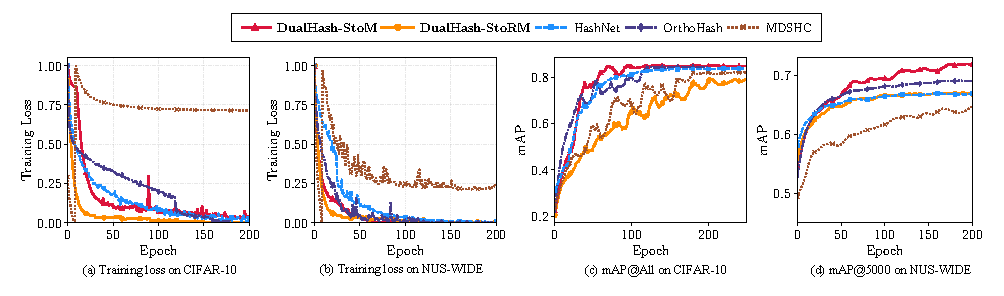
\includegraphics[width=0.95\linewidth]{results_images/ex1_4figures_new.pdf}
    \caption{Training loss and the mAP results of DualHash and baselines with 64 bits on CIFAR-10 and NUS-WIDE datasets.}
    \label{fig:training_loss_map_2datasets}
    \vspace{-2ex}
\end{figure}
\begin{figure}[t]
    % \vspace{-1mm}
    \centering
    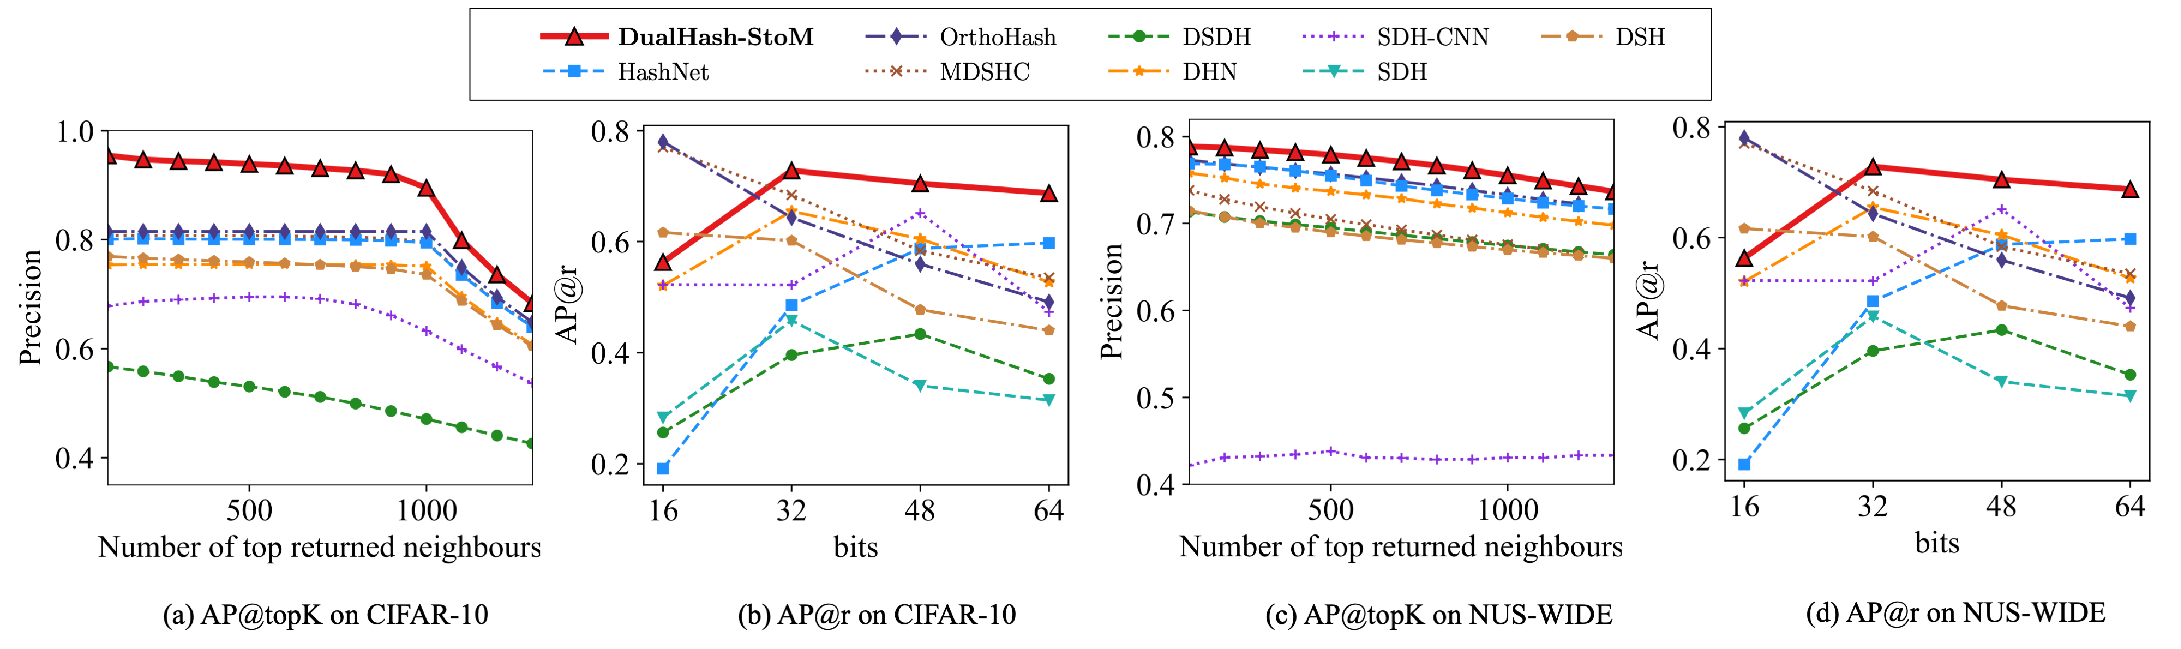
\includegraphics[width=0.95\linewidth]{results_images/ex2_4figures.pdf}
    \caption{Retrieval performance of DualHash and baselines on CIFAR-10 and NUS-WIDE datasets. (a), (c): P@topK with 64 bits;  (b), (d): P@r(=2) with different numbers of bits.}
 \label{fig:retrieval_2datasets}
    \vspace{-2ex}
\end{figure}
\begin{table}[t]
    \centering
    \caption{The mAP results of DualHash and baselines with different numbers of bits on CIFAR-10 and NUS-WIDE datasets with ResNet50 backbone.}
    \label{Table: performance_comparison_resnet50_small}
    \resizebox{\linewidth}{!}{
    \begin{tabular}{ccccccccc}
        \toprule
         & \multicolumn{4}{c}{CIFAR-10 (mAP@All)} & \multicolumn{4}{c}{NUS-WIDE (mAP@5000)} \\
        \cmidrule(lr){2-5} \cmidrule(lr){6-9}
         Method (ResNet50) & 16 bits & 32 bits & 48 bits & 64 bits & 16 bits & 32 bits & 48 bits & 64 bits \\
        \midrule
        DSH \cite{liuDeepSupervisedHashing} & 0.7403 & 0.8116 & 0.8217 & 0.8239 & 0.5559 & 0.6952 & 0.6981 & 0.7165 \\
        OrthoHash \cite{hoeOneLossAll2021} & \textbf{0.9032} & 0.9182 & 0.9202 & 0.9224 & \textbf{0.7448} & 0.7600 & 0.7569 & 0.7863 \\
        MDSHC \cite{wang2023deep} & 0.8980 & 0.9007 & 0.9063 & 0.9227 & 0.6428 & 0.7002 & 0.7248 & 0.7758 \\
        \cmidrule(lr){2-9}
        DualHash-StoM & 0.8559 & \textbf{0.9202} & \textbf{0.9392} & \textbf{0.9416} & 0.6538 & \textbf{0.7783} & \textbf{0.7721} & \textbf{0.8016} \\
        \bottomrule
    \end{tabular}}
    \vspace{2ex}
    \parbox{\linewidth}{\footnotesize
    \textbf{Bold} values indicate the best results.
    }
    \vspace{-1ex}
\end{table}
We provide empirical evidence that is consistent with our theoretical results (Theorems \ref{Theorem: the oracle complexity in SGDM} and \ref{Theorem: the oracle complexity in STORM}) and compare with HashNet, OrthoHash, and MDSHC with 64 bits on CIFAR-10 and NUS-WIDE. 
\Cref{fig:training_loss_map_2datasets} shows the training loss and validation mAP curves over epochs.
As shown in \Cref{fig:training_loss_map_2datasets} (a)-(b), DualHash-StoRM achieves the fastest convergence and lowest loss values on CIFAR-10 and NUS-WIDE, requiring only approximately 25 epochs on CIFAR-10. This aligns with our theoretical outcome: the variance reduction mechanism accelerates convergence. Though slower than DualHash-StoRM, DualHash-StoM still outperforms other baselines (approximately 75 epochs on CIFAR-10). 
Meanwhile, \Cref{fig:training_loss_map_2datasets} (c)-(d) show that although DualHash-StoRM converges faster during training, DualHash-StoM ultimately exhibits superior retrieval performance compared to other baselines. 
% \vspace{3pt}
\subsection{Comparison of Retrieval Performance}
\label{Subsection: Comparison of retrieval performance}
\begin{table}[t]
% \vspace{2ex}
    \centering
    \caption{The mAP results of DualHash and baselines with different numbers of bits on the ImageNet-100 dataset with ResNet50 backbone.}
    \label{tab:performance_imagenet_resnet50}
    \small
    \begin{tabular}{lcccc}
     \toprule
 & \multicolumn{4}{c}{ImageNet-100 (mAP@1000)} \\
\cmidrule(lr){2-5}
Method (ResNet50) & 16 bits & 32 bits & 48 bits & 64 bits \\
\midrule
DSH \cite{liuDeepSupervisedHashing} & 0.7179 & 0.7448 & 0.7335 & 0.7585 \\
OrthoHash \cite{hoeOneLossAll2021} & 0.8040 & \textbf{0.8292} & 0.8510 & 0.8636 \\
MDSHC \cite{wang2023deep} & \textbf{0.8047} & 0.8131 & 0.8561 & 0.8657 \\
 \cmidrule(lr){2-5}
DualHash-StoM & 0.7402 & 0.7705 & \textbf{0.8662} & \textbf{0.8714} \\
        \bottomrule
    \end{tabular}
    \vspace{2ex}
    \parbox{\linewidth}{\footnotesize
    \textbf{Bold} values indicate the best results.
    }
    \vspace{-2ex}
\end{table}
We report retrieval performance on CIFAR-10 and NUS-WIDE datasets, as shown in Table \ref{Table: baselines mAP}
% , \ref{Table: performance_comparison_resnet50_small}, \ref{tab:performance_imagenet_resnet50} 
and \Cref{fig:retrieval_2datasets}. 
In terms of mAP, DualHash methods consistently outperform most baselines, including recent advanced methods like OrthoHash and MDSHC.
On CIFAR-10, DualHash-StoM achieves 0.8539 mAP with 64 bits, outperforming OrthoHash (0.8355). On the NUS-WIDE dataset, it reaches 0.7448 mAP, significantly superior to MDSHC (0.6493).  
Although slightly less accurate than the StoM variant, DualHash-StoRM remains comparable to other baselines, providing a trade-off between accuracy and efficiency. 

To further demonstrate the scalability of our approach, we evaluate our method and three baselines using a \textbf{ResNet50 backbone}. As shown in \Cref{Table: performance_comparison_resnet50_small}, this modern architecture brings substantial performance gains in terms of mAP for all methods across CIFAR-10 and NUS-WIDE. Our DualHash-StoM, for example, achieves mAP improvements of 10.3\% on CIFAR-10 (0.9416 vs 0.8539) and 7.6\% on NUS-WIDE (0.8016 vs 0.7448) at 64 bits. Nevertheless, our method consistently maintains peak performance at 32 bits or more, outperforming all baseline methods. Moreover, on the more complex ImageNet-100 dataset, our method continues to demonstrate superior performance. As reported in \Cref{tab:performance_imagenet_resnet50}, DualHash-StoM reaches 86.62\% and 87.14\% mAP at 48 and 64 bits, outperforming all baselines. These results confirm that our method maintains robust performance and strong generalization capability as data complexity increases.

For P@topK (\Cref{fig:retrieval_2datasets} (a),(c)),  DualHash maintains 0.9 precision at lower top-k values on CIFAR-10, significantly outperforming other methods. This indicates that our method is suitable for precision-oriented image retrieval systems.
For P@r=2 (\Cref{fig:retrieval_2datasets} (b),(d)), DualHash-StoM consistently maintains peak performance at 32 bits and above, with 32 bits being optimal across CIFAR-10 and NUS-WIDE. These results align with the fact that as bit length increases, the Hamming space becomes sparse and few data points fall within the Hamming ball with radius 2 \cite{norouzi2012fast}.
% \vspace{3pt}

\subsection{Quantization Error Analysis}
\label{Subsection: Further analysis}
\begin{figure}[t]
% \vspace{-2ex}
    \centering
    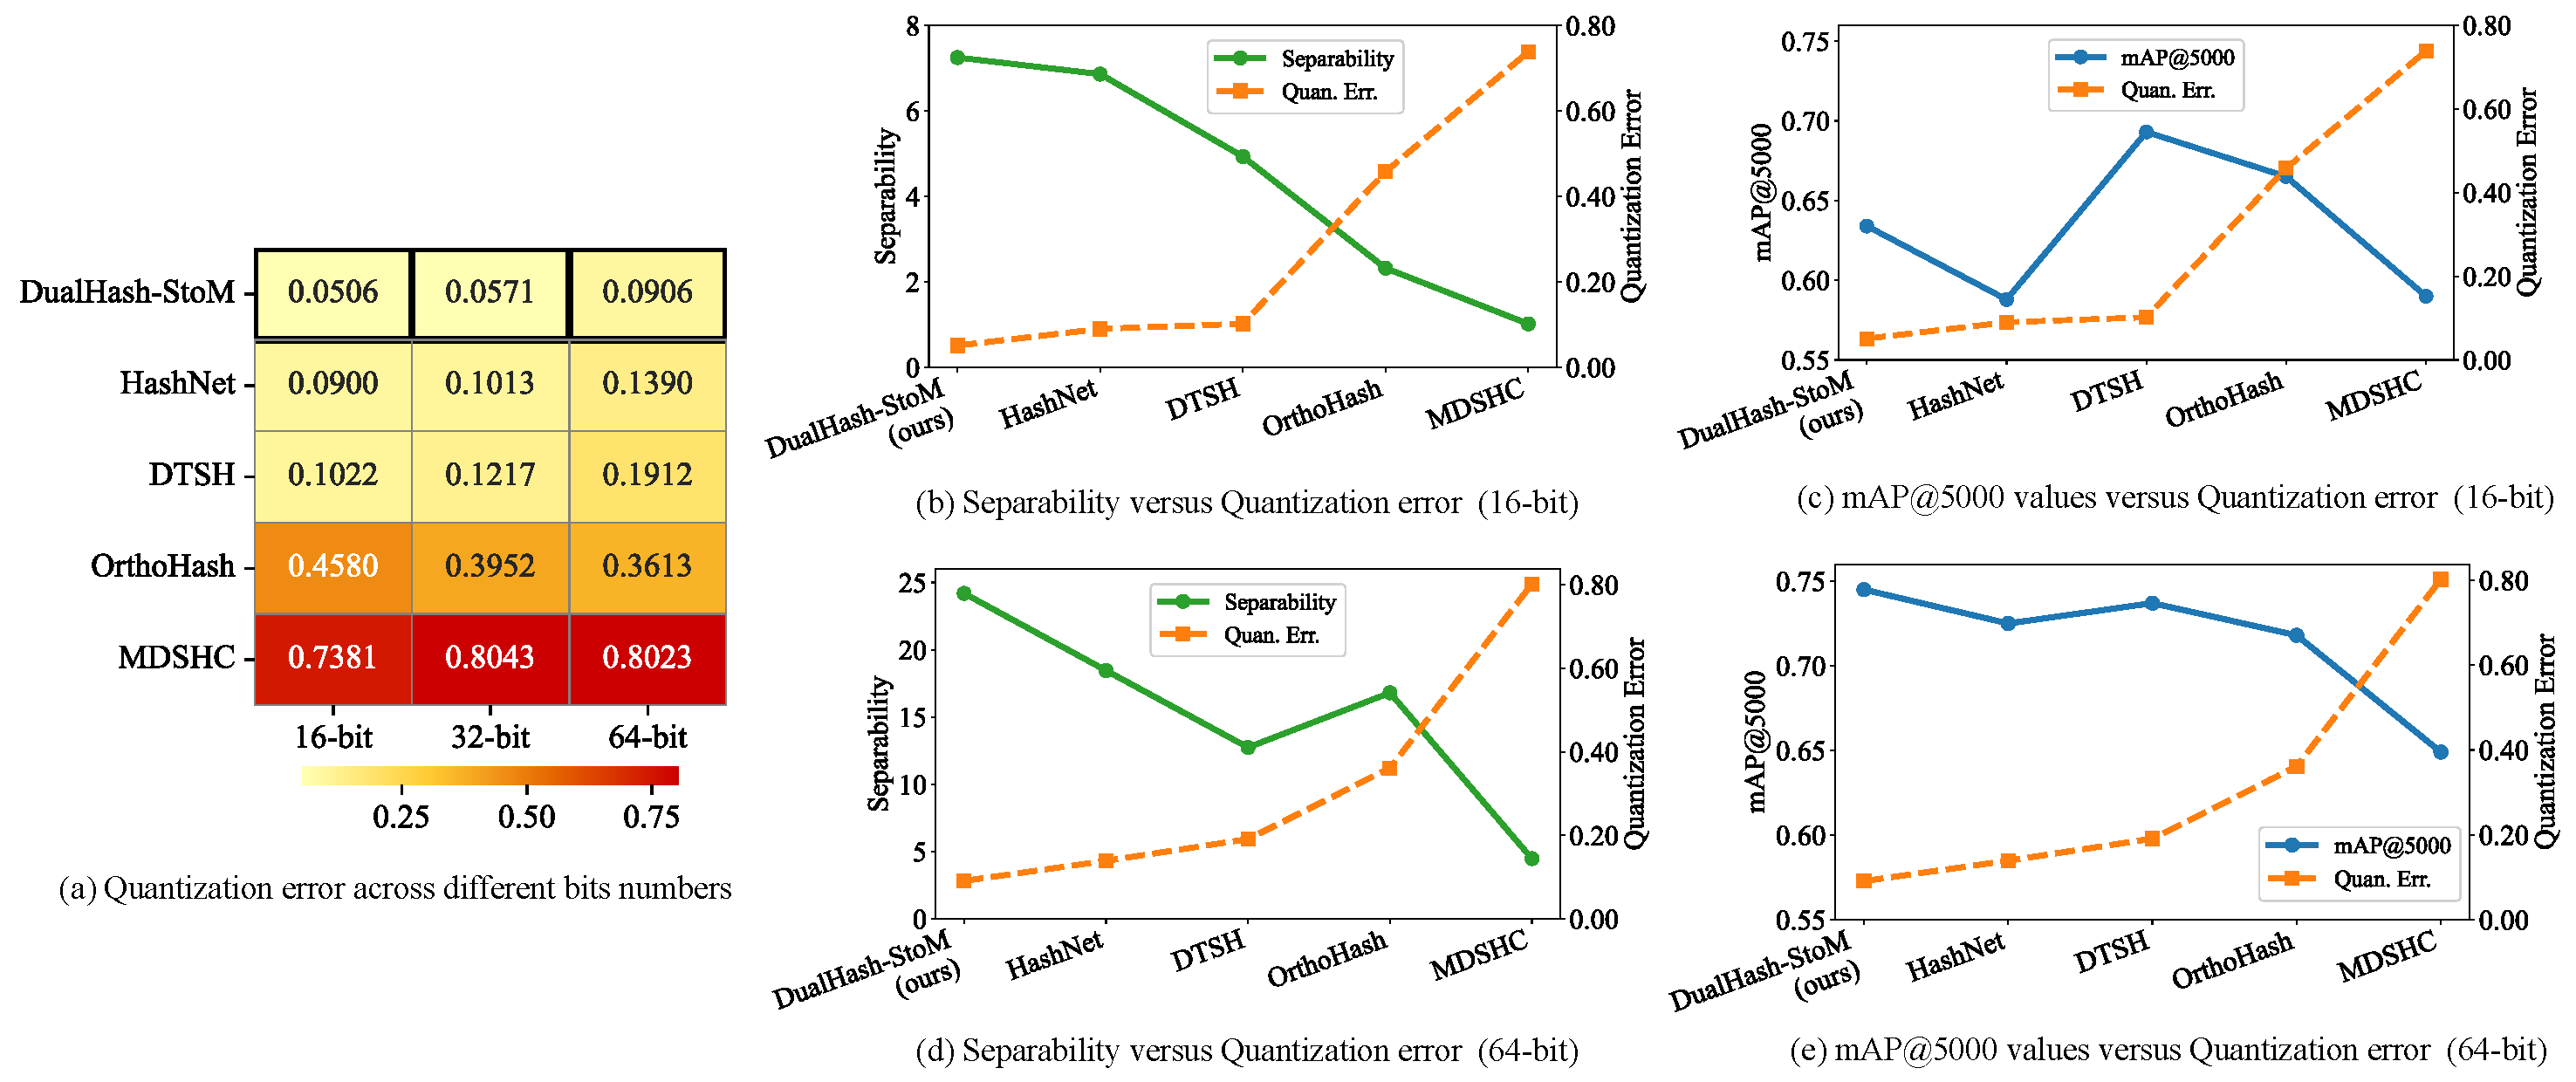
\includegraphics[width=0.95\linewidth]{results_images/quantization_error_further_analysis.pdf}
    \caption{Quantization error and its impact on retrieval performance across different numbers of bits on  NUS-WIDE.}
    \label{fig:quantization_error}
\end{figure}
\begin{figure}[t]
    \vspace{-2ex}
    \centering
    \includegraphics[width=0.95\linewidth]{results_images/hamming_hig_64.pdf}
    \caption{Histogram of intra-class and inter-class Hamming distances of DualHash and baselines with 64 bits on the NUS-WIDE dataset. The arrow annotation is the separability in Hamming distances, \(\EE [D_{inter}] - \EE [D_{intra}]\). We normalized the frequency so that the sum of all bins equals to 1.}
    \label{fig: His_64_NUSWIDE}
    \vspace{-2ex}
\end{figure}
\begin{figure}[t]
    \vspace{-2ex}
    \centering
    \includegraphics[width=0.95\linewidth]{results_images/hamming_hig_16.pdf}
    \caption{Histogram of intra-class and inter-class Hamming distances of DualHash and baselines with 16 bits on NUS-WIDE.}
    \label{fig: His_16_NUSWIDE}
    \vspace{-2ex}
\end{figure}
\begin{figure}[t]
    % \vspace{-1mm}
    \centering
    \includegraphics[width=0.95\linewidth]{results_images/sensitivity_2datasets.pdf}
    \caption{The mAP results of DualHash-StoM with Different settings of \(\eta\) and \(\lambda\) with 64 \& 16 bits on CIFAR-10 and NUS-WIDE.}
    \label{fig: sensitivity analysis of DualHash}
    \vspace{-2ex}
\end{figure}
To elucidate the mechanisms behind the performance of DualHash, following \cite{hoeOneLossAll2021},
we examine the quantization error (the discrepancy between continuous outputs and binary codes, \Cref{fig:quantization_error}) and the Hamming distance distributions of the resulting hash codes (\Cref{fig: His_64_NUSWIDE,fig: His_16_NUSWIDE}) across different bit lengths $K$ on the NUS-WIDE dataset. We compare DualHash-StoM against four deep hashing methods: HashNet \cite{Cao2017HashNetDL} and OrthoHash \cite{hoeOneLossAll2021} (employing distinct quantization strategies), and DTSH \cite{wang2016DTSH} and MDSHC \cite{wang2023deep} (both utilizing $W$-type regularization).

\vspace{3pt}
\noindent\textbf{Quantization Error Correlates with Intra- and Inter-class Distances.}
We find that methods achieving smaller quantization errors produce hash codes with reduced intra-class distances and enhanced inter-class separability, as shown in \Cref{fig:quantization_error}(a) and \Cref{fig: His_16_NUSWIDE,fig: His_64_NUSWIDE}. In the 64-bit setting (\Cref{fig: His_64_NUSWIDE}), both HashNet and DualHash exhibit similar inter-class distributions (close to Hamming distance $K/2 = 32$). However, DualHash's lower quantization error (0.0906 vs. 0.1390) enables significantly superior separability, i.e., the difference in the mean of intra-class distance (the blue dotted line)
with the mean of inter-class distance (the orange dotted line). In contrast, MDSHC's high quantization error (0.8023) leads to substantially larger intra-class distances and weaker inter-class separation, yielding a $5\times$ inferior separability ratio (24.19 vs. 4.47). 
This demonstrates that reducing quantization error enhances code quality primarily by compressing intra-class distributions.

\vspace{3pt}
\noindent\textbf{DualHash Achieves Lower Quantization Error via Dual-Space Reformulation.}
As shown in \Cref{fig:quantization_error}(a), DualHash attains the smallest quantization error across different bit lengths among all evaluated methods. This performance advantage stems from a fundamental methodological innovation: DualHash employs a novel dual-space reformulation of the W-regularization. The convexity property inherent in our dual formulation's conjugate function yields significant optimization advantages compared to directly optimizing the original nonconvex regularization or activation functions. 

\vspace{3pt}
\noindent\textbf{Bit-Dependent Performance and the Separability-Semantics Trade-off.}
While lower quantization error generally improves separability (\Cref{fig:quantization_error}(b) and (d)), its impact on retrieval performance varies significantly across bit settings, revealing a fundamental trade-off between class separability and semantic preservation.

\noindent\textit{High-bit regime ($K = 64$): Lower quantization error helps produce high mAP.}
At $K = 64$ (Figures \ref{fig:quantization_error}(d) and (e)), lower quantization error consistently correlates with higher mAP by enhancing separability and preserving both semantic discriminability and visual feature quality. Methods achieving low quantization loss (e.g., DualHash, HashNet, and DTSH) demonstrate superior retrieval accuracy, with DualHash achieving peak mAP performance.

\noindent\textit{Low-bit regime ($K = 16$): Low quantization error may produce low performance.}
At $K = 16$ (\Cref{fig:quantization_error}(b) and (c)), we observe a contrasting pattern: both extremely low and extremely high quantization error methods yield suboptimal performance. Notably, DTSH, which maintains intermediate quantization error, achieves superior mAP. Methods with very low quantization error (e.g., DualHash and HashNet) exhibit relatively lower mAP, particularly on multi-label datasets (e.g., NUS-WIDE). Specifically, we observe that  DualHash generates hash codes with low intra-class distances and high inter-class separation. This creates relatively clean class separation, but the actual visual relationships between images may get lost. Consequently, DualHash excels on simple datasets like CIFAR-10 but shows relatively lower performance on complex datasets like NUS-WIDE (multi-label) and ImageNet-100 (large-scale single-label).

% \vspace{3pt}
\subsection{Parameter Sensitivity Analysis}
To explore the sensitivity of key hyperparameters $\eta$ and $\lambda$ in 
DualHash, we conduct a grid search with $\eta \in \{10^{-4}, 10^{-3}, 
10^{-2}, 10^{-1}\}$ and $\lambda \in \{10^{-3}, 10^{-2}, 5\times 10^{-2}, 10^{-1}\}$. Unlike many deep hashing 
methods that exhibit significant hyperparameter sensitivity, DualHash-StoM 
demonstrates robust performance across a wide range of hyperparameter 
combinations (see \Cref{fig: sensitivity analysis of DualHash}). 
Specifically, 64-bit codes achieve excellent stability with mAP variations 
below 3\% on CIFAR-10 and 8\% on NUS-WIDE. While 16-bit codes show greater 
sensitivity (up to 18\% on CIFAR-10), this behavior is consistent with the 
intrinsic optimization challenges of extremely compact hash codes. Overall, 
the method demonstrates strong stability for standard hash lengths ($\geq$64 bits), 
which simplifies hyperparameter tuning in practical high-precision retrieval 
applications.

\section{Conclusion and Discussion}
\label{Section: Conclusion}
This paper proposed DualHash, a stochastic primal-dual algorithm for deep hashing with rigorous non-asymptotic convergence guarantees. Our approach effectively addressed the fundamental optimization challenge of W-type regularization with nonlinear composition through a novel ``decoupling-dual-structure'' strategy: transforming the nonconvex regularizer into a convex dual space with closed-form proximal updates. We provided a distinct theoretical framework beyond conventional primal-dual analysis, establishing complexity bounds of $\mathcal{O}(\varepsilon^{-4})$ for DualHash-StoM and optimal $\mathcal{O}(\varepsilon^{-3})$ for DualHash-StoRM. Extensive experiments validated  DualHash achieved superior retrieval performance across all metrics, including the highest mAP at 32 bits or more, consistently lower quantization errors, and stronger robustness on both datasets. 

Beyond deep hashing, our core \textbf{decoupling-dual-structure} optimization principle offered a promising pathway for tackling nonconvex regularization challenges in related domains, including neural network quantization \cite{BinaryConnect,Bai2018ProxQuantQN,Yang2019QuantizationN} and sparse regularized neural network training \cite{bui2021structured,louizos2018learning,xu2012l,wen2016learning}.

% \section{References Section}
\bibliographystyle{IEEEtran}
\bibliography{refers}

\clearpage
\section*{Supplementary Material A}
% % !TEX root = main.tex
% \documentclass[journal]{IEEEtran}
% \input{tip_shared}
% \allowdisplaybreaks[2]

% % 跨文档引用配置
% \usepackage{xr-hyper}  % 推荐使用 xr-hyper（支持hyperref）
% \usepackage{hyperref}  % 如果需要超链接支持

% \externaldocument{main}  

This supplementary material provides detailed experimental settings and additional results.

% In \Cref{Appendix: Preliminaries and notations}, we give some basic definitions and lemmas for the following analysis.

% In \Cref{Appendix: main proofs}, we discuss the main assumptions.

% In \Cref{Appendix: Experiment details}, we provide the experimental details and additional experiments.

\section{Experiments details}
\label{Appendix: Experiment details} 
\subsection{Deep Pairwise Supervised Hashing Formulation}
\label{Appendix: hashing formulation}

We consider deep supervised pairwise hashing in our experiments, which aims to learn binary codes that minimize Hamming distances for similar pairs and maximize them for dissimilar pairs. Let $\bA = \{\ba_i \in \RR^{d_a} : i = 1, \ldots, n\}$ be the training set with labels $\calY = \{\by_i \in \{0,1\}^C\}$ (one-hot for single-label, multi-hot for multi-label). Key notations are in \Cref{Table:notations_for_deep_hashing}.


\paragraph{Network Architecture}  
A CNN extracts features from $\ba_i$, followed by a fully connected hash layer producing $d$-dimensional outputs $\bC(\bx; \ba_i)$, which are passed through $\tanh$ to yield $\bu_i$.


\paragraph{Loss Function}  
For hash codes in $\{-1,1\}^d$, the Hamming distance is $d_{ij}^h = \tfrac{1}{2}(d - \langle \bh_i, \bh_j \rangle)$. Following \cite{xiaSupervisedHashingImage2014,laiSimultaneousFeatureLearning2015}, similarity $s^o_{ij} = 1$ if samples share labels, else $0$. The likelihood is:
\[
P(s^o_{ij} \mid \bh_i, \bh_j) = \sigma(\langle \bh_i, \bh_j \rangle)^{s^o_{ij}} \left(1 - \sigma(\langle \bh_i, \bh_j \rangle)\right)^{1 - s^o_{ij}},
\]
where $\sigma(x) = (1 + \exp(-\alpha x))^{-1}$, $\alpha < 1$. Using continuous codes $\bu_i$ and $s^h_{ij} = \tfrac{1}{2} \langle \bu_i, \bu_j \rangle$, the loss becomes:
\begin{align}
\label{Eq: the pairwise CE loss}
\min_{\bx} \; \calL_S(\bx) = -\frac{1}{|\calS|} \sum_{s^o_{ij} \in \calS} \log\left(1 + \exp\left(-\alpha s^o_{ij} s^h_{ij}\right)\right).
\end{align}

We use the W-type regularization:
\begin{align}
\label{Eq: the W-type regularization}
h(\bZ) = \sum_{i=1}^n h(\bz_i), \quad h(\bz) = \lambda \|\,|\bz| - \bm{1}\,\|_1,
\end{align}
where $\lambda > 0$ controls regularization strength.

Combining \eqref{Eq: the pairwise CE loss} and \eqref{Eq: the W-type regularization} into \eqref{Prop: block-wise regularized problem} gives the final loss of DualHash in our experiments.
\begin{align}
% \label{Eq: the pairwise quantization-based hashing}
\min_{\bx \in \calX, \bB \in \calB} \; 
&-\frac{1}{|\calS|} \sum_{s^o_{ij} \in \calS} \log\left(1 + \exp\left(-\alpha s^o_{ij} s^h_{ij}\right)\right) \notag \\
&+ \frac{\gamma}{2n}\sum_{i=1}^n \| \bb_i - \bu_i\|_2^2 
+ \sum_{i=1}^n \lambda \|\,|\bb_i| - \bm{1}\,\|_1. \notag
\end{align}


\paragraph{Out-of-sample Extension}  
For an unseen query $\ba_q \notin \bA$, its binary code is predicted as:
\[
\bb_q = \operatorname{sgn}(\bC(\bx; \ba_q)).
\]
\begin{table}[t]
    \centering
    \caption{Summary of symbols and notations.}
    \label{Table:notations_for_deep_hashing}
    \small
    \begin{tabular}{ll}
        \toprule 
        \textbf{Symbol} & \textbf{Description} \\
        \midrule 
        $\ba_{i}$, $\by_{i}$ & Input feature and label vector for \\
                             & $i$-th sample \\
        $s_{ij}^{o}$, $s_{ij}^{h}$ & Similarity in input space and \\
                                   & Hamming space \\
        $d_{ij}^{o}$, $d_{ij}^{h}$ & Distance in input space and \\
                                   & Hamming space \\
        $\bC(\bx; \ba_{i})$ & Network output before activation \\
        $\bb_{i}\in \{-1, 1\}^{d}$ & Binary hash code for $i$-th sample \\
        $\bu_{i}= \tanh(\bC(\bx; \ba_{i}))$ & Continuous code after activation \\
        $n$, $d$ & Number of samples and hash \\
                 & code length \\
        $\bx$ & Network parameters \\
        $d_{\ba}$, $d_{x}$ & Dimension of input feature and \\
                           & parameters \\
        \bottomrule
    \end{tabular}
\end{table}

\subsection{Details of experiment implementation}
\label{Appendix: Details of experiment implementation}
\paragraph{Baseline methods}
We compare our method with eight baseline approaches, including one traditional discrete hashing method and seven deep supervised hashing methods:
\begin{enumerate}[label=(\roman{*}),leftmargin=2em]
    \item \textbf{SDH}~\cite{shenSupervisedDiscreteHashing2015}: A pointwise supervised hashing method using hand-crafted features. It employs discrete cyclic coordinate descent to directly optimize binary codes.
    
    \item \textbf{DHN}~\cite{zhuDeepHashingNetwork2016}: A Bayesian framework that minimizes pairwise cross-entropy loss and quantization error using $\tanh$ relaxation and $\sum_i\log(\cosh(|z_i|-1))$ regularization.
    
    \item \textbf{DSH}~\cite{liuDeepSupervisedHashing}: Uses max-min pairwise loss with $\||\bz|-\bm{1}\|_1$ regularization to minimize quantization error.
    
    \item \textbf{DTSH}~\cite{wang2016DTSH}: Learns hash codes by maximizing triplet likelihood with negative log-triplet loss, using  $\||\bz|-\bm{1}\|^2_2$  quantization regularization and a positive margin $\alpha$ to accelerate training and normalize Hamming distance gaps.
    
    \item \textbf{HashNet}~\cite{Cao2017HashNetDL}: Progressively increases $\beta$ in $\tanh(\beta x)$ to approximate the $\text{sgn}$ function, addressing nonconvex optimization challenges.
    
    \item \textbf{DSDH}~\cite{li2017deep}: Integrates pairwise labels and classification information using alternating minimization to learn features and binary codes with the $\text{sgn}$ function.
    
    \item \textbf{OrthoHash}~\cite{hoeOneLossAll2021}: Uses a single cosine similarity loss to maximize alignment between continuous codes and binary orthogonal codes, ensuring discriminativeness with minimal quantization error.
    
    \item \textbf{MDSHC}~\cite{wang2023deep}: A two-stage method that first generates hash centers with minimal Hamming distance constraints, then uses three-part losses with $\||\bz|-\bm{1}\|_1$ regularization to reduce quantization error.
\end{enumerate}


\paragraph{Evaluation Protocols}
Following \cite{liuDeepSupervisedHashing}, we adopt three evaluation metrics:

\begin{enumerate}[label=\textup{(\roman{*})}, leftmargin=2em]
    \item \textit{Mean Average Precision (mAP)}: For a query $\bx_q$, the Average Precision is computed as:
    \[
        \text{AP}(\bx_q) = \frac{\sum_{k=1}^{N} P(k) \cdot \mathbb{I}_{\text{rel}}(k)}{\min(N, R_q)},
    \]
    where $P(k)$ is precision at rank $k$, $\mathbb{I}_{\text{rel}}(k)$ indicates whether the $k$-th result is relevant, $R_q$ is the total relevant samples, and $N$ is the number of retrieved items. mAP averages AP over all queries. For CIFAR-10, we use all returned neighbors; for NUS-WIDE, we consider top-5000 results.
    
    \item \textit{Precision at Top K (AP@topK)}: The proportion of true neighbors among top-K retrieved results, averaged over all queries.
    
    \item \textit{Precision within Hamming Radius 2 (AP@r)}: Measures retrieval accuracy for items within Hamming distance 2 from the query. This metric is particularly efficient as Hamming radius search has $\mathcal{O}(1)$ time complexity per query.
    
    \item \textit{Precision-recall curves of Hamming ranking}: PR curves illustrate
        precision at various levels of recall, offering insights into the trade-off between precision and recall at different thresholds. These curves are widely
        recognized as effective indicators of the robustness and overall performance
        of different algorithms.
\end{enumerate}

\section{Additional Experiments Results}
\subsection{Comparison of Optimization Algorithms with Different W-Type Regularizations}
\begin{table*}[!t]
    \centering
    \caption{Configurations of different W-type regularizations and optimization algorithms \\ for DualHash-StoM and three baselines.}
    \label{tab:4_algorithms_for_hash_regularization_and_update}
    \resizebox{0.93\textwidth}{!}{
    \begin{tabular*}{1\textwidth}{@{\extracolsep{\fill}}lcccc@{}}
        \toprule 
        Method & $h(\bz)$ & Convexity & Algorithm & Complexity \\
        \midrule 
        DSH \cite{liuDeepSupervisedHashing} & $\| |\bz| - \mathbf{1}\|_{1}$ & Nonconvex & SGDM & -- \\
        StoMHash-WCR & $\| \bz^{2}- \mathbf{1}\|_{1}$ & Weakly convex & SPGD & -- \\
        DHN \cite{zhuDeepHashingNetwork2016} & $\sum_{i}\log(\cosh(|z_{i}| - 1))$ & Nonconvex & SGDM & -- \\
        \textbf{DualHash-StoM} & $\| |\bz| - \mathbf{1}\|_{1}$ & Nonconvex & PD & $\checkmark$ \\
        \bottomrule
    \end{tabular*}}
    \vspace{-3pt}
    \parbox{0.93\textwidth}{\footnotesize
    \textbf{Notes}: \textbf{Algorithm} describes the optimization strategy: SGDM (stochastic subgradient descent with momentum), SPGD (stochastic proximal gradient descent), PD (primal-dual). \textbf{Complexity} reports oracle complexity; `--' indicates no analysis available.
    }
\end{table*}
To validate the effectiveness of our primal-dual framework, we compare DualHash-StoM
against optimization algorithms with different W-type regularizations. \Cref{tab:4_algorithms_for_hash_regularization_and_update}
summarizes the configurations of different regularization functions and their corresponding optimization approaches. For StoMHash-WCR, we employ the regularization $\lambda \| \bz^{2}- \mathbf{1}\|_1$
following the iSPALM framework \cite{InertialProximalAlternating}. The proximal
operator is computed with parameter $\rho > 0$ under the condition
$\frac{\rho}{\eta}> \frac{1}{2}$, which ensures the subproblem is strongly convex
with a unique solution.
% $$\text{prox}_{\rho f}(\bx) = \arg \min_{y}\left( \eta \|\by^{2}- \mathbf{1}\| + \frac{\rho}{2} \|\by - \bx\|^{2}\right).$$
\begin{figure*}[htbp]
    \centering
    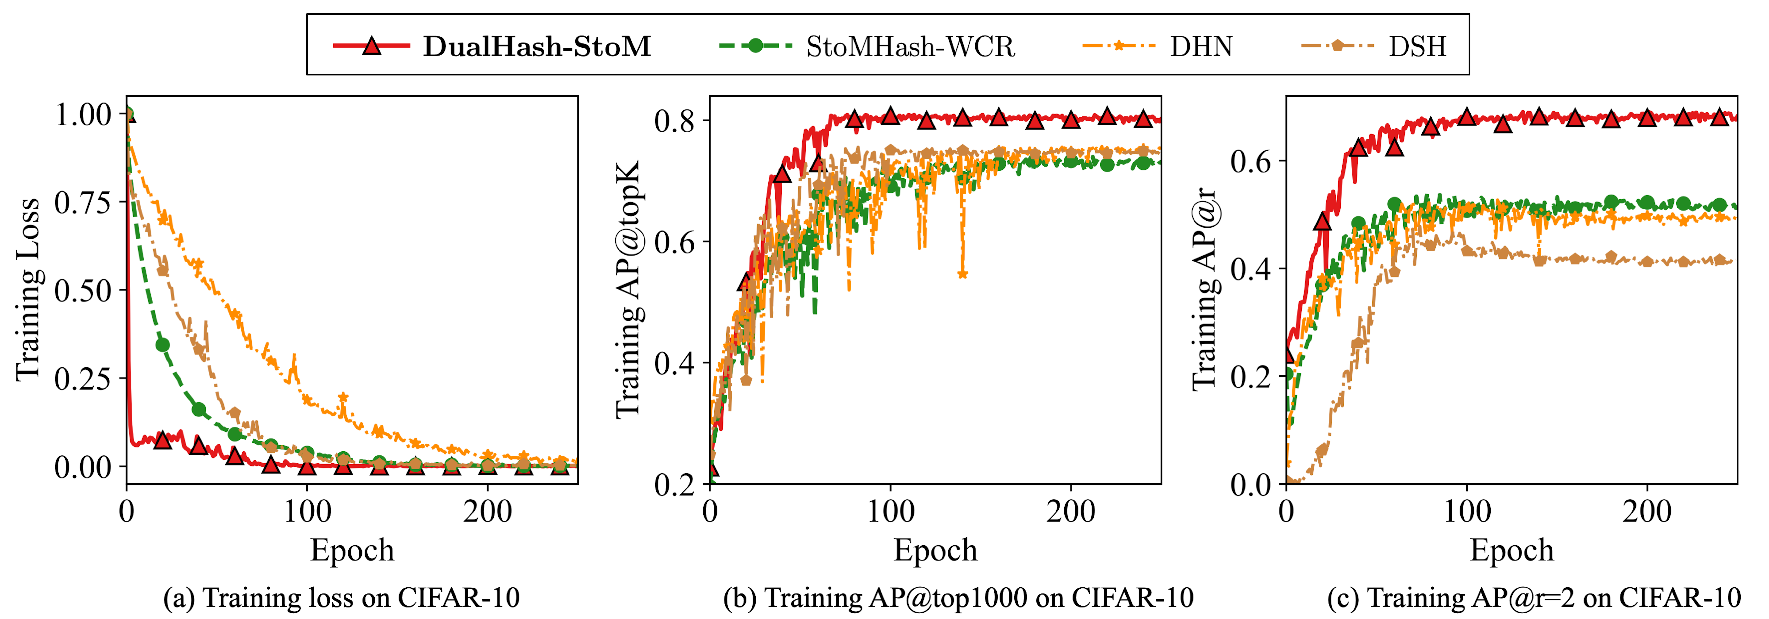
\includegraphics[width=0.8\textwidth]{results_images/ex3_training_cifar10.pdf}
    \caption{Training performance comparison of DualHash-StoM and three baselines with 64 bits on the CIFAR-10 dataset.}
    \label{Fig: Comparison of training performance of Different Methods on CIFAR-10}
\end{figure*}
\begin{figure*}[htbp]
    \centering
    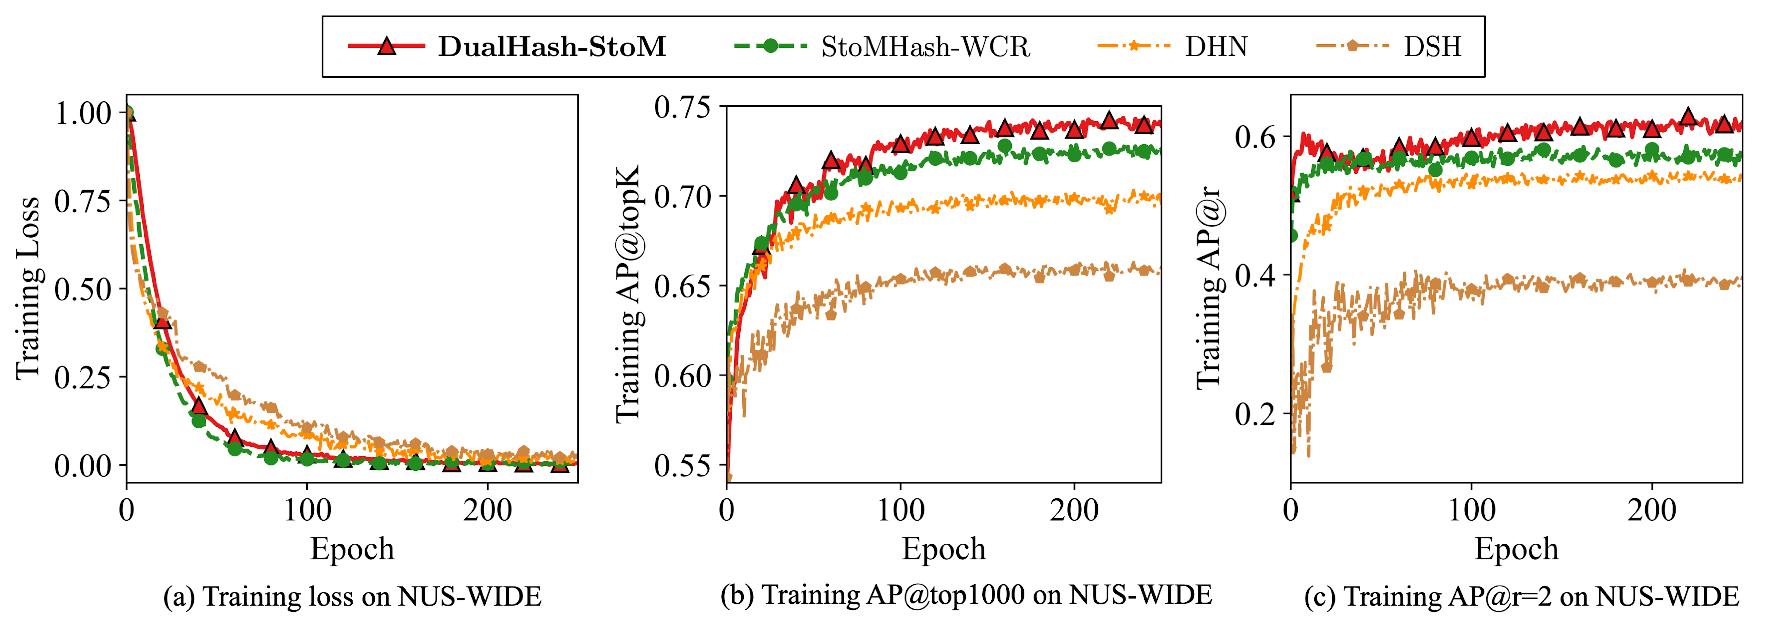
\includegraphics[width=0.8\textwidth]{results_images/ex3_training_nuswide.pdf}
    \caption{Training performance comparison of DualHash-StoM and three baselines with 64 bits on the NUS-WIDE dataset.}
    \label{Fig: Comparison of training performance of Different Methods on NUS-WIDE}
\end{figure*}


\paragraph{Training performance analysis}
\begin{table*}[htbp]
    \centering
    \caption{Retrieval performance comparison of DualHash-StoM and three baselines with 64 bits \\ on CIFAR-10 and NUS-WIDE datasets}
    \label{tab:performance_comparison_64bits}
    \resizebox{0.93\textwidth}{!}{
    \begin{tabular*}{1\textwidth}{@{\extracolsep{\fill}}lcccccc@{}}
        \toprule 
        \multirow{2}{*}{Methods} & \multicolumn{3}{c}{CIFAR-10} & \multicolumn{3}{c}{NUS-WIDE} \\
        \cmidrule(lr){2-4} \cmidrule(lr){5-7}
         & mAP@All & AP@r & Time\textsuperscript{*} & mAP@5000 & AP@r & Time\textsuperscript{*} \\
        \midrule 
        DSH \cite{liuDeepSupervisedHashing} & 0.8010 & 0.4401 & 7.38 & 0.6634 & 0.4004 & 21.14 \\
        DHN \cite{zhuDeepHashingNetwork2016} & \textcolor{blue}{0.8051} & 0.5272 & \textcolor{red}{\textbf{6.74}} & 0.7042 & 0.5432 & \textcolor{red}{\textbf{16.47}} \\
        StoMHash-WCR & 0.7773 & \textcolor{blue}{0.5402} & 7.04 & \textcolor{blue}{0.7225} & \textcolor{blue}{0.5857} & \textcolor{blue}{16.69} \\
        \textbf{DualHash-StoM} & \textcolor{red}{\textbf{0.8539}} & \textcolor{red}{\textbf{0.6872}} & \textcolor{blue}{6.86} & \textcolor{red}{\textbf{0.7448}} & \textcolor{red}{\textbf{0.6548}} & 16.83 \\
        \bottomrule
    \end{tabular*}}
    
    \parbox{0.93\textwidth}{\footnotesize
    \textsuperscript{*}Training time per epoch (seconds). \textbf{\textcolor{red}{Red}} and \textcolor{blue}{blue} indicate highest and second highest values.
    }
\end{table*}
Figures \ref{Fig: Comparison of training performance of Different Methods on CIFAR-10} and \ref{Fig: Comparison of training performance of Different Methods on NUS-WIDE} present
training dynamics across different optimization approaches, comparing training loss, AP@top1000, and AP@r=2 metrics \textbf{with 64 bits} on both datasets. On
CIFAR-10, DualHash-StoM demonstrates superior optimization efficiency across all
metrics. Our method achieves the fastest convergence in training loss while consistently maintaining the highest AP@r and AP@top1000 values throughout the
optimization process. While StoMHash with weakly convex regularization (StoMHash-WCR)
shows competitive performance, DualHash-StoM achieves both faster convergence
and consistently higher performance, demonstrating the effectiveness of our
primal-dual transformation for handling W-type regularizations. On the more challenging NUS-WIDE dataset with complex multi-label scenarios, DualHash-StoM maintains
competitive retrieval performance despite slightly slower initial convergence.
The experimental results on diverse datasets confirm our core motivation:
utilizing nonconvex nonsmooth regularization with specialized primal-dual
optimization significantly improves hash code learning and retrieval
performance in practical applications.

\paragraph{Retrieval performance in hamming space}
We report mAP, AP@r, and the average time per training epoch on both datasets, all
with 64-bit codes, for different methods in
Table~\ref{tab:performance_comparison_64bits}. The results highlight the superior retrieval
accuracy of DualHash-StoM compared to the baseline methods.

Specifically, on the CIFAR-10 dataset, DualHash-StoM achieves 9.9\% and 27.2\%
improvements over StoMHash-WCR in mAP@All and AP@r, respectively. Similarly, on the
NUS-WIDE dataset, DualHash-StoM outperforms StoMHash-WCR with a 3.1\% improvement
in mAP@5000 and an 11.8\% improvement in AP@r. Computationally, DualHash-StoM shows comparable efficiency to baselines such as DHN
(e.g., 6.86s vs. 6.74s on CIFAR-10 and 16.83s vs. 16.47s
on NUS-WIDE). This marginal time increase is justified by the substantial performance gains.
\begin{figure*}[!t]
    \centering
    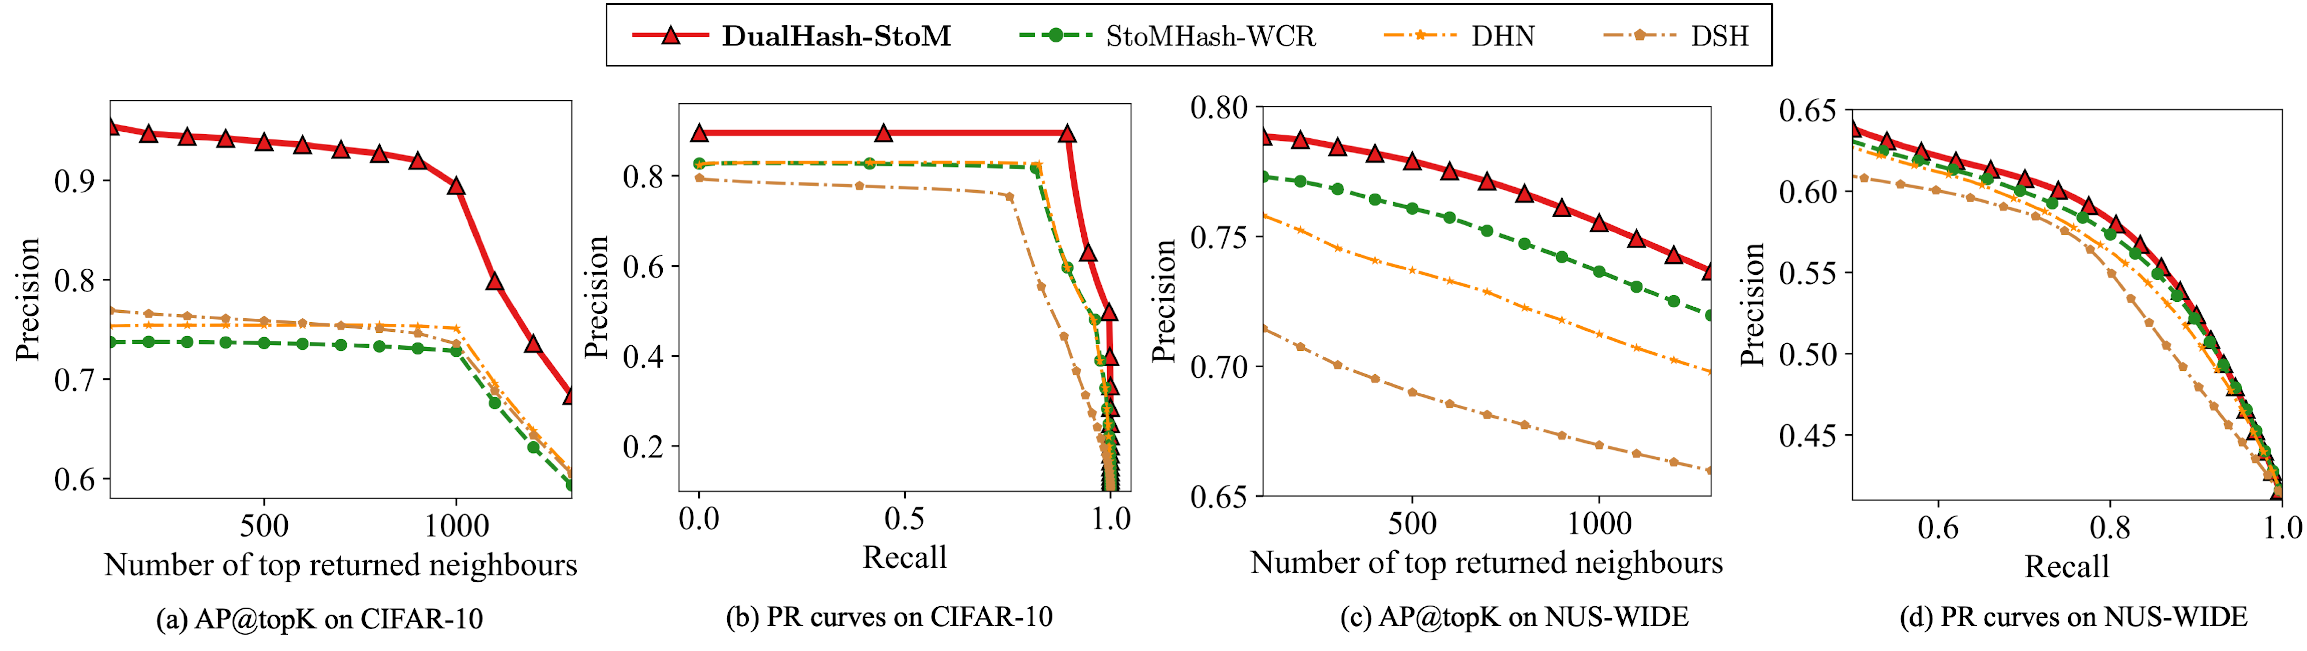
\includegraphics[width=0.95\textwidth]{results_images/ex3_testing_2datasets.pdf}
    \caption{Retrieval performance comparison of DualHash-StoM and three baselines with 64 bits on CIFAR-10 and NUS-WIDE datasets. (a), (c): AP@topK results;  (b), (d): PR curves.}
    \label{fig:ex3_testing_2datasets}
    \vspace{-1ex}
\end{figure*}
Furthermore, \Cref{fig:ex3_testing_2datasets} displays AP@topK results and PR curves
with 64-bit codes on both datasets. DualHash-StoM consistently outperforms all
comparison methods by large margins in AP@topK. For PR curves, DualHash-StoM
demonstrates superior performance at lower recall levels, making it especially well-suited
for precision-critical image retrieval systems.

% \end{document}

\clearpage
\onecolumn 
\section*{Supplementary Material B}
% This supplementary material provides useful definitions and propositions, necessary lemmas with detailed proofs, and the complete derivations for the main theoretical results and parameters presented in the primary work.
\section{Preliminaries}
\label{Appendix: Preliminaries and notations}
% The proximal mapping admits the following
% properties.
% \begin{proposition}[Properties of proximal operators
% \cite{Rockafellar1998VariationalA}]
%     Let $f : \mathbb{R}^{q}\rightarrow \mathbb{R}\cup \{+\infty\}$ be proper and
%     closed. Then, the following holds.
%     \begin{enumerate}[label=(\roman{*})]
%         \item The set $\operatorname{prox}_{\tau f}(\bx)$ is nonempty and compact
%             for any $\bx \in \mathbb{R}^{q}$ and $\tau > 0$.

%         \item If $f$ is convex, then $\operatorname{prox}_{\tau f}(\bx)$
%             contains exactly one value for any $\bx \in \mathbb{R}^{q}$ and
%             $\tau > 0$.
%     \end{enumerate}
% \end{proposition}

We introduce the following definitions related to subdifferentials.
\begin{definition}[Subdifferentials \cite{Rockafellar1998VariationalA}]
    \label{definition: subgradient} Let $f : \mathbb{R}^{q}\to (-\infty, +\infty
    ]$ be a proper closed function.
    \begin{enumerate}[label=(\roman{*})]
        \item For a given $\bx \in \operatorname{dom}f$, the Fréchet
            subdifferential, or simply of $f$ at $\bx$, written
            $\hat{\partial}f(\bx)$, is the set of all vectors $\bu \in \mathbb{R}
            ^{q}$ that satisfy
            \[
                \liminf_{\by \neq \bx, \by \to \bx}\frac{f(\by) - f(\bx) -
                \langle \bu, \by - \bx \rangle}{\|\by - \bx\|}\geq 0.
            \]

        \item The limiting-subdifferential, or simply the subdifferential, of $f$
            at $\bx$, written $\partial f(\bx)$, is defined through the following
            closure process
\[
\partial f(\bx) := \{ \bu \in \mathbb{R}^{q}: \exists \bx^{k}\to \bx, f(\bx^{k}) \to f(\bx), \bu^{k}\in \hat{\partial}f(\bx^{k}) \to \bu \text{ as }k \to \infty \}.
\]
    \end{enumerate}
\end{definition}
Notionally, $\hat{\partial}f(\bx) = \partial f(\bx) = \emptyset$ for all $\bx \notin
\operatorname{dom}(f)$. From definition \cref{definition: subgradient} it
follows that $\hat{\partial}f(\bx) \subset \partial f(\bx)$ for all
$\bx \in \operatorname{dom}(f)$. Moreover, $\hat{\partial}f(\bx)$ is closed
convex while $\partial f(\bx)$ is merely closed. In particular, if $f$ is convex,
then
\[
    \hat{\partial}f(\bx) = \partial f(\bx) = \{ \bd \in \mathbb{R}^{q}\mid f(\by
    ) \geq f(x) + \langle \bd, \by - \bx \rangle ,\,\forall \by \in \mathbb{R}
    ^{q}\}.
\]
The following proposition lists several useful properties of subgradients.
\begin{proposition}[Properties of subdifferential\cite{Rockafellar1998VariationalA}]
    Let $f : \mathbb{R}^{q_1}\rightarrow (-\infty, \infty]$ and $g : \mathbb{R}^{q_2}
    \rightarrow (-\infty, \infty]$ be proper and lower semicontinuous, and let
    $h : \mathbb{R}^{q_1}\rightarrow \mathbb{R}$ be continuously differentiable.
    Then the following results hold:
    \begin{enumerate}[label=(\roman{*})]
        \item For any $\bx \in \mathbb{R}^{q_1}$, we have
            $\hat{\partial}f(\bx) \subseteq \partial f(\bx)$. If, in addition, $f$
            is convex, we have $\hat{\partial}f(\bx) = \partial f(\bx)$.

        \item For $\bx \in \mathbb{R}^{q_1}$ with $f(\bx) < \infty$, it holds
           \[
\begin{aligned}
    \hat{\partial}(f + h)(\bx) &= \hat{\partial}f(\bx) + \nabla h(\bx) \quad \text{and}\\
    \partial (f + h)(\bx) &= \partial f(\bx) + \nabla h(\bx).
\end{aligned}
\]
        \item If $\sigma(\bx_{1}, \bx_{2}) = f_{1}(\bx_{1}) + f_{2}(\bx_{2})$,
            then
            \[
                \begin{pmatrix}
                    \hat{\partial}_{\bx_1}f_{1}(\bar{\bx}_{1}) \\
                    \hat{\partial}_{\bx_2}f_{2}(\bar{\bx}_{2})
                \end{pmatrix}
                \subseteq \hat{\partial}\sigma(\bar{\bx}_{1}, \bar{\bx}_{2}) \quad
                \text{and}\quad
                \begin{pmatrix}
                    \partial_{\bx_1}f_{1}(\bar{\bx}_{1}) \\
                    \partial_{\bx_2}f_{2}(\bar{\bx}_{2})
                \end{pmatrix}
                \subseteq \partial \sigma(\bar{\bx}_{1}, \bar{\bx}_{2}).
            \]
    \end{enumerate}
\end{proposition}
For \Cref{alg:our_algorithm_sgdm}, the key relationships among iterates via the momentum acceleration framework in \eqref{Eq: the update of x in SGDM} are established as follows.
\begin{proposition}[Lemma 5.2 in \cite{InertialProximalAlternating}]
    \label{Pp: relations of xyz} Let $\{\bx^{k}\}_{k \in \mathbb{N}}$,
    $\{\by^{k}\}_{k \in \mathbb{N}}$, and $\{\bz^{k}\}_{k \in \mathbb{N}}$ be sequences
    generated by \eqref{Eq: the update of x in SGDM}. For all $k \in \mathbb{N}$,
    we have:
    \begin{enumerate}[label=(\roman{*})]
        \item $\|\bx^{k}- \by^{k}\|^{2}= \alpha_{k}^{2}\|\bx^{k}- \bx^{k-1}\|^{2}$,

        \item $\|\bx^{k}- \bz^{k}\|^{2}= \beta_{k}^{2}\|\bx^{k}- \bx^{k-1}\|^{2}$,

        \item $\|\bx^{k+1}- \by^{k}\|^{2}\geq 2(1 - \alpha_{k})\|\bx^{k+1}- \bx^{k}
            \|^{2}+ 2\alpha_{k}(\alpha_{k}- 1)\|\bx^{k}- \bx^{k-1}\|^{2}$.
    \end{enumerate}
\end{proposition}
% For  \Cref{alg:our_algorithm_sgdm},  we establish key relationships among iterates via the momentum acceleration framework in \eqref{Eq: the update of x in SGDM}.
% \begin{proposition}[Lemma 5.2 in \cite{InertialProximalAlternating}]
%     \label{Pp: relations of xyz} Let $\{\bx^{k}\}_{k \in \mathbb{N}}$,
%     $\{\by^{k}\}_{k \in \mathbb{N}}$, and $\{\bz^{k}\}_{k \in \mathbb{N}}$ be sequences
%     generated by \eqref{Eq: the update of x in SGDM}. For all $k \in \mathbb{N}$,
%     we have:
%     \begin{enumerate}[label=(\roman{*})]
%         \item $\|\bx^{k}- \by^{k}\|^{2}= \alpha_{k}^{2}\|\bx^{k}- \bx^{k-1}\|^{2}$,

%         \item $\|\bx^{k}- \bz^{k}\|^{2}= \beta_{k}^{2}\|\bx^{k}- \bx^{k-1}\|^{2}$,

%         \item $\|\bx^{k+1}- \by^{k}\|^{2}\geq 2(1 - \alpha_{k})\|\bx^{k+1}- \bx^{k}
%             \|^{2}+ 2\alpha_{k}(\alpha_{k}- 1)\|\bx^{k}- \bx^{k-1}\|^{2}$.
%     \end{enumerate}
% \end{proposition}
% For \Cref{alg:our_algorithm_storm}, we employ the STORM (STochastic Recursive Momentum)  variance reduction estimator \cite{cutkoskyMomentumBasedVarianceReduction2019}.
% In stochastic optimization problems where $F(\bx) = \mathbb{E}_{\xi}[F(\bx;\xi)]$ with $\xi \in \Xi$, standard momentum methods use
% \[
%     \bd^{k}= \rho_{k}\nabla F(\bx^{k}, \xi^{k}) + (1 - \rho_{k}) \bd^{k-1}, \text{
%     where }\rho_{k}\in [0, 1],
% \] yielding a biased estimate of $\nabla F(\bx^{k})$. 
% STORM adds a
% correction term, $(1 - \rho_{k}) (\nabla F(\bx^{k}, \xi^{k}) - \nabla F(\bx^{k-1}
% , \xi^{k})$, resulting in:
% \[
%     \begin{aligned}
%          & \bd^{k}=\left\{\begin{array}{ll}\nabla F\left(\bx^{k}, \xi^{k}\right), & \text{if } k=1, \\ \nabla F\left(\bx^{k}, \xi^{k}\right) + \left(1-\rho_k\right)\left( \bd^{k-1} - \nabla F\left(\bx^{k-1}, \xi^{k}\right) \right), & \text{if } k>1,\end{array}\right. \\
%          & \bx^{k+1}=\bx^{k}-\eta_{k}\bd^{k}.
%     \end{aligned}
% \]
% This exploits the smoothness of $F(\cdot, \xi)$, leading to efficient
% variance reduction. When $\rho_{k}= 1$, $\bd^{k}$ reduces to vanilla mini-batch SGD. We set $\rho_{k}\in (0,1)$ for $k \geq 1$ in \Cref{alg:our_algorithm_storm}.
% \newpage
\section{Discussions on \Cref{Ass: main assumptions}(ii) in \Cref{Section: Convergence analysis}}

\label{Appendix: discussion on assumptions} 
This section verifies that the smoothness constant $L_F$ in \Cref{Ass: main assumptions}(ii) is independent of the sample size $n$, which is essential for our convergence analysis.

For the smooth properties of mappings in our problem, we consider the nonlinear mapping
$\mathcal{D}(\bx) = (\bD_{1}(\bx), \ldots, \bD_{n}(\bx))$ from $\mathcal{X}\subseteq
\RR^{d_{\bx}}$ to $\RR^{n \times d}$, and make the following assumption:

\begin{assumption}
    [Properties of $\mathcal{D}$] \label{Ass: the properties of D} Suppose there
    exist constants $L_{\mathcal{D}},\, L_{\nabla \mathcal{D}}>0$ such that for any
    $\bx, \bx' \in \mathcal{X}$:
    $\|\mathcal{D}(\bx) - \mathcal{D}(\bx')\| \leq L_{\mathcal{D}}\|\bx - \bx'\|$
    and
    $\|\nabla \mathcal{D}(\bx) - \nabla \mathcal{D}(\bx')\| \leq L_{\nabla
    \mathcal{D}}\|\bx - \bx'\|$.
\end{assumption}

Combining \Cref{Ass: main assumptions}(i) and \Cref{Ass: the properties of D},
we can establish that there exist constants
$C_{\mathcal{D}}, G_{\mathcal{D}}, C_{\mathcal{D}B}> 0$ such that:
\[
    \|\mathcal{D}(\bx)\| \leq C_{\mathcal{D}}, \, \|\nabla \mathcal{D}(\bx)\|
    \leq G_{\mathcal{D}}, \, \text{and}\quad \|\mathcal{D}(\bx) - \bB\| \leq C
    _{\mathcal{D}B}.
\]
Based on these assumptions, we can establish the smoothness properties of the composite
function $F$. First, we observe that $P(\bx, \bB)$ is $\frac{\gamma}{n}$-smooth with
respect to $\bB$ and $\frac{\gamma}{n}(L_{\nabla \mathcal{D}}(C_{\mathcal{D}}+ C_{\bB}
) + G_{\mathcal{D}}L_{\mathcal{D}})$-smooth with respect to $\bx$. Combining
these properties, $P(\bx, \bB)$ has an overall smoothness constant:
\[
    L_{s}= \frac{\gamma}{n}\sqrt{2\max\{L^{2}_{\nabla \mathcal{D}}C^{2}_{\mathcal{D}B}+
    (2G_{\mathcal{D}}^{2}+ 1)L^{2}_{\mathcal{D}}, 2G_{\mathcal{D}}^{2}+ 1\}}= \mathcal{O}
    (1)
\]

Consequently, $F(\bx, \bB)$ is $L_{F}$-smooth with respect to $(\bx, \bB)$, where
$L_{F}= \mathcal{O}(1)$. An important observation is that, despite $C_{\mathcal{D}}$,
$G_{\mathcal{D}}$ and $C_{\mathcal{D}B}$ potentially being
$\mathcal{O}(\sqrt{n})$, the overall smoothness constant $L_{F}$ remains independent
of the sample size $n$, which is crucial for our convergence analysis.
% This smoothness property implies the following descent lemma for $F$ with
% respect to $\bx$ and $\bB$:
% \begin{align}
% \label{Eq: F smoothness with x}
%     F(\bx', \bB) \leq F(\bx, \bB) + \langle \nabla_{\bx}F(\bx, \bB), \bx' -\bx\rangle
%     + \frac{L_{F}}{2}\| \bx - \bx'\|^{2}
% \end{align}
% for any $\bB \in \calB$; and similarly for $\bB$:
% {\small 
% \begin{align}
% \label{Eq: F smoothness with B}
%     F(\bx, \bB') \leq F(\bx, \bB) + \langle \nabla_{\bB}F(\bx, \bB), \bB' -\bB\rangle
%     + \frac{L_{F}}{2}\| \bB - \bB'\|^{2}
% \end{align}} for any $\bx \in \calX$.

\section{Complexity analysis of DualHash-StoM (\texorpdfstring{\Cref{alg:our_algorithm_sgdm}}{Algorithm 1})}
\label{Appendix: the complexity analysis of DualHash-StoM}
We adopt the notation and intermediate results from \Cref{Section: Convergence analysis}.
Let us introduce the notation that will be used throughout our analysis:
\begin{align*}
    \bxi^{k}                & = \{\xi_{j}^{k}, j \in \calJ_{k}\},        & \text{(mini-batch at iteration $k$)}                 \\
    \bxi^{[k]}              & = \{\bxi^{1}, \bxi^{2}, \ldots, \bxi^{k}\}, & \text{(history of mini-batches up to iteration $k$)} \\
    \EE_{\bxi^{[k]}}[\cdot] & = \EE [ \cdot | \bxi^{[k]}] .              & \text{(conditional expectation given history)}
\end{align*}

For $\bd^{k}\in \partial \calL(\bx^{k}, \bB^{k}, \bm{\Lambda}^{k})$, let us
denote $\bd^{k}= (\bd_{\bx}^{k}, \bd_{\bB}^{k}, \bd_{\bm{\Lambda}}^{k})$ and
\begin{align}
    % \label{Eq: the components of the subgradient}
    \begin{cases}&\bd_{\bx}^{k}= \nabla_{\bx}F(\bx^{k}, \bB^{k}),\\&\bd_{\bB}^{k}= \nabla_{\bB}F(\bx^{k}, \bB^{k}) + \bm{\Lambda}^{k}, \\&\bd_{\bm{\Lambda}}^{k}= \bB^{k}- \calG_{\bm{\Lambda}}^{k},\end{cases} \notag
\end{align}
where $\calG_{\bm{\Lambda}}^{k}\in \partial h^{*}(\bm{\Lambda}^{k})$.
We first present a lemma concerning a property of a continuously differentiable function with a Lipschitz continuous gradient, followed by a proposition that details the interrelations among the sequences $\{\bx^{k}\}_{k \in \NN},\, \{\bm{y}^{k}\}_{k \in \NN},\, \{\bm{z}^{k}\}_{k \in \NN}$ generated by the algorithm.
% In particular, $\Delta_{\bx}^{k}$ and $\Delta_{\bB}^{k}$ are as defined therein, and we refer to \Cref{Lemma: dual boundedness} and \Cref{Lemma: One-iteration progress of B and Lambda} for the bounds on dual variable dynamics and one-iteration Lagrangian progress on $\bB$ and $\bLmbd$. The gradient error is defined as $\be^{k}= \bG^{k}- \nabla_{\bx}F(\bz^{k}, \bB^{k})$, satisfying $\EE_{\bxi^{[k]}}[\|\be^{k}\|^{2}] \leq \sigma^{2}/b_{k}$ under \Cref{Ass: main assumptions}~(iii).
\begin{lemma}
    \label{Lemma: auxiliary lemma for f} Let $f(\bx): \mathbb{R}^{q}\rightarrow \mathbb{R}$
    be a continuously differentiable function with $L$-lipschitz continuous gradient.
    Then, for any $\bx,\, \by,\,\bz \in \mathbb{R}^{q}$ and any $\bx^{+}\in \mathbb{R}
    ^{q}$ defined by
    \[
        \bx^{+}= \by - \eta \nabla f(\bz), \hspace{5pt}\eta > 0,
    \]it holds that
    \begin{align}
        \label{Eq: auxiliary lemma for f}f(\bx^{+}) \leq f(\bx) + \langle \nabla f(\bx) - \nabla f(\bz), \bx^{+}- \bx \rangle + \frac{L}{2}\|\bx^{+}- \bx\|^{2}+ \frac{1}{2\eta}\|\bx - \by\|^{2}- \frac{1}{2\eta}\|\bx^{+}- \by\|^{2}.
    \end{align}
\end{lemma}
\begin{proof}
    By the definition of $\bx^{+}$, we find that
    \[
        \bx^{+}= \argmin\limits_{\bu \in \mathbb{R}^d}\{ \langle \nabla f(\bz), \bu
        - \by \rangle + \frac{1}{2\eta}\| \bu - \by\|^{2}\},
    \]
    and hence, in particular, by taking $\bu = \bx$, we obtain
    \begin{align*}
        0 \leq \langle \nabla f(\bz), \bx - \bx^{+}\rangle + \frac{\tau}{2}\| \bx - \by\|^{2}- \frac{1}{2\eta}\| \bx^{+}- \by\|^{2}.
    \end{align*}
    Invoking the descent lemma for a smooth function yields the result. 
\end{proof}
\subsection{Proof of \Cref{Lemma: One-iteration progress of x in SGDM}}
\label{Subsubsec: proof x progress SGDM}

\begin{proof}
    Recalling the equivalent relation:
    \begin{align}
        \label{Eq: the update of x one progress in StoM}\mathcal{L}(\bx^{k+1}, \bm{B}^{k}, \bm{\Lambda}^{k}) - \mathcal{L}(\bx^{k}, \bm{B}^{k}, \bm{\Lambda}^{k}) = F(\bx^{k+1}, \bm{B}^{k}) - F(\bx^{k}, \bm{B}^{k}).
    \end{align}
    Then, applying the smoothness of $F$ with respect to $\bx$ and \eqref{Eq: auxiliary lemma for f}
    yields
    \begin{align}
        \label{Eq: the update of theta core}F(\bx^{k+1}, \bm{B}^{k}) \leq & F(\bx^{k}, \bm{B}^{k}) + \langle \nabla_{\bx}F(\bx^{k}, \bm{B}^{k}) - \bG^{k}, \bx^{k+1}- \bx^{k}\rangle \notag                              \\
        +                                                                 & \frac{L_{F}}{2}\|\bx^{k+1}- \bx^{k}\|^{2}+ \frac{1}{2\eta_{k}}\|\bx^{k}- \bm{y}^{k}\|^{2}- \frac{1}{2\eta_{k}}\|\bx^{k+1}- \bm{y}^{k}\|^{2}.
    \end{align}
    For the inner product term in \eqref{Eq: the update of theta core}, using
    the facts that
    $\langle a, b \rangle \leq \frac{s}{2}\|a\|^{2}+ \frac{1}{2s}\|b\|^{2}$ for
    any $s > 0$ and $\| a - c \|^{2}\leq 2\|a - b \|^{2}+ 2\|b -c\|^{2}$ yields
    { \begin{align}\label{Eq: Inner product for theta}&\langle \nabla_{\bx}F(\bx^{k}, \bm{B}^{k}) - \bG^{k}, \bx^{k+1}- \bx^{k}\rangle \notag \\ \leq&\,\frac{s}{2}\|\bx^{k+1}- \bx^{k}\|^{2}+ \frac{1}{s}\|\nabla_{\bx}F(\bx^{k}, \bm{B}^{k}) - \nabla_{\bx}F(\bm{z}^{k}, \bm{B}^{k}) \|^{2}+ \frac{1}{s}\|\nabla_{\bx}F(\bm{z}^{k}, \bm{B}^{k}) - \bG^{k}\|^{2}\notag \\ \leq&\, \frac{s}{2}\|\bx^{k+1}- \bx^{k}\|^{2}+ \frac{L^{2}_{F}}{s}\|\bx^{k}- \bm{z}^{k}\|^{2}+ \frac{1}{s}\|\nabla_{\bx}F(\bm{z}^{k}, \bm{B}^{k}) - \bG^{k}\|^{2}.\end{align}}
    Setting $s = L_{F}$ in \eqref{Eq: Inner product for theta} and substituting into
    \eqref{Eq: the update of theta core}, then applying \cref{Pp: relations of xyz},
    we obtain
    \begin{align}
        F(\bx^{k+1}, \bm{B}^{k}) & \leq F(\bx^{k}, \bm{B}^{k}) - (\frac{1 - \alpha_{k}}{\eta_{k}}- 2L_{F})\frac{\|\bx^{k+1}- \bx^{k}\|^{2}}{2}\notag                                                                                           \\
                                 & +\,(\frac{\alpha_{k}}{\eta_{k}}+ 2L_{F}\beta_{k}^{2})\frac{\|\bx^{k}- \bx^{k-1}\|^{2}}{2}+ \frac{1}{L_{F}}\|\nabla_{\bx}F(\bm{z}^{k}, \bm{B}^{k}) - \bG^{k}\|^{2}. \label{Eq: the update of x of L in StoM}
    \end{align}
    Substituting \eqref{Eq: the update of x of L in StoM} into \eqref{Eq: the update of x one progress in StoM}
    yields \eqref{Eq: One-iteration progress of x in SGDM} and completes the proof.
    
    % \begin{align}
    %     \label{item: x}
    %     &\mathcal{L}(\bx^{k+1}, \bm{B}^k, \bm{\Lambda}^k) -\mathcal{L}(\bx^k, \bm{B}^k, \bm{\Lambda}^k)  \notag \\
    %     \leq &\,-(\frac{1 - \alpha_k}{\eta_k}- 2L_F) \frac{ \|\bx^{k+1} - \bx^k \|^2}{2}
    %     + (\frac{\alpha_k}{\eta_k}+ 2L_F\beta_k^2) \frac{\|\bx^k - \bx^{k-1} \|^2}{2} \notag \\
    %     \quad&+ \frac{1}{L_F} \|\nabla_{\bx} F(\bm{z}^k, \bm{B}^k) - \bG^k \|^2.
    % \end{align} 
\end{proof}
\subsection{Proof of \Cref{Lemma: approximate sufficient descent property in SGDM}}
\label{Subsubsec: proof descent SGDM}

\begin{proof}
    Substituting one-iteration progress \eqref{Eq: One-iteration progress of x in SGDM}
    and \eqref{item: B and Lambda} into \eqref{Eq: One-iteration progress decomposition}
    , we obtain
    \begin{align}
        \label{Eq: One-iteration progress in sgdm} & \calL (\bx^{k+1}, \bB^{k+1}, \bLmbd^{k+1}) - \calL (\bx^{k}, \bB^{k}, \bLmbd^{k}) \notag                                                                                                   \\
        \leq \,                                    & K_{1}\Delta_{\bB}^{k+2}- K_{2}\Delta_{\bB}^{k+1}+ K_{3}\Delta_{\bB}^{k}+ K_{4}\Delta_{\bx}^{k+2}- (K_{5}- K_{3})\Delta_{\bx}^{k+1}+ K_{6}\Delta_{\bx}^{k}+ \frac{1}{L_{F}}\|\be^{k}\|^{2}.
    \end{align}
    Applying the definition of $\Psi_m$ from \eqref{Eq: the Lyapunov function in SGDM}
    to \eqref{Eq: One-iteration progress in sgdm}, rearranging, and taking the
    conditional expectation on both sides, we obtain
    \begin{align}
        \label{the descent property of Lyapunov func in SGDM first} & \EE_{\bxi^{[k+1]}}\left[\Psi_m(\mathcal{Q}^{k+1})\right] - \EE_{\bxi^{[k]}}\left[\Psi_m(\mathcal{Q}^{k})\right]\notag                                                                               \\
        \leq                                                        & - (C_{1}- K_{1}) \EE_{\bxi^{[k+1]}}[\Delta_{\bm{B}}^{k+2}] -(K_{2}- C_{1}- C_{2}) \EE_{\bxi^{[k+1]}}[\Delta_{\bm{B}}^{k+1}] - (C_{2}- K_{3}) \EE_{\bxi^{[k]}}[\Delta_{\bm{B}}^{k}] \notag                     \\
                                                                    & - (C_{3}-K_{4}) \EE_{\bxi^{[k+1]}}[\Delta_{\bx}^{k+2}]- (K_{5}-K_{3}-C_{3}-C_{4}) \EE_{\bxi^{[k+1]}}[\Delta_{\bx}^{k+1}] - (C_{4}- K_{6}) \EE_{\bxi^{[k]}}[\Delta_{\bx}^{k}] + \frac{\sigma^{2}}{b_{k}L_{F}}.
    \end{align}
    Then substituting the values of coefficients in \eqref{Eq: the coefficients of the Lyapunov function in SGDM}
    and parameter conditions \eqref{Eq: the parameters conditions of dualhash-sgdm in suppl}
    into \eqref{the descent property of Lyapunov func in SGDM first}, we derive
    \begin{align*}
             & \EE_{\bxi^{[k+1]}}\left[\Psi_m(\mathcal{Q}^{k+1})\right] - \EE_{\bxi^{[k]}}\left[\Psi_m(\mathcal{Q}^{k})\right] \nonumber                                                                                                                                                        \\
        \leq & \, -C_{\bB}\left( \EE_{\bxi^{[k+1]}}\left[\Delta_{\bB}^{k+1}\right] + \EE_{\bxi^{[k]}}\left[\Delta_{\bB}^{k}\right] \right) -C_{\bx}\left( \EE_{\bxi^{[k+1]}}\left[\Delta_{\bm{x}}^{k+1}\right]+ \EE_{\bxi^{[k]}}\left[\Delta_{\bm{x}}^{k}\right] \right) + \frac{\sigma^{2}}{b_{k}L_{F}}.
    \end{align*}Taking the full expectation of both sides leads to \eqref{Eq: the descent coefficients of potential function in SGDM},
    thereby completing the proof. 
\end{proof}
The technical proof that the coefficients of $\Psi_m$ in \eqref{Eq: the coefficients of the Lyapunov function in SGDM} and the descent constants $C_{\bB}$, $C_{\bx}$ are indeed positive is given as follows.
\begin{lemma}[Positivity of Lyapunov related coefficients]
    \label{lem:lyapunov-coef-positivity} If parameter conditions \eqref{Eq: the parameters conditions of dualhash-sgdm in suppl}
    hold, then the following inequalities are satisfied:
    \begin{align}
        % \label{Eq: the positive coefficients}
        \begin{cases}K_{5}- K_{3}- C_{3}- C_{4}\geq \nu C_{4}, \\ C_{4}- K_{6}\geq \nu C_{4},\\ C_{4}> 0,\\ C_{\bB}> 0 ,\\ C_{2},\, C_{1}> 0, \\ C_{\bx}> 0.\end{cases} \notag
    \end{align}
\end{lemma}
\begin{proof}
    For $K_{5}- K_{3}- C_{3}- C_{4}$ and $C_{4}- K_{6}$ in \eqref{the descent property of Lyapunov func in SGDM first},
    we obtain by straightforward computations by choosing some $\nu > 0$,
    {\begin{align}
        K_{5}- K_{3}- C_{3}- C_{4}
        &= \frac{1 - \alpha_{k}}{\eta_{k}}- \bar{L}_{F}- (1 + \nu)C_{4}+ \nu C_{4}\notag\\
        &= (1 - \alpha_{k})\left(\frac{1}{\eta_{k}}- \frac{\bar{L}_{F}+ (1 + \nu)C_{4}}{1 - \alpha_{k}}\right) + \nu C_{4}\notag \\
        &\geq \nu C_{4}. \notag % \label{Eq: the scaling of the delta1}
    \end{align}}
    where the last inequality follows from $\alpha_{k}= \alpha$ and
    $\frac{1}{\eta_{k}}= \frac{\bar{L}_{F}+ (1 + \nu)C_{4}}{1 - \alpha}$. Then,
    one has
    \begin{align}
        C_{4}- K_{6} & = C_{4}- \frac{\alpha}{\eta_{k}}- 2L_{F}\beta_{k}^{2}\notag                                                                                                                                   \\
                     & = \frac{1}{1 - \alpha}\left( (1 - \alpha)C_{4}- \alpha\bar{L}_{F}- (1 + \nu)C_{4}\alpha - 2L_{F}\beta^{2}(1 - \alpha) \right)\notag                                                           \\
                     & \geq \frac{1}{1 - \alpha}\left( (1 - 2\alpha - \nu)C_{4}- \alpha \left(\bar{L}_{F}+ \frac{2L_{F}\beta^{2}}{\alpha}\right) \right) + \nu C_{4}+ \frac{2L_{F}\beta^{2}\alpha}{1 - \alpha}\notag \\
                     & \geq \nu C_{4}. \notag % \label{Eq: the scaling of the delta2}
    \end{align}
    where the last inequality follows from $\alpha \in (0, \frac{1 - \nu}{2})$
    and
    $C_{4}= \frac{\bar{L}_{F}+ \frac{2L_F \beta^2}{\alpha}}{1 - 2\alpha - \nu}> 0$.
    We rearrange $\frac{1}{\eta_{k}}$ using the definition of $C_{4}$ and obtain
    $\eta_{k}= \frac{\eta}{L_{F}}$ where $\eta = \frac{(1 - 2\alpha - \nu)/2}{\frac{\bar{L}_{F}}{L_{F}}
    + \frac{(1 + \nu)\beta^{2}}{(1 - \alpha)\alpha}}$.

    Next, we verify that the coefficients of $\Psi_m$ satisfying \eqref{Eq: the coefficients of the Lyapunov function in SGDM}
    and $\tau$ satisfying \eqref{Eq: the parameters conditions of dualhash-sgdm in suppl}
    ensure that $C_{\bB},\, C_{\bx}> 0$. Let us denote $t = \tau L_{F}$. Choosing
    $\delta>0$, we have
    \begin{align*}
        C_{\bB}= \frac{L_{F}}{2}\left(\frac{2 - 6\delta}{t}- \left(3\delta + \frac{1}{\delta}\right)t- (6\delta+1) \right) \geq 0.
    \end{align*}
    If we choose $\delta = \frac{1}{6}> 0$, then
    \[
        \frac{2}{L_{F}}C_{\bB}= \frac{2}{t}- \frac{13}{2}t - 2 \geq 0.
    \]
    By selecting
    $\tau \in \left(0, 6(\frac{\sqrt{30}-2}{13})\delta \frac{1}{L_{F}}\right]$, it
    is sufficient to ensures $C_{\bB}> 0$, and consequently, $C_{2},\,C_{1}> 0$.
    Therefore, for some $\delta >0$, setting
    $\tilde{\delta}= c_{\delta}\delta^{2}$ and ensuring
    $\tau^{2}L_{F}^{2}\leq \tilde{\delta}$ guarantee positive coefficients for
    $\Psi_m$ in \eqref{Eq: the coefficients of the Lyapunov function in SGDM}
    and $C_{\bB}, \, C_{\bx}>0$. 
\end{proof}
We then derive an upper error bound on $\text{dist}^{2}(\bm{0}, \partial \calL(\bx^{k}, \bB^{k}, \bm{\Lambda}^{k}))$ based on
\begin{align}
    \label{Eq: the stationarity error bound in proof}\text{dist}^{2}(\bm{0}, \partial \calL(\bx^{k}, \bB^{k}, \bm{\Lambda}^{k})) \leq \| \bd^{k}\|^{2}=\|\bd_{\bx}^{k}\|^{2}+ \| \bd_{\bB}^{k}\|^{2}+ \| \bd_{\bm{\Lambda}}^{k}\|^{2}.
\end{align}

\begin{lemma}[Stationarity error bound]
    \label{Lemma: Stationarity error bound in SGDM} Under \Cref{Ass: main assumptions},
    for \(\forall\) $k \geq 1$, it holds that
    \begin{align}\label{Eq: the stationarity error bound in SGDM Lemma}
        \EE [\text{dist}^{2}(\bm{0}, \partial \calL(\bx^{k}, \bB^{k}, \bm{\Lambda}^{k}))] \leq S_{1}\EE[ \Delta_{\bB}^{k+1}] + S_{2}\EE[ \Delta_{\bB}^{k}] + S_{3}^{k}\EE[ \Delta_{\bm{x}}^{k+1}] + S_{4}^{k}\EE [\Delta_{\bm{x}}^{k}] + \frac{3\sigma^{2}}{b_{k}L_{F}},
    \end{align}
    where the coefficients are given by
    \begin{align}
        \label{Eq: the coefficients of stationarity error bound in SGDM}\begin{cases}S_{1}&= 4\tau^{-2}+ 12,\\ S_{2}&= 4(1 + 3 (1 + \tau L_{F})^{2}),\\ S_{3}^{k}&= 4(\eta_{k}^{-2}+ L_{F}^{2}+ 3 (\tau L_{F})^{2}),\\ S_{4}^{k}&= 6 ( L_{F}\beta_{k}^{2}+ 6 \eta_{k}^{-2}\alpha_{k}^{2}).\end{cases}
    \end{align}
\end{lemma}
% \begin{proof}
% For estimating \(\bd_{\bx}^k\), using the optimality condition of \(\bx^k\), we obtain
% \begin{align}
%     &\|\bd_{\bx}^k\|^2 \notag \\
%     =&\,\|\nabla_{\bx} F(\bx^k, \bm{B}^k) \|^2  \notag\\
%     =&\,\eta_k^{-2} \left\| \eta_k \nabla_{\bx} F(\bx^k, \bm{B}^k) + 0\right\|^2 \notag \\
%     =&\, \eta_k^{-2}  \left\|\eta_k\left( \nabla_{\bx} F(\bx^k, \bm{B}^k) - \bG^k \right) + \bm{y}^k - \bx^{k+1} \right\|^2 \notag \\
%     =&\,\eta_k^{-2} \bigg\|\eta_k\Big(
%     \nabla_{\bx} F(\bx^k, \bm{B}^k) - \nabla_{\bx} F(\bm{z}^k, \bm{B}^k) \notag \\
%     &\qquad + \nabla_{\bx} F(\bm{z}^k, \bm{B}^k)- \bG^k \Big)
%     + \bm{y}^k - \bx^k + \bx^k - \bx^{k+1} \bigg\|^2
%     \label{eq:ineq1} \\
%     \leq&\, 3 \|\nabla_{\bx} F(\bx^k, \bm{B}^k) - \nabla_{\bx} F(\bm{z}^k, \bm{B}^k)\|^2
%     + 3\eta_k^{-2}\|\bx^{k+1} - \bx^k + \bx^k - \bm{y}^k \|^2 \notag \\
%     \quad& + 3 \|\be^k\|^2
%     \label{eq:ineq2} \\
%     \leq&\, 3L_F^2 \|\bx^k - \bm{z}^k \|^2
%     + 6\eta_k^{-2} \left(\|\bx^{k+1} - \bx^k\|^2 + \|\bx^k - \bm{y}^k \|^2\right) \notag \\
%     \quad& + 3 \|\be^k\|^2,
% \end{align} where \eqref{eq:ineq1} is deduced by using the fact that \((a + b+ c)^2 \leq 3(a^2 + b^2 +c^2)\) and \eqref{eq:ineq2} is deduced by the smoothness of \( F(\bx, \bm{B})\) and \((a + b)^2 \leq 2(a^2 + b^2)\).
% Then using \cref{Pp: relations of xyz} concludes
%     \begin{align}
%     \label{Eq: dx}
%     \| \bd_{\bx}^k\| \leq  6( L_F \beta_k^2 + 2 \eta_k^{-2} \alpha_k^2) \Delta_{\bx}^{k} + 12 \eta_k^{-2} \Delta_{\bx}^{k+1} + 3 \| \be^k\|^2
%     \end{align}
%     For estimating  \(\bd^k_{\bB}\), using the optimality condition of \(\bB^k\) and the smoothness of \(F\), we obtain
% \begin{align}
%     \|\bd_{\bB}^k\|^2&= \| \nabla_{\bB} F(\bx^{k+1}, \bB^k)+  \bm{\Lambda}^k + \nabla_{\bB} F(\bx^k, \bB^k) - \nabla_{\bB} F(\bx^{k+1}, \bB^k) \|^2 \notag \\
%                     &= 4 \tau^{-2} \Delta^{k+1}_{\bB}  + 4L_F^2\Delta_{\bx}^{k+1} \label{Eq: dB},
% \end{align} where the last inequality follows from the fact \((a + b)^2 \leq 2(a^2 + b^2)\).

% For estimating \( \|\bd^k_{\bm{\Lambda}}\|^2\),  using the optimality condition of \( \bm{\Lambda}^k \) in \eqref{Eq: the optimality condition of lbda},  we obtain
% \begin{align*}
%         \|\bd^k_{\bm{\Lambda}}\|^2 &\leq 2\tau^{2} \|\bm{\Lambda}^k - \bm{\Lambda}^{k-1} \|^2+ 2\|\bB^{k} - \bB^{k-1}\|^2.
%     \end{align*} Then, substituting \eqref{Eq: dual boundedness} in \cref{Lemma: dual boundedness} into the above inequality yield that
% \begin{align}
% \label{Eq: dLambda}
% \|\bd^k_{\bm{\Lambda}} \|^2 \leq 12 \Delta_{\bB}^{k+1} + 4(1 + 3 (1 + \tau L_F )^2)\Delta_{\bB}^k + 12(\tau L_F)^2\Delta_{\bx}^{k+1} .
% \end{align}
% Then, substituting \eqref{Eq: dx}, \eqref{Eq: dB} and \eqref{Eq: dLambda} into \eqref{Eq: the stationarity error bound in proof} yields \eqref{Eq: the stationarity error bound in SGDM Lemma} and completes the proof. 
% \end{proof}
\begin{proof}
    For estimating $\| \bd_{\bx}^{k}\|^{2}$, using the optimality condition of
    $\bx^{k}$, we obtain
    \begin{align}
             & \|\bd_{\bx}^{k}\|^{2}\notag                                                                                                                                                                                                                   \\
        =    & \,\|\nabla_{\bx}F(\bx^{k}, \bm{B}^{k}) \|^{2}\notag                                                                                                                                                                                           \\
        =    & \,\eta_{k}^{-2}\left\| \eta_{k}\nabla_{\bx}F(\bx^{k}, \bm{B}^{k}) + 0\right\|^{2}\notag                                                                                                                                                       \\
        =    & \, \eta_{k}^{-2}\left\|\eta_{k}\left( \nabla_{\bx}F(\bx^{k}, \bm{B}^{k}) - \bG^{k}\right) + \bm{y}^{k}- \bx^{k+1}\right\|^{2}\notag                                                                                                           \\
        =    & \,\eta_{k}^{-2}\bigg\|\eta_{k}\Big( \nabla_{\bx}F(\bx^{k}, \bm{B}^{k}) - \nabla_{\bx}F(\bm{z}^{k}, \bm{B}^{k}) + \nabla_{\bx}F(\bm{z}^{k}, \bm{B}^{k})- \bG^{k}\Big) + \bm{y}^{k}- \bx^{k}+ \bx^{k}- \bx^{k+1}\bigg\|^{2}\label{eq:d_x_ineq1} \\
        \leq & \, 3 \|\nabla_{\bx}F(\bx^{k}, \bm{B}^{k}) - \nabla_{\bx}F(\bm{z}^{k}, \bm{B}^{k})\|^{2}+ 3\eta_{k}^{-2}\|\bx^{k+1}- \bx^{k}+ \bx^{k}- \bm{y}^{k}\|^{2}+ 3 \|\be^{k}\|^{2}\label{eq:d_x_ineq2}                                                 \\
        \leq & \, 3L_{F}^{2}\|\bx^{k}- \bm{z}^{k}\|^{2}+ 6\eta_{k}^{-2}\left(\|\bx^{k+1}- \bx^{k}\|^{2}+ \|\bx^{k}- \bm{y}^{k}\|^{2}\right) + 3 \|\be^{k}\|^{2},\label{eq:d_x_ineq3}                                                                      
    \end{align}
    where \eqref{eq:d_x_ineq1} is deduced by using the fact that
    $(a + b+ c)^{2}\leq 3(a^{2}+ b^{2}+c^{2})$ and \eqref{eq:d_x_ineq2} is deduced
    by the smoothness of $F(\bx, \bm{B})$ and $(a + b)^{2}\leq 2(a^{2}+ b^{2})$.
    Then applying \Cref{Pp: relations of xyz} to \eqref{eq:d_x_ineq3} concludes
    \begin{align}
        \label{Eq: dx}\| \bd_{\bx}^{k}\|^{2}\leq 6( L_{F}\beta_{k}^{2}+ 2 \eta_{k}^{-2}\alpha_{k}^{2}) \Delta_{\bx}^{k}+ 12 \eta_{k}^{-2}\Delta_{\bx}^{k+1}+ 3 \| \be^{k}\|^{2}.
    \end{align}
    For estimating $\|\bd^{k}_{\bB}\|^{2}$, using the $\bB$-update
    \eqref{Eq: the update of B} and the smoothness of
    $F$, we obtain
    \begin{align}
        \|\bd_{\bB}^{k}\|^{2} & = \| \nabla_{\bB}F(\bx^{k+1}, \bB^{k})+ \bm{\Lambda}^{k}+ \nabla_{\bB}F(\bx^{k}, \bB^{k}) - \nabla_{\bB}F(\bx^{k+1}, \bB^{k}) \|^{2}\notag \\
                              & \leq4 \tau^{-2}\Delta^{k+1}_{\bB}+ 4L_{F}^{2}\Delta_{\bx}^{k+1}\label{Eq: dB},
    \end{align}where the last inequality follows from the fact
    $(a + b)^{2}\leq 2(a^{2}+ b^{2})$.

    For estimating $\|\bd^{k}_{\bm{\Lambda}}\|^{2}$, using the
    $\bm{\Lambda}$-update \eqref{Eq: the update of lambda}, we obtain
\begin{align}
    \|\bd^{k}_{\bm{\Lambda}}\|^{2} & \leq 2\tau^{2}\|\bm{\Lambda}^{k}- \bm{\Lambda}^{k-1}\|^{2}+ 2\|\bB^{k}- \bB^{k-1}\|^{2}. \notag
\end{align}

    Then, substituting \eqref{Eq: dual boundedness in proof} into the above inequality yields that
    \begin{align}
        \label{Eq: dLambda}\|\bd^{k}_{\bm{\Lambda}}\|^{2}\leq 12 \Delta_{\bB}^{k+1}+ 4(1 + 3 (1 + \tau L_{F})^{2})\Delta_{\bB}^{k}+ 12(\tau L_{F})^{2}\Delta_{\bx}^{k+1}.
    \end{align}

    Finally, substituting \eqref{Eq: dx}, \eqref{Eq: dB}, and \eqref{Eq: dLambda}
    into \eqref{Eq: the stationarity error bound in proof}, and taking the full expectation
    on both sides, yields \eqref{Eq: the stationarity error bound in SGDM Lemma},
    completing the proof. 
\end{proof}

% We now establish the convergence rate of \Cref{alg:our_algorithm_sgdm} as follows.
% We set $T$ as the maximum number of iterations and denote 
%     $L_{\Delta}= \frac{\max\{S_{1}, S_{2}\} + \max\{S_{3}, S_{4}\}}{\min\{C_{\bB},
%     C_{\bx}\}}$, $C_{\sigma}= \frac{L_{\Delta}}{L_{F}}+ 3$, and
%     $\Delta_{1}= \Psi_m^{1}- \Psi_m(\mathcal{Q}^{*})$
%     are constants independent of $T$, where \(\Psi_m^{1} = \Psi_m(\calQ^1)\).
% \begin{lemma}[Convergence rate of \Cref{alg:our_algorithm_sgdm}]
%     \label{lemma: convergence rate sgdm} Under the conditions of Lemma \ref{Lemma:
%     approximate sufficient descent property in SGDM}, for any $T \geq 1$, there exists
%     $R$ uniformly selected from $\{2,\ldots,T+1\}$ such that $(\bx^{R}, \bB
%     ^{R}, \bLmbd^{R})$ satisfies \eqref{equ:esp} with
%     \begin{align}
%         \label{Eq: the convergence rate of sgdm}\mathbb{E}[\mathrm{dist}^{2}(0, \partial \mathcal{L}(\bx^{R}, \bB^{R}, \bLmbd^{R}))] \leq \frac{L_{\Delta}\Delta_{1}}{T}+ C_{\sigma}\frac{\sigma^{2}}{b_{k}}.
%     \end{align}
% \end{lemma}
\subsection{Proof of \Cref{lemma: convergence rate sgdm}}
\label{Subsubsec: convergence rate SGDM}
\begin{proof}
    From \eqref{Eq: the stationarity error bound in SGDM Lemma}, we obtain \begin{align}\label{Eq: the stationarity error bound in SGDM rearrange}\mathbb{E}[\mathrm{dist}^{2}(0, \partial \mathcal{L}(\bx^{k}, \bB^{k}, \bLmbd^{k}))] \leq ( \max\{S_{1}, S_{2}\} + \max\{S_{3}, S_{4}\}) \EE [\Delta_{\bB}^{k+1}+ \Delta_{\bB}^{k}+ \Delta_{\bx}^{k+1}+ \Delta_{\bx}^{k}] + \frac{3 \sigma^{2}}{b_{k}L_{F}}.\end{align}
    Similarly, from \eqref{Eq: the descent property of Lyapunov func in SGDM}, we
    obtain
    \[
        \EE [\Psi_m(\mathcal{Q}^{k+1})] - \EE[\Psi_m(\mathcal{Q}^{k})]
        \leq -\min \{ C_{\bB}, C_{\bx}\}\EE[\Delta_{\bB}^{k+1}+ \Delta_{\bB}^{k}+
        \Delta_{\bm{x}}^{k+1}+ \Delta_{\bm{x}}^{k}] + \frac{\sigma^{2}}{b_{k}L_{F}},
    \]
    which yields that
    \[
        \EE[\Delta_{\bB}^{k+1}+ \Delta_{\bB}^{k}+ \Delta_{\bm{x}}^{k+1}+ \Delta_{\bm{x}}
        ^{k}] \leq \frac{1}{\min \{ C_{\bB}, C_{\bx}\}}\left( \EE [\Psi_m(\mathcal{Q}
        ^{k})] - \EE[\Psi_m(\mathcal{Q}^{k+1})] + \frac{\sigma^{2}}{b_{k}L_{F}}
        \right)
    \]
    Substituting this inequality into \eqref{Eq: the stationarity error bound in SGDM rearrange},
    summing over $k = 1, \cdots,T$, and dividing by $T$, we obtain
    \[
        \frac{1}{T}\sumT \mathbb{E}[\mathrm{dist}^{2}(0, \partial \mathcal{L}(\bx
        ^{k}, \bB^{k}, \bLmbd^{k}))] \leq \frac{L_{\Delta}}{T}\sumT
        \left(\EE [\Psi_m(\mathcal{Q}^{k})] - \EE [\Psi_m
        (\mathcal{Q}^{k+1})] \right) + ( 3 + L_{\Delta}) \frac{\sigma^{2}}{b_{k}},
    \], which yields the conclusion. Denoting
    $a_{k}= \mathbb{E}[\mathrm{dist}^{2}(0, \partial \mathcal{L}(\bx^{k}, \bB
    ^{k}, \bLmbd^{k}))]$, we have
    \[
        \frac{1}{T}\sumT a_{k}\leq \frac{L_{\Delta}\Delta_{1}}{T}+ ( 3 + L_{\Delta}
        ) \frac{\sigma^{2}}{b_{k}}.
    \]
    By uniformly selecting $R' \in \{1, \ldots, T\}$ and letting $R = R' + 1$,
    we obtain
    \[
        \mathbb{E}[\mathrm{dist}^{2}(0, \partial \mathcal{L}(\bx^{R}, \bB^{R}
        , \bLmbd^{R}))] \leq \frac{L_{\Delta}\Delta_{1}}{T}+ ( 3 + L_{\Delta}
        ) \frac{\sigma^{2}}{b_{k}},
    \] and complete the proof.
\end{proof}
% From \eqref{Eq: the convergence rate of sgdm}, to achieve $\calO(T^{-1})$
% convergence rate, we need to set $b_{k}= \Theta (T)$. Next, we set
% $b_{k}= b = c_{b}T$ for all $k \geq 1$ in this way and establish the complexity
% results of \Cref{alg:our_algorithm_sgdm} with the parameter conditions \eqref{Eq: the parameters conditions of dualhash-sgdm in suppl}.
\subsection{Proof of \Cref{Theorem: the oracle complexity in SGDM}}
\label{Subsec: proof theorem SGDM}
% \setcounter{proof}{0}
\begin{proof}
    When $b_{k}= b = c_{b}T$, we have
    \[
        \mathbb{E}[\mathrm{dist}^{2}(0, \partial \mathcal{L}(\bx^{R}, \bB^{R}
        , \bLmbd^{R}))] \leq \frac{1}{T}\left( L_{\Delta}\Delta_{1}+ C_{\sigma}
        \frac{\sigma^{2}}{c_{b}}\right).
    \]
    With the conditions on $T$ in \eqref{Eq: the iterate number upper bound of algorithm SGDM},
    this gives
    $\mathbb{E}[\mathrm{dist}^{2}(0, \partial \mathcal{L}(\bx^{R}, \bB^{R}
    , \bLmbd^{R}))] \leq \varepsilon^{2}$. Then, the oracle complexity
    of SFO is
    \[
        \text{Complexity}= (T-1)b_{k}=\calO(T^{2}) = \calO(\varepsilon^{-4}).
    \]
\end{proof}

\section{Complexity analysis of DualHash-StoRM (\texorpdfstring{\Cref{alg:our_algorithm_storm}}{Algorithm 2})}
\label{Appendix: the complexity analysis of DualHash-StoRM}
We adopt the same notation as in \Cref{Appendix: the complexity analysis of DualHash-StoM}. 
\subsection{Proof of \Cref{Lemma: approximate sufficient descent property storm}}
\label{Subsubsec: proof descent STORM}
\begin{proof}
    Substituting the one-iteration progress \eqref{Eq: the recursive relation of L on x}
    and \eqref{Eq: the recursive relation of L on B and Lambda} into \eqref{Eq: One-iteration progress decomposition},
    we obtain
    \begin{align}
        % \label{Eq: the recursive relation of L under VR}
        & \calL (\bx^{k+1}, \bB^{k+1}, \bLmbd^{k+1}) - \calL (\bx^{k}, \bB^{k}, \bLmbd^{k}) \notag                                                                                                        \\
        \leq \,                                          & \frac{s}{2}\| \be^{k}\|^{2}- (-\frac{1}{s}+ 2\eta_{k}^{-1}- L_{F}- K_{3}) \Delta_{\bx}^{k+1}+ K_{1}\Delta_{\bB}^{k+2}+ K_{4}\Delta_{\bx}^{k+2}- K_{2}\Delta_{\bB}^{k+1}+ K_{3}\Delta_{\bB}^{k}. \notag
    \end{align}
    where setting $s = \eta_{k}$ yields
    \begin{align}
             & \calL (\bx^{k+1}, \bB^{k+1}, \bLmbd^{k+1}) - \calL (\bx^{k}, \bB^{k}, \bLmbd^{k}) \nonumber                                                                                                                                          \\
        \leq & \,\frac{\eta_{k}}{2}\| \be^{k}\|^{2}- (\eta_{k}^{-1}- L_{F}- K_{3}) \Delta_{\bx}^{k+1}+ K_{1}\Delta_{\bB}^{k+2}+ K_{4}\Delta_{\bx}^{k+2}- K_{2}\Delta_{\bB}^{k+1}+ K_{3}\Delta_{\bB}^{k}.\label{Eq: One-iteration progress in storm}
    \end{align}
    Applying the definition of $\Psi_r$ from \eqref{Eq: the Lyapunov function in STORM}
    into \eqref{Eq: One-iteration progress in storm}, we rearrange the above
    inequality
    \begin{align}
        \label{the descent property of Lyapunov func in STORM first} & \Psi_r(\mathcal{Q}^{k+1}) - \Psi_r(\mathcal{Q}^{k}) \notag                                                                                         \\
        \leq                                                         & - (C_{1}- K_{1}) \Delta_{\bm{B}}^{k+2}-(K_{2}- C_{1}- C_{2}) \Delta_{\bm{B}}^{k+1}- (C_{2}- K_{3}) \Delta_{\bm{B}}^{k}- (C_{3}-K_{4}) \Delta_{\bx}^{k+2}\notag \\
                                                                     & -(\eta_{k}^{-1}- L_{F}- K_{3}- C_{3}) \Delta_{\bx}^{k+1}- (C_{4}- K_{6}) \Delta_{\bx}^{k}+ \frac{\eta_{k}}{2}\| \be^{k}\|^{2}.
    \end{align}
    By substituting the Lyapunov function coefficients \eqref{Eq: the coefficients of the Lyapunov function in SGDM}
    into \eqref{the descent property of Lyapunov func in STORM first}, we obtain
    \eqref{Eq: the descent property of Lyapunov func in storm}. With $\tau$ satisfying
    \eqref{Eq: the parameters conditions of dualhash-sgdm in suppl}, \Cref{lem:lyapunov-coef-positivity}
    guarantees that $C_{\bB}> 0$. 
\end{proof}

\subsection{Proof of \Cref{Lemma: Weighted error accumulation}}
\label{Subsubsec: proof Weighted error accumulation}
\begin{proof}
    Under \eqref{Eq: the parameters assumptions in storm appendix}, we have a lower
    bound for $C_{\bx}^{k}$ with
    \begin{align}
        \label{Eq: the bound coefficient of x}C_{\bx}^{k}\geq \frac{1}{2\eta_{1}}>0 .
    \end{align}
    Substituting this inequality into the second inequality of \eqref{Eq: bound B and x in storm}
    and taking the conditional expectation on both sides yields
    \begin{align}
        \label{Eq: scaling recursive}\EE_{\bxi^{[k+1]}}\left[\Psi_r(\calQ^{k+1})\right] - \EE_{\bxi^{[k]}}\left[\Psi_r(\calQ^{k})\right] \leq - \frac{1}{2\eta_{1}}\EE_{\bxi^{[k+1]}}\left[ \Delta_{\bx}^{k+1}\right] + \frac{\eta_{k}}{2}\EE_{\bxi^{[k]}}\left[ \|\be^{k}\|^{2}\right].
    \end{align}
    From \Cref{Lemma: Recursive bound on gradient error}, we obtain
    \begin{align}
        \EE_{\bxi^{[k+1]}}\left[\| \be^{k+1}\|^{2}\right] \leq \left(1 - \rho_{k}\right)\EE_{\bxi^{[k]}}\left[\| \be^{k}\|^{2}\right] + \frac{2 \rho_{k}^{2}\sigma^{2}}{|\mathcal{J}_{k+1}|}+ 4(1-\rho_{k})L_{F}^{2} \EE_{\bxi^{[k+1]}}\left[ \Delta_{\bx}^{k+1} \right], \nonumber
    \end{align}
    where the inequality follows from $0 < \rho_{k}<1$ and  $| \calJ_{k+1}|
    \geq 1$, and this implies
    \begin{align}
        &- \EE_{\bxi^{[k+1]}}\left[ \Delta_{\bx}^{k+1} \right] \notag \\
        \leq&\, \frac{1}{4(1-\rho_{k})^{2}L_{F}^{2}}\left(\EE_{\bxi^{[k]}}\left[\| \be^{k}\|^{2}\right] - \EE_{\bxi^{[k+1]}}\left[\| \be^{k+1}\|^{2}\right] -\rho_k \EE_{\bxi^{[k]}}\left[\| \be^{k}\|^{2}\right]+ \frac{2 \rho_{k}^{2}\sigma^{2}}{|\mathcal{J}_{k+1}|}\right). \nonumber
    \end{align}
    Substituting this inequality into \eqref{Eq: scaling recursive}, we obtain
    \begin{align}
             & \EE_{\bxi^{[k+1]}}\left[\Psi_r(\calQ^{k+1})\right] - \EE_{\bxi^{[k]}}\left[\Psi_r(\calQ^{k})\right] \notag     \\
             \leq & \frac{1}{8(1-\rho_k)\eta_1L^2_F}\left(\EE_{\bxi^{[k]}}\left[\| \be^{k}\|^{2}\right] - \EE_{\bxi^{[k+1]}}\left[\| \be^{k+1}\|^{2}\right] -\rho_k \EE_{\bxi^{[k]}}\left[\| \be^{k}\|^{2}\right]+ \frac{2 \rho_{k}^{2}\sigma^{2}}{|\mathcal{J}_{k+1}|}\right) + \frac{\eta_{k}}{2}\EE_{\bxi^{[k]}}\left[ \|\be^{k}\|^{2}\right]  \notag \\
        \leq & \frac{1}{8\eta_{1}L_{F}^{2}}\left(\EE_{\bxi^{[k]}}\left[\| \be^{k}\|^{2}\right] - \EE_{\bxi^{[k+1]}}\left[\| \be^{k+1}\|^{2}\right] + \frac{2 \rho_{k}^{2}\sigma^{2}}{|\mathcal{J}_{k+1}|}\right) - \left( \frac{\rho_{k}}{8\eta_{1}L_{F}^{2}}- \frac{\eta_{k}}{2}\right)\EE_{\bxi^{[k]}}\left[\| \be^{k}\|^{2}\right] \notag \\
        &+ \frac{\rho_{k}^{2}\sigma^{2}}{4\eta_{1}L_{F}^{2}| \calJ_{k+1}|}, \label{Eq: scaling recursive 2}
    \end{align}where the second inequality follows from $ 1 - \rho_{k}\leq 1$.
    From \eqref{Eq: the parameters assumptions in storm appendix}, it follows that
    $\frac{\rho_{k}}{8\eta_{1}L_{F}^{2}}- \frac{\eta_{k}}{2}\geq \frac{\rho_{k}}{16\eta_{1}L_{F}^{2}}$.
    Applying this inequality to \eqref{Eq: scaling recursive 2} yields the following
    expected descent property of the Lyapunov function $\Psi_r$
    \begin{align}
        \label{Eq: One-iteration Expected descent} & \EE_{\bxi^{[k+1]}}\left[ \Psi_r(\calQ^{k+1}) + \frac{1}{8\eta_{1}L_{F}^{2}}\| \be^{k+1}\|^{2}\right] - \EE_{\bxi^{[k]}}\left[ \Psi_r(\calQ^{k}) + \frac{1}{8\eta_{1}L_{F}^{2}}\| \be^{k}\|^{2}\right] \notag \\
        \leq                                       & - \frac{\rho_{k}}{16\eta_{1}L_{F}^{2}}\EE_{\bxi^{[k]}}[\| \be^{k}\|^{2}] + \frac{\rho_{k}^{2}\sigma^{2}}{4\eta_{1}L_{F}^{2}| \calJ_{k+1}|}.
    \end{align}
    Finally, summing up \eqref{Eq: One-iteration Expected descent} from $k=1$ to
    $T$ and dividing by $T$ yields
    \[
        \frac{1}{T}\sumT \rho_{k}\EE_{\bxi^{[k]}}[\| \be^{k}\|^{2}]\leq \frac{16\eta_{1}L_{F}^{2}\tilde{\Delta}_{1}}{T}
        + \frac{2\EE_{\bxi^{[1]}}[\| \be^{1}\|^{2}]}{T}+ \frac{1}{T}\sum\limits_{k=2}
        ^{T}\frac{4 \rho_{k}^{2}\sigma^{2}}{|\calJ_{k+1}|},
    \], yielding \eqref{Eq: weighted cumulative error bound} and completes the proof. 
\end{proof}

We provide a recursive bound on the gradient error vector $\{\be^{k}\}$ with analysis comparable to those in \cite[Lemma 2]{xu2023momentum} and \cite[Lemma 8]{shi2025momentum}.
\begin{lemma}[Recursive bound on gradient error]
    \label{Lemma: Recursive bound on gradient error} Under \Cref{Ass: main assumptions},
    for $\forall \, k \geq 1$, it holds that
    \begin{align}
        % \label{Eq: recursive bound on gradient error}
        \EE_{\bxi^{[k+1]}}[\| \be^{k+1}\|^{2}] \leq \left(1 - \rho_{k}\right)^{2}\EE_{\bxi^{[k]}}[\| \be^{k}\|^{2}] + \frac{2 \rho_{k}^{2}\sigma^{2}}{|\mathcal{J}_{k+1}|}+ \frac{4(1 - \rho_{k})^{2}L_{F}^{2}}{|\mathcal{J}_{k+1}|}\EE_{\bxi^{[k+1]}}\left[\Delta_{\bx}^{k+1}\right]. \notag
    \end{align}
\end{lemma}
% \begin{remark}
%     This recursive bound reveals three key components affecting gradient error:
%     (i) historical error decay (controlled by $1-\rho_{k}$), (ii) variance from current
%     stochastic gradient estimation (proportional to $\rho_{k}^{2}$), and (iii)
%     error propagation from recent updates (scaling with $(1-\rho_{k})^{2}\Delta_{\bx}
%     ^{k+1}$). The momentum parameter $\rho_{k}$ creates a trade-off between these
%     components.
% \end{remark}
We now establish a weighted error accumulation bound
$\frac{1}{T}\sum_{k=1}^{T}\rho_{k}\EE_{\bxi^{[k]}}\left[\|\be^{k}\|^{2}\right]$
for the variance-reduced gradient estimator in \Cref{alg:our_algorithm_storm}, 
with the proof given in \Cref{Subsubsec: proof Weighted error accumulation}. 
For this analysis, we require the parameters $\eta_{k}$, $\rho_{k}$, $\tau$ 
and the batch size $b_k$ to satisfy:
\begin{align}
    \label{Eq: the parameters assumptions in storm appendix}
    \eta_{k+1}\leq \eta_{k}, \quad \eta_{k}\tilde{L}_{F}\leq \frac{1}{2}, \quad 
    0 < 8\eta_{1}\eta_{k}L_{F}^{2}\leq \rho_{k}\leq1, \quad 
    \tau \leq \frac{\sqrt{\tilde{\delta}}}{L_{F}}, \quad
    b_k = \begin{cases} b_1 & k = 1, \\ b & k \geq 2. \end{cases}
\end{align}
\begin{lemma}[Weighted error accumulation bound]
    \label{Lemma: Weighted error accumulation} Under \Cref{Ass: main assumptions}
    and parameter conditions \eqref{Eq: the parameters assumptions in storm appendix}, for $\forall$ $T \geq 1$, the following weighted cumulative error bound
    holds:
    \begin{align}
        \label{Eq: weighted cumulative error bound}\frac{1}{T}\sum_{k=1}^{T}\rho_{k}\EE_{\bxi^{[k]}}\left[ \| \be^{k}\|^{2}\right]\leq \frac{16 \eta_{1}L_{F}^{2}\tilde{\Delta}_{1}}{T}+ \frac{2\sigma^{2}}{Tb_{1}}+ \frac{1}{T}\sum_{k=2}^{T}\frac{4\rho_{k}^{2}\sigma^{2}}{b}.
    \end{align} where $\tilde{\Delta}_{1}= \Psi_r^{1}- \Psi_r^{*}$, $\Psi_r^{1}= \Psi_r(\calQ^{1})$ and $\Psi_r^{*}$ is the lower bound
of $\Psi_r$.
\end{lemma}
We derive an upper stationarity error bound for the iterates generated by \Cref{alg:our_algorithm_storm}.
\begin{lemma}[Stationarity error bound]
    \label{Lemma: Stationarity error bound} Under \Cref{Ass: main assumptions} (ii),
    for $\forall$ $k \geq 1$, it holds that
    \begin{align}
        \text{dist}^{2}(\bm{0}, \partial \calL(\bx^{k}, \bB^{k}, \bm{\Lambda}^{k})) \leq S_{1}\Delta_{\bB}^{k+1}+ S_{2}\Delta_{\bB}^{k}+ S_{3}^{k}\Delta_{\bm{x}}^{k+1}+ 2 \| \be^{k}\|^{2}, \label{Eq: the stationarity error bound in Lemma in storm}
    \end{align}
    where the coefficients are defined as \eqref{Eq: the coefficients of stationarity error bound in SGDM}.
    % \begin{align}
    % \label{Eq: the  coefficients of stationarity error bound in storm}
    % \begin{cases}
    %     S_1 &= 4\tau^{-2} + 12,\\
    %     S_2 &=  4(1 + 3 (1 + \tau L_F )^2),\\
    %     S_3^k &= 4(\eta_k^{-2} + L_F^2+ 3 (\tau L_F)^2).
    % \end{cases}
    % \end{align}
\end{lemma}
\begin{proof}
    This proof follows a similar approach to that of \Cref{Lemma: Stationarity error bound in SGDM} 
in \Cref{Appendix: the complexity analysis of DualHash-StoRM}. The key difference lies in 
the estimation of $\| \bd_{\bx}^{k}\|^{2}$. To estimate $\| \bd_{\bx}^{k}\|^{2}$, we use 
the optimality condition of $\bx^{k+1}$ from \eqref{Eq: the update of x in STORM} to obtain
    \begin{align}
        \|\bd_{\bx}^{k}\|^{2}= & \,\eta_{k}^{-2}\left\| \eta_{k}\nabla_{\bx}F(\bx^{k}, \bm{B}^{k}) + 0\right\|^{2}\notag                                       \\
        =                      & \, \eta_{k}^{-2}\left\|\eta_{k}\left( \nabla_{\bx}F(\bx^{k}, \bm{B}^{k}) - \bD^{k}\right) + \eta_{k}\bD^{k}\right\|^{2}\notag \\
        =                      & \, \eta_{k}^{-2}\left\|\eta_{k}\be^{k}+ (\bx^{k}- \bx^{k+1})\right\|^{2}\notag                                                \\
        \leq                   & \, 4\eta_{k}^{-2}\Delta_{\bx}^{k+1}+ 2 \| \be^{k}\|^{2}.\label{Eq: dx in storm}
    \end{align}
    Then, substituting \eqref{Eq: dx in storm}, \eqref{Eq: dB}, and \eqref{Eq: dLambda}
    into \eqref{Eq: the stationarity error bound in proof} yields \eqref{Eq: the stationarity error bound in Lemma in storm}
    and completes the proof. 
\end{proof}
% \begin{align}
%     \begin{cases}
%         &\bd_{\bx}^k =  \nabla_{\bx} F(\bx^k, \bB^k),\\
%         &\bd_{\bB}^k = \nabla_{\bB} F(\bx^k, \bB^k) + \bm{\Lambda}^k, \\
%         &\bd_{\bm{\Lambda}}^k = \bB^k - \calG_{\bm{\Lambda}}^k.
%     \end{cases}
% \end{align} where \(\calG_{\bm{\Lambda}}^k \in \partial h^*(\bm{\Lambda}^k)\).
% Therefore,
% \begin{align}
% \label{Eq: the stationarity error bound in proof}
% \text{dist}^2(\bm{0}, \partial \calL(\bx^k, \bB^k, \bm{\Lambda}^k)) \leq \|\bd_{\bx}^k \|^2 + \| \bd_{\bB}^k\|^2 + \| \bd_{\bm{\Lambda}}^k\|^2.
% \end{align}
%     For estimating  \(\bd^k_{\bB}\), using the optimality condition of \(\bB^k\) and the smoothness of \(F\), we obtain
% \begin{align}
%     \|\bd_{\bB}^k\|^2&= \| \nabla_{\bB} F(\bx^{k+1}, \bB^k)+  \bm{\Lambda}^k + \nabla_{\bB} F(\bx^k, \bB^k) - \nabla_{\bB} F(\bx^{k+1}, \bB^k) \|^2 \notag \\
%                     &= 4 \tau^{-2} \Delta^{k+1}_{\bB}  + 4L_F^2\Delta_{\bx}^{k+1},
% \end{align} where the last inequality follows from the fact \((a + b)^2 \leq 2(a^2 + b^2)\).

% For estimating \( \|\bd^k_{\bm{\Lambda}}\|^2\),  using the optimality condition of \( \bm{\Lambda}^k \) in \eqref{Eq: the optimality condition of lbda},  we obtain
% \begin{align*}
%         \|\bd^k_{\bm{\Lambda}}\|^2 &\leq 2\tau^{2} \|\bm{\Lambda}^k - \bm{\Lambda}^{k-1} \|^2+ 2\|\bB^{k} - \bB^{k-1}\|^2.
%     \end{align*} Then, substituting \eqref{Eq: dual boundedness} in \cref{Lemma: dual boundedness} into the above inequality yield that
% \begin{align}
% \|\bd^k_{\bm{\Lambda}} \|^2 \leq 12 \Delta_{\bB}^{k+1} + 4(1 + 3 (1 + \tau L_F )^2)\Delta_{\bB}^k + 12(\tau L_F)^2\Delta_{\bx}^{k+1} .
% \end{align}

Selecting appropriate parameters is crucial as the ultimate oracle complexities depend on these choices.
\subsection{Proof of averaged stationarity error bound for STORM}
\label{subsubsec:proof-avg-stationarity-storm}
We now establish the convergence rate of \Cref{alg:our_algorithm_storm} by taking constant parameters, i.e., $\eta_{k}\equiv \eta_{1}$ and $\rho_{k}\equiv \rho_{1}$ for $k \geq 1$. The first result is to estimate the averaged expected stationarity error.
\begin{lemma}
    \label{lemma: the averaged stationarity error bound} 
    Under the conditions of
    \Cref{Lemma: Weighted error accumulation} , it holds that for $\forall$
    $T \geq 1$,
    \begin{align}
    \frac{1}{T}\sumT \EE [\text{dist}^{2}(\bm{0}, \partial \calL(\bx^{k}, \bB^{k}, \bm{\Lambda}^{k}))]        
        \leq & \, \frac{\tilde{\Delta}_{1}}{T}\left( \frac{\tilde{S}_{4}}{C_{\bB}}+ \frac{2(C^1_{\delta}+ 4)}{\eta_{1}}+ \frac{(6+C^1_{\delta}+ \frac{\tilde{S}_4\eta_1}{2C_{\bB}})16\eta_{1}L_{F}^{2}}{\rho_{1}}\right) \notag \\
        &+ \left( 6 + C^1_{\delta}+ \frac{\tilde{S}_{4}\eta_{1}}{2C_{\bB}}\right)\left(\frac{2\sigma^{2}}{b_{1}\rho_{1}T}+ \frac{4\rho_{1}\sigma^{2}(T-1)}{bT}\right), \label{Eq: the averaged stationarity error bound in lemma}
    \end{align}
\end{lemma} where $\tilde{S}_4= \max\{S_{1}, S_{2}\}$ and $C^1_{\delta}= 1 + \frac{3\tilde{\delta}}{\tilde{L}_{F}^{2}}$.
\begin{proof}
    Applying $\eta_{k}\leq \eta_{1}$ from \eqref{Eq: the parameters assumptions in storm appendix}
    to \eqref{Eq: the stationarity error bound in Lemma in storm} in \Cref{Lemma:
    Stationarity error bound} yields
    \begin{align}
        \label{Eq: the stationarity error bound in proof storm}\text{dist}^{2}(\bm{0}, \partial \calL(\bx^{k}, \bB^{k}, \bm{\Lambda}^{k})) \leq & \,\frac{S_{4}}{C_{\bB}}\left( \Psi_r(\calQ^{k}) - \Psi_r(\calQ^{k+1}) \right) + S_{3}^{k}\Delta_{\bm{x}}^{k+1}+(2 + \frac{S_{4}\eta_{1}}{2C_{\bB}})\| \be^{k}\|^{2}.
    \end{align}
    For the second term in \eqref{Eq: the stationarity error bound in proof storm},
    by recalling the second inequality in \eqref{Eq: bound B and x in storm}, we
    obtain
    \[
        \Delta_{\bm{x}}^{k+1}\leq \frac{1}{ C_{\bx}^{k}}\left( \Psi_r(\mathcal{Q}
        ^{k}) - \Psi_r(\mathcal{Q}^{k+1}) +\frac{\eta_{k}}{2}\| \be^{k}\|^{2}
        \right),
    \] where we use the positive value of $C_{\bx}^{k}$ from \eqref{Eq: the bound coefficient of x}. Therefore, substituting the inequality above and the definition of
    $S_{3}^{k}$ from \eqref{Eq: the coefficients of stationarity error bound in SGDM},
    into $S_{3}^{k}\Delta_{\bx}^{k+1}$, one has
\begin{align}
\label{Eq: the scaling for x sequence}
&S_{3}^{k}\Delta_{\bx}^{k+1} \notag \\
\leq &\,\frac{S_{3}^{k}}{C_{\bx}^{k}}\left( \Psi_r(\mathcal{Q}^{k}) - \Psi_r(\mathcal{Q}^{k+1}) +\frac{\eta_{k}}{2}\| \be^{k}\|^{2}\right)\notag    \\
\leq &\, \frac{4 [ 1 + (1 + 3\tau^{2})(\eta_{k}L_{F})^{2}]}{\eta_{k}(1 - \eta_{k}\tilde{L}_{F})}\left( \Psi_r(\mathcal{Q}^{k}) - \Psi_r(\mathcal{Q}^{k+1}) +\frac{\eta_{k}}{2}\| \be^{k}\|^{2}\right) \notag                                                                                                                                    \\
\leq &\, \frac{4 [ 1 + (1 + \frac{3\tilde{\delta}}{L^2_F})(\eta_{k}L_{F})^{2}]}{\eta_{k}(1 - \eta_{k}\tilde{L}_{F})}\left( \Psi_r(\mathcal{Q}^{k}) - \Psi_r(\mathcal{Q}^{k+1}) + \frac{\eta_{k}}{2}\| \be^{k}\|^{2}\right) \notag                                                                                                               \\
\leq &\, \frac{4 [ 1 + (1 + \frac{3\tilde{\delta}}{\tilde{L}^2_F})(\eta_{k}\tilde{L}_{F})^{2}]}{\eta_{1}(1 - \eta_{k}\tilde{L}_{F})}\left( \Psi_r(\mathcal{Q}^{k}) - \Psi_r(\mathcal{Q}^{k+1})\right) + \frac{2 [ 1 + (1 + \frac{3\tilde{\delta}}{\tilde{L}^2_F})(\eta_{k}\tilde{L}_{F})^{2}]}{1 - \eta_{k}\tilde{L}_{F}}\| \be^{k}\|^{2}\notag \\
% &\leq \frac{4 [ 1 + C_{\delta}(\eta_k\tilde{L}_F)^2]}{\eta_k (1 - \eta_k\tilde{L}_F)} \left( \Psi_r(\mathcal{Q}^k) - \Psi_r(\mathcal{Q}^{k+1}) \right)  +  \frac{2[ 1 + C_{\delta}(\eta_k\tilde{L}_F)^2]}{\eta_1 (1 - \eta_k\tilde{L}_F)}\| \be^k\|^2\notag \\
\leq &\,\frac{4 [ 1 + C_{\delta}(\eta_{k}\tilde{L}_{F})^{2}]}{\eta_{1}(1 - \eta_{k}\tilde{L}_{F})}\left( \Psi_r(\mathcal{Q}^{k}) - \Psi_r(\mathcal{Q}^{k+1})\right) + \frac{2 [ 1 +C_{\delta}(\eta_{k}\tilde{L}_{F})^{2}]}{1 - \eta_{k}\tilde{L}_{F}}\| \be^{k}\|^{2}\notag                                                                     \\
\leq &\, \frac{2(C_{\delta}+ 4)}{\eta_{1}}\left( \Psi_r(\mathcal{Q}^{k}) - \Psi_r(\mathcal{Q}^{k+1})\right) + (C_{\delta}+ 4) \| \be^{k}\|^{2},
\end{align} where the third inequality follows from $\tau^{2}\leq \tilde{\delta}/ L_{F}^{2}$,
    the fourth inequality is derived from $\tilde{L}_{F}\geq L_{F}$ and
    $\eta_{k}\equiv \eta_{1}$, and the last inequality holds because $(1 + cx^{2}
    ) / (1 - x) \leq 2 + \frac{c}{2}$ for $0 < x \leq 1/2$ and constant $c >1$ under
    parameter conditions \eqref{Eq: the parameters assumptions in storm appendix}.

    On the other hand, by taking the conditional expectation on both sides of \eqref{Eq: the stationarity error bound in proof storm}
    and averaging over $T$, we obtain
    \begin{align}
             & \frac{1}{T}\sumT \EE_{\bxi^{[k]}}\left[\text{dist}^{2}(\bm{0}, \partial \calL(\bx^{k}, \bB^{k}, \bm{\Lambda}^{k}))\right] \notag                                                                                                                                                                      \\
        \leq & \,\frac{S_{4}}{C_{\bB}T}\sumT \left( \EE_{\bxi^{[k]}}\left[\Psi_r(\calQ^{k})\right] - \EE_{\bxi^{[k+1]}}\left[\Psi_r(\calQ^{k+1}) \right] \right)+ \frac{1}{T}\sumT S_{3}^{k}\EE_{\bxi^{[k]}}\left[ \Delta_{\bm{x}}^{k+1}\right] \notag                                                     \\
             & +\frac{1}{T}\sumT \left( 2 + \frac{S_{4}\eta_{1}}{2C_{\bB}}\right) \EE_{\bxi^{[k]}}\left[\| \be^{k}\|^{2}\right] \notag                                                                                                                                                                                 \\
        \leq & \frac{\frac{S_4}{C_B}\tilde{\Delta}_{1}}{ T}+ \frac{1}{T}\sumT S_{3}^{k}\EE_{\bxi^{[k+1]}}\left[ \Delta_{\bm{x}}^{k+1}\right]+\left( 2 + \frac{S_{4}\eta_{1}}{2C_{\bB}}\right)\frac{1}{T}\sumT \EE_{\bxi^{[k]}}\left[\| \be^{k}\|^{2}\right].\label{Eq: the averaged stationarity error bound in proof}
    \end{align}

    Then substituting \eqref{Eq: the scaling for x sequence} into \eqref{Eq: the averaged stationarity error bound in proof}
    yields
    \begin{align}
             & \frac{1}{T}\sumT \EE_{\bxi^{[k]}}[\text{dist}^{2}(\bm{0}, \partial \calL(\bx^{k}, \bB^{k}, \bm{\Lambda}^{k}))] \notag                                                                                                                                                     \\
        \leq & \frac{ \left( \frac{S_4}{C_B}+ \frac{2(C_{\delta}+ 4)}{S_4\eta_1}\right)\tilde{\Delta}_{1}}{ T}+\left( 6+ \frac{S_{4}\eta_{1}}{2C_{\bB}}+ C_{\delta}\right)\frac{1}{T}\sumT \EE_{\bxi^{[k]}}[\| \be^{k}\|^{2}].\label{Eq: the averaged stationarity error bound in proof 2}
    \end{align}

    Since $\rho_{k}\equiv \rho_{1}$ for $k \geq 1$, then it follows from \eqref{Eq: weighted cumulative error bound}
    that
    \begin{align}
        \label{Eq: the averaged cumulative error bound}\frac{1}{T}\sumT \EE_{\bxi^{[k]}}[\| \be^{k}\|^{2}]\leq \frac{16 \eta_{1}L_{F}^{2}\tilde{\Delta}_{1}}{\rho_{1}T}+ \frac{2\sigma^{2}}{b_{1}T}+ \frac{4\rho_{1}\sigma^{2}(T-1)}{bT}
    \end{align}
    Then, substituting \eqref{Eq: the averaged cumulative error bound} into \eqref{Eq: the averaged stationarity error bound in proof 2}
    and taking the full expectation on both sides yields \eqref{Eq: the averaged stationarity error bound in lemma}.
\end{proof}

\subsection{Proof of \Cref{Lemma: convergence rate of storm}}
\label{Subsubsec: convergence rate STORM}
\begin{proof}
    Substituting the parameter conditions \eqref{Eq: the parameters conditions in dualhash-storm} into \eqref{Eq: the averaged stationarity error bound in lemma} from \Cref{lemma: the averaged stationarity error bound}, and applying the bound $\rho_k \equiv \frac{8\rho\eta^2}{T^{2/3}}$, $b_1 = c_b T^{1/3}$, $b_k = b$ for $k \geq 2$, we obtain \eqref{Eq: the convergence rate of storm} by selecting $R$ uniformly from $\{2,\ldots,T+1\}$.
\end{proof}
With this parameter choice, we proceed to analyze the oracle complexity of \Cref{alg:our_algorithm_storm}.
\subsection{Proof of \Cref{Theorem: the oracle complexity in STORM}}
\label{Subsubsec: proof theorem STORM}
\begin{proof}
    When $b_{1}= c_{b}T^{1/3}$, we have
    \[
        \EE[\text{dist}^{2}(0, \partial \calL(\bx^{R}, \bB^{R}, \bm{\Lambda}^{R})
        ] \leq \frac{1}{T^{2/3}}\left(\tilde{L}_{\Delta}\tilde{\Delta}_{1}+ \tilde{C}_{\sigma}
        \left( \frac{\sigma^{2}}{ 4\rho \eta^{2}c_{b}}+ \frac{32\rho\eta^{2}\sigma^{2}}{b}
        \right) \right).
    \]
    With the conditions on $T$ in \eqref{Eq: the iterate number upper bound of algorithm VR},
    this gives
    $\EE[\text{dist}^{2}(0, \partial \calL(\bx^{R}, \bB^{R}, \bm{\Lambda}^{R}))]
    \leq \varepsilon^{2}$. Then, the oracle complexity is
    \[
        \text{Complexity}= b_{1}+ (T-1)b = \calO(T^{\frac{1}{3}}) + \calO(T) = \calO
        (T) = \calO(\varepsilon^{-3}),
    \]
    which completes the proof. 
\end{proof}
% \[
% \eta_k = \frac{\eta}{L_F} \frac{1}{T^l}, \quad (L_F + K_3) \eta_k \leq \frac{1}{2}
% \] where \(\rho\) and \(\eta\) are independent of \(T\).
% Let us \(l = \frac{1}{3}\) and \(q = \frac{2}{3}\),
% we want \(\frac{1}{T}\sum_{k=1}^T\text{dist}^2(\bm{0}, \partial \calL^k) = \mathcal{O}(T^{-\frac{2}{3}})\)
% We denoteare constant independent of \(T\) and \(\Delta_1 = \Psi_r(\calQ^1) - \Psi_r^* \) and the definitions of the \(\Psi_r\) and \(\calQ\) are detailed in Appendix \ref{Appendix: the complexity analysis of DualHash-StoRM}.

% Let us discuss how to select appropriate parameters.  To ensure the parameter setting \eqref{Eq: the parameters conditions in dualhash-storm}, we set the parameters as follows
% \[
% \eta_k = \frac{\eta}{T^l\tilde{L}_{F}},\quad \rho_k = \frac{8\rho\eta^2}{T^q}
% \] where \(q \leq 2l\), \(0< \eta \leq \frac{1}{2}\) and \(1 \leq \rho \leq \frac{1}{8\eta^2}\) are given constants that are independent of \(T\).
% Then, the upper bound of \eqref{Eq: the convergence rate of algorithm VR} is
% \[
% \text{Rate} = \calO (\max \{ T^{l-1}, T^{q-p-1}, T^{-2q}\})
% \]
% We can choose \(q = 2l = \frac{2}{3}\) and \(p=\frac{1}{3}\), then the upper bound is of the order \(\calO(T^{-\frac{2}{3})}\)
% \subsection{Discussion}


\end{document}


